
% ----------------------------------------------------------------------
%                   LATEX TEMPLATE FOR PhD THESIS
% ----------------------------------------------------------------------

% based on Harish Bhanderi's PhD/MPhil template, then Uni Cambridge
% http://www-h.eng.cam.ac.uk/help/tpl/textprocessing/ThesisStyle/
% corrected and extended in 2007 by Jakob Suckale, then MPI-CBG PhD programme
% and made available through OpenWetWare.org - the free biology wiki


%: Style file for Latex
% Most style definitions are in the external file PhDthesisPSnPDF.
% In this template package, it can be found in ./Latex/Classes/
\documentclass[twoside,11pt]{Latex/Classes/PhDthesisPSnPDF}

%: Macro file for Latex
% Macros help you summarise frequently repeated Latex commands.
% Here, they are placed in an external file /Latex/Macros/MacroFile1.tex
% An macro that you may use frequently is the figuremacro (see introduction.tex)
% This file contains macros that can be called up from connected TeX files
% It helps to summarise repeated code, e.g. figure insertion (see below).

% todo macro
\usepackage{color}
\newcommand{\todo}[1]{\noindent\textcolor{red}{{\bf \{TODO}: #1{\bf \}}}}

\usepackage{xspace}
\newcommand{\googleplus}{Google\nolinebreak\hspace{0em}\raisebox{.28ex}{\tiny\bf +}\kern-0.2ex\xspace}

% insert a centered figure with caption and description
% parameters 1:filename, 2:title, 3:description and label
\newcommand{\figuremacro}[3]{
	\begin{figure}[htbp]
		\centering
		\includegraphics[width=1\textwidth]{#1}
		\caption[#2]{\textbf{#2} - #3}
		\label{fig:#1}
	\end{figure}
}

% insert a centered figure with caption and description AND WIDTH
% parameters 1:filename, 2:title, 3:description and label, 4: textwidth
% textwidth 1 means as text, 0.5 means half the width of the text
\newcommand{\figuremacroW}[4]{
	\begin{figure}[htbp]
		\centering
		\includegraphics[width=#4\textwidth]{#1}
		\caption[#2]{\textbf{#2} - #3}
		\label{fig:#1}
	\end{figure}
}

% inserts a figure with wrapped around text; only suitable for NARROW figs
% o is for outside on a double paged document; others: l, r, i(inside)
% text and figure will each be half of the document width
% note: long captions often crash with adjacent content; take care
% in general: above 2 macro produce more reliable layout
\newcommand{\figuremacroN}[3]{
	\begin{wrapfigure}{o}{0.5\textwidth}
		\centering
		\includegraphics[width=0.48\textwidth]{#1}
		\caption[#2]{{\small\textbf{#2} - #3}}
		\label{fig:#1}
	\end{wrapfigure}
}

% predefined commands by Harish
\newcommand{\PdfPsText}[2]{
  \ifpdf
     #1
  \else
     #2
  \fi
}

\newcommand{\IncludeGraphicsH}[3]{
  \PdfPsText{\includegraphics[height=#2]{#1}}{\includegraphics[bb = #3, height=#2]{#1}}
}

\newcommand{\IncludeGraphicsW}[3]{
  \PdfPsText{\includegraphics[width=#2]{#1}}{\includegraphics[bb = #3, width=#2]{#1}}
}

\newcommand{\InsertFig}[3]{
  \begin{figure}[!htbp]
    \begin{center}
      \leavevmode
      #1
      \caption{#2}
      \label{#3}
    \end{center}
  \end{figure}
}


%%% Local Variables: 
%%% mode: latex
%%% TeX-master: "~/Documents/LaTeX/CUEDThesisPSnPDF/thesis"
%%% End: 


%: ----------------------------------------------------------------------
%:                  TITLE PAGE: name, degree,..
% ----------------------------------------------------------------------
% below is to generate the title page with crest and author name

%if output to PDF then put the following in PDF header
\ifpdf
    \pdfinfo { /Title  (PhD and MPhil Thesis Classes)
               /Creator (TeX)
               /Producer (pdfTeX)
               /Author (YourName your@email.net)
               /CreationDate (D:YYYYMMDDhhmmss)  %format D:YYYYMMDDhhmmss
               /ModDate (D:YYYYMMDDhhmm)
               /Subject (xyz)
               /Keywords (add, your, keywords, here) }
    \pdfcatalog { /PageMode (/UseOutlines)
                  /OpenAction (fitbh)  }
\fi


\title{Enriching Unstructured Media Content About Events to Enable Semi-Automated Summaries, Compilations, and Improved Search by Leveraging Social Networks}



% ----------------------------------------------------------------------
% The section below defines www links/email for author and institutions
% They will appear on the title page of the PDF and can be clicked
\ifpdf
  \author{\href{mailto:tsteiner@lsi.upc.edu}{Thomas Steiner}}
%  \cityofbirth{born in XYZ} % uncomment this if your university requires this
%  % If city of birth is required, also uncomment 2 sections in PhDthesisPSnPDF
%  % Just search for the "city" and you'll find them.
  \collegeordept{\href{http://www.lsi.upc.edu/}{Departament de Llenguatges i Sistemes Informàtics}}
  \university{\href{http://www.upc.edu/}{Universitat Politècnica de Catalunya}}

  % The crest is a graphics file of the logo of your research institution.
  % Place it in ./frontmatter/figures and specify the width
  \crest{
\includegraphics[width=4cm]{upc-logo}}

% If you are not creating a PDF then use the following. The default is PDF.
\else
  \author{Thomas Steiner}
%  \cityofbirth{born in XYZ}
  \collegeordept{Departament de Llenguatges i Sistemes Informàtics}
  \university{Universitat Politècnica de Catalunya}
  \crest{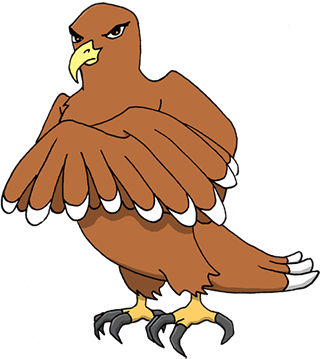
\includegraphics[width=4cm]{logo}}
\fi

%\renewcommand{\submittedtext}{change the default text here if needed}
\degree{Philosophi{\ae} Doctor (PhD)}
\degreedate{\todo{Add proper date}}


% ----------------------------------------------------------------------

% turn of those nasty overfull and underfull hboxes
\hbadness=10000
\hfuzz=50pt

% make blank pages really blank
\usepackage{emptypage}


%: --------------------------------------------------------------
%:                  FRONT MATTER: dedications, abstract,..
% --------------------------------------------------------------

\addbibresource{backmatter/references.bib}
\DeclareBibliographyCategory{onlyfullcite}
\newcommand\onlyfullcite[1]{\fullcite{#1}\addtocategory{onlyfullcite}{#1}}

\begin{document}

%\language{english}

% sets line spacing
\renewcommand\baselinestretch{1.2}
\baselineskip=18pt plus1pt


%: ----------------------- generate cover page ------------------------

\maketitle  % command to print the title page with above variables


%: ----------------------- cover page back side ------------------------
% Your research institution may require reviewer names, etc.
% This cover back side is required by Dresden Med Fac; uncomment if needed.

\newpage
\vspace{10mm}
\textbf{1$^{st}$ Advisor: Joaquim Gabarró Vallés}\\
\indent Universitat Politècnica de Catalunya, Barcelona, Spain

\vspace{10mm}
\textbf{2$^{nd}$ Advisor: Michael Hausenblas}\\
\indent Digital Enterprise Research Institute, Galway, Ireland\\
\indent MapR Technologies, San Jose, CA, USA

\vspace{20mm}
\textbf{Day of the defense:} \todo{add date of the defense}

\vspace{20mm}
\hspace{70mm}Signature from head of PhD committee:

%: ----------------------- abstract ------------------------

% Your institution may have specific regulations if you need an abstract and where it is to be placed in the document. The default here is just after title.

\begin{abstracts}

\textbf{(i) Mobile devices and social networks are omnipresent}

Mobile devices such as smartphones, tablets, or digital cameras
together with social networks enable people to create,
share, and consume enormous amounts of media items
like videos or photos both on the road or at home.
Such mobile devices---by pure definition---accompany
their owners almost wherever they may go.
In consequence, mobile devices are omnipresent
at all sorts of events to capture noteworthy moments.
Exemplary events can be keynote speeches at conferences,
music concerts in stadiums,
or even natural catastrophes like earthquakes
that affect whole areas or countries.
At such events---given a~stable network connection---part of
the event-related media items are published on social networks
both as the event happens or afterwards,
once a~stable network connection has been established again.

\textbf{(ii) Finding representative media items
for an event is hard}

Common media item search operations,
for example, searching for \emph{the} official video clip
for a~certain hit record on an online video platform
can in the simplest case be achieved based on potentially
shallow human-generated metadata
or based on more profound content analysis techniques
like optical character recognition,
automatic speech recognition,
or acoustic fingerprinting.
More advanced scenarios, however, like retrieving all
(or just the most representative) media items
that were created at a~given event
with the objective of creating \emph{event summaries} or
\emph{media item compilations} covering the event in question
are hard, if not impossible, to fulfill at large scale.
The main research question of this thesis
can be formulated as follows.

\textbf{(iii) Research question}

\textit{``Can user-customizable media galleries
that summarize given events be\linebreak
created solely based on textual and multimedia data
from social networks?''}

\textbf{(iv) Contributions}

In the context of this thesis, we have developed and evaluated
a~novel interactive application and related methods
for media item enrichment,
leveraging social networks, utilizing the Web of Data,
techniques known from Content-based Image Retrieval~(CBIR)
and Content-based Video Retrieval~(CBVR),
and fine-grained media item addressing schemes
like Media Fragments URIs
to provide a~scalable and near realtime solution
to realize the abovementioned scenario
of event summarization and media item compilation.

\textbf{(v) Methodology}

For any event with given event title(s),
(potentially vague) event location(s), and
(arbitrarily fine-grained) event date(s),
our approach can be divided in the following six steps.

\begin{enumerate}
  \item Via the textual search APIs (Application Programming Interfaces) of
        different social networks,
        we retrieve a~list of potentially event-relevant
        microposts that either contain media items directly,
        or that provide links to media items
        on external media item hosting platforms.
  \item Using third-party
        Natural Language Processing (NLP) tools,
        we recognize and disambiguate named entities
        in microposts to predetermine their relevance.
  \item We extract the binary media item data
        from social networks or media item hosting platforms
        and relate it to the originating microposts.
  \item Using CBIR and CBVR techniques, we first deduplicate
        exact-duplicate and near-duplicate media items
        and then cluster similar media items.
  \item We rank the deduplicated and clustered list
        of media items and their related microposts
        according to well-defined ranking criteria.
  \item In order to generate interactive and user-customizable
        media galleries that visually and audially summarize the
        event in question, we compile the top-$n$ ranked
        media items and microposts in aesthetically pleasing
        and functional ways.
\end{enumerate}
\end{abstracts}


% The original template provides and abstractseparate environment, if your institution requires them to be separate. I think it's easier to print the abstract from the complete thesis by restricting printing to the relevant page.
% \begin{abstractseparate}
%   \begin{abstracts}

\textbf{(i) Mobile devices and social networks are omnipresent}

Mobile devices such as smartphones, tablets, or digital cameras
together with social networks enable people to create,
share, and consume enormous amounts of media items
like videos or photos both on the road or at home.
Such mobile devices---by pure definition---accompany
their owners almost wherever they may go.
In consequence, mobile devices are omnipresent
at all sorts of events to capture noteworthy moments.
Exemplary events can be keynote speeches at conferences,
music concerts in stadiums,
or even natural catastrophes like earthquakes
that affect whole areas or countries.
At such events---given a~stable network connection---part of
the event-related media items are published on social networks
both as the event happens or afterwards,
once a~stable network connection has been established again.

\textbf{(ii) Finding representative media items
for an event is hard}

Common media item search operations,
for example, searching for \emph{the} official video clip
for a~certain hit record on an online video platform
can in the simplest case be achieved based on potentially
shallow human-generated metadata
or based on more profound content analysis techniques
like optical character recognition,
automatic speech recognition,
or acoustic fingerprinting.
More advanced scenarios, however, like retrieving all
(or just the most representative) media items
that were created at a~given event
with the objective of creating \emph{event summaries} or
\emph{media item compilations} covering the event in question
are hard, if not impossible, to fulfill at large scale.
The main research question of this thesis
can be formulated as follows.

\textbf{(iii) Research question}

\textit{``Can user-customizable media galleries
that summarize given events be\linebreak
created solely based on textual and multimedia data
from social networks?''}

\textbf{(iv) Contributions}

In the context of this thesis, we have developed and evaluated
a~novel interactive application and related methods
for media item enrichment,
leveraging social networks, utilizing the Web of Data,
techniques known from Content-based Image Retrieval~(CBIR)
and Content-based Video Retrieval~(CBVR),
and fine-grained media item addressing schemes
like Media Fragments URIs
to provide a~scalable and near realtime solution
to realize the abovementioned scenario
of event summarization and media item compilation.

\textbf{(v) Methodology}

For any event with given event title(s),
(potentially vague) event location(s), and
(arbitrarily fine-grained) event date(s),
our approach can be divided in the following six steps.

\begin{enumerate}
  \item Via the textual search APIs (Application Programming Interfaces) of
        different social networks,
        we retrieve a~list of potentially event-relevant
        microposts that either contain media items directly,
        or that provide links to media items
        on external media item hosting platforms.
  \item Using third-party
        Natural Language Processing (NLP) tools,
        we recognize and disambiguate named entities
        in microposts to predetermine their relevance.
  \item We extract the binary media item data
        from social networks or media item hosting platforms
        and relate it to the originating microposts.
  \item Using CBIR and CBVR techniques, we first deduplicate
        exact-duplicate and near-duplicate media items
        and then cluster similar media items.
  \item We rank the deduplicated and clustered list
        of media items and their related microposts
        according to well-defined ranking criteria.
  \item In order to generate interactive and user-customizable
        media galleries that visually and audially summarize the
        event in question, we compile the top-$n$ ranked
        media items and microposts in aesthetically pleasing
        and functional ways.
\end{enumerate}
\end{abstracts}

% \end{abstractseparate}


%: ----------------------- tie in front matter ------------------------

\frontmatter
\begin{dedication} %this creates the heading for the dedication page
To Laura, Lena, Emma, and Nil.
\end{dedication}

\begin{acknowledgements}

\textbf{Personal Acknowledgements:}

First and foremost, I~would like to thank my wife Laura
for her support, understanding, patience, and energy
during my time as a~PhD student, and simply for being at my side.
Without you, I~would not be where I~am today.

I~wholeheartedly thank my two advisors Joaquim Gabarró Vallés
and Michael Hausenblas for their guidance, helpful comments,
informative pointers, and especially
for their constructive criticisms.
The areas of research that I~have tackled in this thesis
are still young and sometimes uncharted territory.
I~am very thankful that the two of you have ventured
on the undertaking of leading me through this thesis.

I~deeply appreciate all the review comments, thoughts, challenging questions,
and, last not least, the \LaTeX~help of my dear friend
and research colleague Ruben Verborgh.
It was, is, and will be an honor to work with you.
My warm thanks also go to Raphaël Troncy and his team
at \mbox{EURECOM} Sophia Antipolis in France
who have helped shape some of the ideas presented in this thesis.

I~would like to thank my former and current managers at Google,
namely N.~Kryvossidis, R.~Ashley, C.~Bouchère, and I.~Sassarini
for their support for my thesis.
A~lot of valuable input for my thesis came in via social networks.
My thanks go out to everyone I have interacted with
around the hashtag \texttt{\#TomsPhD}
on Twitter, \googleplus, and Facebook.

Finally, I~sincerely thank my parents and my brother
who have made me the person I~am today.
My parents have taught me
not to go for the easy choices, even
if at times they may seem tempting,
but instead to try harder and never give up.
This thesis also is for you.

\textbf{Formal Acknowledgements:}

The research presented in this thesis
was partially supported by the European Commission
under Grant No. 248296 with the European Union (FP7 ICT STReP)
project \mbox{\emph{I-SEARCH}}.

\vspace{80mm}

\textbf{To cite this document:}

\small
\begin{verbatim}
  @phdthesis{steiner2013thesis,
    author = {Thomas Steiner},
    title  = {Enriching Unstructured Media Content About Events to
              Enable Semi-Automated Summaries, Compilations, and
              Improved Search by Leveraging Social Networks},
    year   = {2013},
    school = {Universitat Polit\`{e}cnica de Catalunya}
  }
\end{verbatim}

\normalsize

\vspace{10mm}
\textbf{Copyright and License:}\\\\
\small \copyright \normalsize 2013 Thomas Steiner\\
Licensed under the Creative Commons Attribution-ShareAlike 3.0 License.\\
\url{http://creativecommons.org/licenses/by-sa/3.0/}

\end{acknowledgements}



%: ----------------------- contents ------------------------

\setcounter{secnumdepth}{2} % organisational level that receives a numbers

% make sure that subsubsections without numbering are still indented correctly
\makeatletter
\renewcommand{\l@subsubsection}{\@dottedtocline{3}{9em}{2.3em}}
\makeatother

\setcounter{tocdepth}{3}    % print table of contents for level 3
\tableofcontents            % print the table of contents

% levels are: 0 - chapter, 1 - section, 2 - subsection, 3 - subsection


%: ----------------------- list of figures/tables ------------------------

\listoffigures  % print list of figures

\addcontentsline{toc}{chapter}{List of Listings}
\lstlistoflistings % print list of listings

\listoftables  % print list of tables

%: ----------------------- glossary ------------------------

% Tie in external source file for definitions: /frontmatter/glossary.tex
% Glossary entries can also be defined in the main text. See glossary.tex
% this file is called up by thesis.tex
% content in this file will be fed into the main document

% Glossary entries are defined with the command \nomenclature{1}{2}
% 1 = Entry name, e.g. abbreviation; 2 = Explanation
% You can place all explanations in this separate file or declare them in the middle of the text. Either way they will be collected in the glossary.

% required to print nomenclature name to page header
\markboth{\MakeUppercase{\nomname}}{\MakeUppercase{\nomname}}

\nomenclature{NLP}{Natural Language Processing}
\nomenclature{CBIR}{Content-based Image Retrieval} 
\nomenclature{CBVR}{Content-based Video Retrieval} 
\nomenclature{RDF}{Resource Description Framework}
\nomenclature{W3}{World-Wide Web}
\nomenclature{WWW}{World-Wide Web}
\nomenclature{CERN}{European Organization for Nuclear Research}
\nomenclature{HTML}{Hypertext Markup Language}
\nomenclature{URI}{Unique Resource Identifier}
\nomenclature{URL}{Unique Resource Locator}
\nomenclature{JSON}{JavaScript Object Notation}
\nomenclature{Turtle}{Terse RDF Triple Language}
\nomenclature{CURIE}{Compact URI}
\nomenclature{SPARQL}{SPARQL Protocol and RDF Query Language}
\nomenclature{W3C}{World Wide Web Consortium}
\nomenclature{LOD}{Linking Open Data}
\nomenclature{SNS}{Social Network(ing) Site}
\nomenclature{API}{Application Programming Interface}
\nomenclature{NEE}{Named Entity Extraction}
\nomenclature{NER}{Named Entity Recognition}
\nomenclature{OWL}{Web Ontology Language}
\nomenclature{DOM}{Document Object Model}
\nomenclature{POS}{Part-of-Speech (tagging)}

\begin{multicols}{2} % \begin{multicols}{#columns}[header text][space]
\begin{footnotesize} % scriptsize(7) < footnotesize(8) < small (9) < normal (10)

\printnomenclature[1.5cm] % [] = distance between entry and description
\label{nom} % target name for links to glossary

\end{footnotesize}
\end{multicols}



%: --------------------------------------------------------------
%:                  MAIN DOCUMENT SECTION
% --------------------------------------------------------------

% the main text starts here with the introduction, 1st chapter,...
\mainmatter

\renewcommand{\chaptername}{} % uncomment to print only "1" not "Chapter 1"
\renewcommand\chapterautorefname{Chapter}

%: ----------------------- subdocuments ------------------------

% Parts of the thesis are included below. Rename the files as required.
% But take care that the paths match. You can also change the order of appearance by moving the include commands.

\chapter{Event Summarization Challenge}
\label{cha:introduction}

% the code below specifies where the figures are stored
\ifpdf
    \graphicspath{{1_introduction/figures/PNG/}{1_introduction/figures/PDF/}{1_introduction/figures/}}
\else
    \graphicspath{{1_introduction/figures/EPS/}{1_introduction/figures/}}
\fi

\section{Motivation and Problem Statement}

A~very open definition of the word \emph{event}
given by WordNet~\cite{fellbaum1998wordnet,miller1995wordnet} is
\emph{``something that happens at a~given place and time''}.
Following this definition,
we are indeed surrounded by events,
most of which are of little to no interest for us.
A~concert somewhere in the world of a~band
that we do not even know may be a~good example.
For some events, however, we may care more, for example,
a~concert of a~band that we know and like,
even if it takes place at a~location far away from us.
Finally, for very few events, we may care a~lot,
maybe even enough to physically attend the event,
like a~concert of our favorite band
if it takes place in our city, is not sold out,
and not too expensive.

All this motivates the need for \emph{event summarization}.
If there is an event that we could not attend
for any given reason,
but that we are interested in,
a~good event summarization can help us get a~feeling
for the event's atmosphere.
Similarly, if there is an event that we attended,
we can revive the event's most fascinating moments
based on the event summarization.

A~\emph{media gallery} in the context of
our event summarization task is
a~\emph{best-of} compilation of photos, videos,
and microposts retrieved from social networks
that are related to a~given event.
Event summarization covers textual
as well as multimedia content.
We say a~media gallery is of high quality,
if it fulfills the following properties.

\begin{enumerate}
  \item \textit{Conciseness:}
        it conveys a~lot of information clearly
        and in few media items.
  \item \textit{Comprehensiveness:}
        it is complete and covers all representative
        elements or aspects of an event.
  \item \textit{Authenticity:}
        it is of undisputed origin and genuine.
  \item \textit{Diversity:}
        it shows a~great deal of variety.
  \item \textit{Interestingness:}
        it catches and holds the attention of the viewer.     
\end{enumerate}

\section{Research Question and Hypothesis}

The main research question for this thesis
can be formulated as follows.
 
\textit{``Can user-customizable
media galleries that summarize given events be
created solely based on textual and multimedia data
from social networks?''}

\noindent The hypothesis that we test in this thesis
can be formulated as follows.

We argue that through media galleries that leverage content
that was shared on social networks,
a~more \emph{authentic}, more \emph{concise},
more \emph{comprehensive}, more \emph{diverse},
and also more \emph{interesting}
view on events gets possible than by limiting oneself
to officially produced media content;
and that further such media galleries can be generated
more \emph{efficiently} and \emph{in shorter time}
than manually produced media galleries.

We validate these subjective and objective
criteria with experiments for events of different categories
such as sports, politics, culture, leisure,
music, conferences, \emph{etc.}

\section{Approach}

The objective of this thesis is the development
of methods for the automated summarization of events
based on media items shared on social networks.
A~schematic overview of the approach can be seen
in~\autoref{fig:thesis-diagram}.
As an event takes places and shortly thereafter
(symbolized by the timeline marked with \emph{2h Event}),
people share media items related to the event
on multiple social networks
(symbolized by the photo and video pictograms
above the event timeline).
Via the textual search APIs (Application Programming Interfaces)
of these different social networks,
we retrieve a~list of potentially event-relevant
microposts that either contain media items directly,
or that provide links to media items
on external media item hosting platforms.
Using third-party NLP tools,
we recognize and disambiguate named entities
in the microposts to predetermine their relevance.
We extract the binary media item data
from social networks or media item hosting platforms
and relate it to the originating microposts
(symbolized by the central cloud).
Using CBIR and CBVR techniques, we first deduplicate
duplicate and near-duplicate media items,
and then cluster similar media items
(symbolized by the green, red, and orange markers).
We rank the deduplicated and clustered list
of media items and their related microposts
according to well-defined ranking criteria.
In order to generate interactive and user-customizable
media galleries that visually and audially summarize the
event in question, we compile the top-$n$ ranked
media items and microposts in an aesthetic way
(symbolized by the timeline marked with \emph{5min Summary}).

\begin{figure}[!ht]
  \centering
  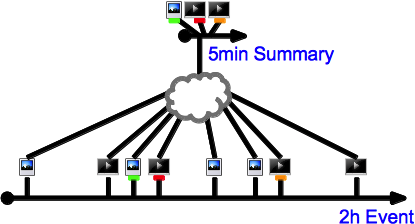
\includegraphics[]{thesis-diagram.png}
  \caption[Schematic depiction of event summary generation]
    {Schematic depiction of event summary generation
    based on deduplicated, clustered, and ranked media items
    for an exemplary event}
  \label{fig:thesis-diagram}
\end{figure}

\section{Contributions}

In this thesis, we report on methods for
the automated generation of event summaries.
This particular field of research touches on many related areas
of research and research communities,
amongst which social network research, multimedia content analysis,
Semantic Web and Natural Language Processing (NLP),
human factors in computing systems,
and Web services.
Early on in the process of this thesis,
we have sought and incorporated expert feedback based on
a~Doctoral Consortium paper~%
\cite{steiner2011enrichingunstructured}.
We have broken our contributions down into
the following topics.

\subsection{Social Network Multimedia and Data Analysis}

We have worked on methods for the aggregation, extraction,
deduplication, clustering, and compilation
of social media contents from
multiple social networks~%
\cite{rizzo2012whatfresh}.
Those methods were applied and evaluated
for the enhancement of conference experiences~%
\cite{khrouf2012aggregatingsocialmedia,khrouf2012confomaton}.

\subsection{Application of Semantic Web and NLP Techniques}

In order to make sense out of social network microposts,
we have worked on methods to consolidate and rank
the results of multiple named entity recognition and
disambiguation APIs and to track their data provenance~%
\cite{steiner2011addingmeaning}.
We have applied and evaluated those methods
for the consumer-oriented detection of trending microposts
on a~major commercial social network~%
\cite{steiner2011tweetconsumers}.


\subsection{Video Content and Metadata Analysis}

We have worked on methods for named entity extraction and
disambiguation for online videos based on closed captions
and other textual metadata, which make online video
more accessible, searchable, and interconnected~%
\cite{steiner2010semwebvid,steiner2010semwebvidchallenge}.
Further, we have combined those textual methods with 
video content analysis methods for the on-the-fly detection
of shot boundaries for online videos~%
\cite{steiner2012shotdetection}.
We have defined aesthetic principles
for the automated generation of media gallery layouts
for visual and audial event summarization
based on social network multimedia data~%
\cite{steiner2012definingaesthetic}.
        
\subsection{Crowdsourcing}

The video content analysis methods mentioned before
were combined with methods for the crowdsourced detection
of events in online videos~%
\cite{steiner2011crowdsourcingevent}.
We have further worked on crowdsourcing methods
for the extraction of knowledge items from arbitrary Web pages~%
\cite{steiner2012sekiathome,steiner2012sekiathomechallenge}.

\subsection{Studies}

We have contributed an examination of Linked Data usage and
visualization techniques of a~major commercial search engine~%
\cite{steiner2010howgoogleisusing}.
In addition to that, we have studied the usefulness and relevance
of social network updates which were added to search engine
results pages (SERP) of a~major commercial search engine~%
\cite{steiner2012addingrealtime}.

\subsection{Multimodal Search Engines}

We have worked on an examination of context-aware querying
for multimodal search engines~%
\cite{etzold2012contextawarequerying,steiner2012isearch}.
Further, we have studied user interface constraints on
mobile and desktop devices for a~multimodal search engine
and demonstrated that those constraints can be overcome~%
\cite{steiner2012onesizedoesnotfitall}.


\subsection{Web Service Description}

We have worked on methods for the semantic description of Web APIs,
their discoverability, their automated consumption,
their semantic interlinking, and their social aspects~%
\cite{verborgh2011descriptionandinteraction,verborgh2011efficientruntime,verborgh2011integratingdata,verborgh2012capturingthefunctionality,verborgh2012functionalcomposition,verborgh2012functionaldescriptions,verborgh2012missinglinks,verborgh2012restdesc,verborgh2012socialdescriptionrevolution}.
We have studied the feasibility of truly RESTful behavior
for Web APIs in the sense of Dr. Roy Fielding~%
\cite{steiner2011fulfilling}.
        
\subsection{Standardization and Specifications}        
We have helped to shape a~W3C specification on media
fragment addressing schemes for audio and video items~%
\cite{troncy2012mediafragments}.
Further, we have worked on the definition of a~unified framework
for the description of multimedia content objects~%
\cite{axenopoulos2012isearch,daras2011unifiedframework}.
Finally, we have contributed to a~white paper on the
Future Media Internet Architecture~%
\cite{alduan2011futureinternet}.

\subsection{Others}

We have developed methods for unobtrusively fixing
common annoyances on arbitrary Web pages~%
\cite{steiner2012xkcd37}.

\section{Thesis Structure}

The remainder of this thesis is structured as follows. 

\autoref{cha:background} introduces the Semantic Web and its technologies.
Starting from the non-semantic Web,
we show how structured data can be added to Web pages
and briefly present DBpedia as a~knowledge base
founded on structured data extracted from Wikipedia.
We then continue with the Resource Description Framework
and explain how it represents facts with triples.
We provide examples of RDF's different serialization formats.
Afterwards, we outline the Semantic Web vision of
a~global giant database and present the Semantic Web
query language SPARQL.
We close the chapter with an introduction of Sir Tim Berners-Lee's
Linked Data principles and show how data publisher that publish
datasets according to those principles are visualized in the
Linking Open Data cloud.

\autoref{cha:social-networks}
\autoref{cha:micropost-annotation}
\autoref{cha:eventdetection}
\autoref{cha:media-item-extraction}
\autoref{cha:shot-boundary-detection}
\autoref{cha:media-item-deduplication}
\autoref{cha:media-item-ranking}
\autoref{cha:media-item-compilation}
\autoref{cha:future-work}

Each chapter is closed by a~final section called
\emph{Chapter Notes}, which contains references to publications
that the chapter is based upon,
and in some cases pointers to related material for further reading.

\bibliographystyle{plainnat}
\clearpage
\bibliography{backmatter/references}

\chapter{Semantic Web Technologies}
\label{cha:background}

% the code below specifies where the figures are stored
\ifpdf
    \graphicspath{{2_background/figures/PNG/}{2_background/figures/PDF/}{2_background/figures/}}
\else
    \graphicspath{{2_background/figures/EPS/}{2_background/figures/}}
\fi

The main contributions of this thesis
are methods for the automated generation of
user-customizable media galleries
for the visual and audial summarization of events.
To provide context for the proposed approaches
in the later parts of the thesis,
we start with two introductory chapters
related to Semantic Web technologies
and social networks.
The current \autoref{cha:background} covers
the Semantic Web, Linked Data,
and the Resource Description Framework (RDF).
The following \autoref{cha:social-networks}
will cover social networks
by first providing a~definition
and classification of social networks,
and then introducing popular social networks
and some of their core features.

\section{The World Wide Web and Semantics}

Tim Berners Lee, inventor of the World Wide Web (W3, WWW),
or simply, the \emph{Web},
writes in~\cite{bernerslee1994worldwideweb}:
\textit{``The World Wide Web was developed
to be a~pool of human knowledge,
which would allow collaborators
in remote sites to share their ideas
and all aspects of a~common project''}.
Since its earliest days at CERN,
the European Organization for Nuclear Research
in Geneva, Switzerland,
the Web has scaled to a~truly global system
of interlinked hypertext documents
accessed via the Internet.

\emph{Semantics} is the study of meaning.
It focuses on the relation between
words, phrases, signs, and symbols,
and what they stand for, \emph{i.e.},
the actual object referred to by a~linguistic expression.
Michel Bréal can be counted as the founder
of modern semantics with his 1897
\emph{Essai de sémantique}~\cite{breal1897essai}.
The \emph{Semantic Web} brings these two worlds---the
World Wide Web and semantics---together.

\section{The Semantic Web}

The lexical database
WordNet~\cite{fellbaum1998wordnet,miller1995wordnet}
by the Cognitive Science Laboratory
of Princeton University defines the term \emph{semantic}
as \emph{``of or relating to meaning or the study of meaning''}.
The same source defines the term \emph{Web},
which is a~common form for the complete term
\emph{World Wide Web} as
\emph{``computer network consisting of a~collection of internet sites that offer text and graphics and
sound and animation resources through the hypertext
transfer protocol''}.
Finally, WordNet defines the term \emph{meaning}
as \emph{``the message that is intended or expressed
or signified''}, or \emph{``the idea that is intended''}.

The combined term \emph{Semantic Web} was coined
by Sir Tim Berners-Lee,
in a~May 2001 article co-published with James Hendler
and Ora Lassila
in the Scientific American~\cite{bernerslee2001semanticweb}.
Therein, the authors write: 

\begin{quotation}
\textit{``The Semantic Web will bring structure to the meaningful
content of Web pages,
creating an environment where software agents
roaming from page to page
can readily carry out sophisticated tasks for users. [\ldots]
The Semantic Web is not a~separate Web
but an extension of the current one,
in which information is given well-defined meaning,
better enabling computers and people
to work in cooperation.
The first steps in weaving the Semantic Web
into the structure of the existing Web
are already under way.
In the near future, these developments
will usher in significant new functionality
as machines become much better able to process and \emph{understand} the data
that they merely display at present.''}
\end{quotation}

We are currently experiencing a~fundamental shift
from the World Wide Web to the Semantic Web,
a~shift from moving bits to moving bits with a~meaning.
This can have a~huge impact,
which might not be as drastic as Tim Berners-Lee describes
in his Scientific American article,
but which might introduce many improvements,
like more accurate search results,
more intelligent price comparison services, \emph{etc.}
\autoref{fig:fundamental-shift} illustrates this idea.

\begin{figure}[!ht]
\centering
  \subfloat[Bits without meaning.]{
    \label{fig:fundamental-shift-1}
    
\includegraphics[width=0.3\textwidth]{fundamental-shift-1.png}
   }                
  \subfloat[Bits with a~meaning.]{
    \label{fig:fundamental-shift-2}
    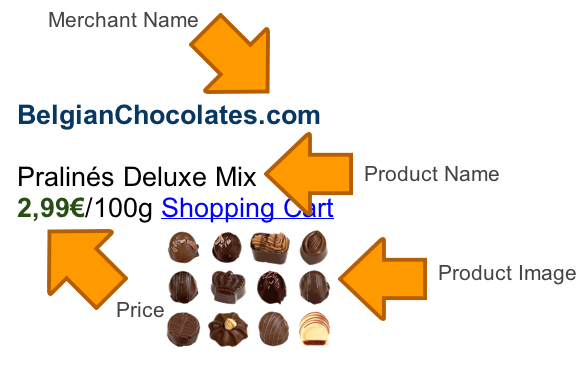
\includegraphics[width=0.468\textwidth]{fundamental-shift-2.png}
  }
  \caption{Fundamental shift from moving bits to moving bits with a~meaning}
  \label{fig:fundamental-shift}  
\end{figure}

\subsection{The Non-Semantic Web} \label{sec:non-semantic-web}

To differentiate the Semantic Web from the non-semantic Web,
it helps to step back one step and
see why the non-semantic Web is not semantic.
The Web is a~system of interlinked hypertext documents
accessed through the Internet.
These documents are typically marked up in
the Hypertext Markup Language (HTML),
a~language that defines a~syntax
understandable to user agents like Web browsers,
however, not one that provides meaning
beyond the level of text layout.
This means that an HTML snippet like
\begin{verbatim}
<h1>The Catcher in the Rye</h1>
<h2>J. D. Salinger</h2>
\end{verbatim}
reveals that \emph{The Catcher in the Rye}
is a~level one header element and
that \emph{J. D. Salinger} a~level two header element,
but to a~machine it is not evident that the prior
is the title of a~book,
and that the latter is (i) an author, and (ii)
the author of \emph{The Catcher in the Rye}.

\subsection{Structured Data on the Web}

A~very first step towards adding semantics to the Web
is using tabular data.
\autoref{tab:sample-table-structured-data} shows an example
for such tabular data.
For human beings (interested in sports),
the meaning of the columns in
\autoref{tab:sample-table-structured-data} is clear:

\begin{small_itemize}
  \item[] P = matches \textbf{P}layed
  \item[] W = \textbf{W}ins 
  \item[] D = \textbf{D}raws
  \item[] L = \textbf{L}osses
  \item[] F = Goals \textbf{F}or
  \item[] A = Goals \textbf{A}gainst
  \item[] Pts = \textbf{P}oin\textbf{ts}
\end{small_itemize}

\begin{table}[!ht]
\centering
    \begin{tabular}{l*{6}{c}r}
Team              & P & W & D & L & F  & A & Pts \\
\hline
Manchester United & 6 & 4 & 0 & 2 & 10 & 5 & 12  \\
Celtic            & 6 & 3 & 0 & 3 &  8 & 9 &  9  \\
Benfica           & 6 & 2 & 1 & 3 &  7 & 8 &  7  \\
FC Copenhagen     & 6 & 2 & 1 & 2 &  5 & 8 &  7  \\
    \end{tabular}
    \caption{Sample table with structured data for sports results}
    \label{tab:sample-table-structured-data}
\end{table}

The problem, however, is for machines to understand
the structure of the table.
Let us imagine one wanted to automate the task
of retrieving sports results from a~Web page with tabular data.
While it is a~straightforward job to implement
a~scraper bot that searches for column titles
like ``P'', ``W'', ``D'', \emph{etc.},
it would require the same work over and over again
for a~different language,
for example, German, where the terms would be:
``Sp.''~(Spiele), ``g.''~(gewonnen), ``u.''~(unentschieden),
``v.''~(verloren), ``Tore''~(Tore), ``Pkte.''~(Punkte).
A~German-speaking reader might have noticed
that the exemplary German system listed here
does not differentiate between \emph{goals for}
and \emph{goals against}, but only has a~list of \emph{Goals}.
Tiny differences like this make the scraping approach brittle.
If data providers were to use unique column identifiers like
Unique Resource Identifiers (URIs),
the problem would be easier.
In the concrete example for English and German,
rather than using ``D'' (\emph{Draws})
and ``u.'' (\emph{unentschieden}),
which both mean that the result was a~tie,
the machine-readable column name could instead be identified by
a~\emph{Unique} Resource Identifier (URI) like
\url{http://dbpedia.org/page/Tie_(draw)},
or even a~fictive URI like \url{http://example.org/VGllXyhkcmF3KQ==}.
In the next section, we therefore introduce
the structured knowledge base and interlinking hub
in the Web of Data, DBpedia~\cite{auer2007dbpedia}.

\subsection{The Structured Knowledge Base DBpedia}

An often reoccurring pattern
in the Semantic Web world
is the use of DBpedia~\cite{auer2007dbpedia}
as a~hub for identifying concepts by URIs.
DBpedia is a~Semantic Web knowledge base
with the objective of automatically extracting
pre-structured tabular data from the human-generated info-boxes
from the online encyclopedia
Wikipedia.\footnote{\url{http://en.wikipedia.org/wiki/Main_Page},
accessed July 15, 2013}
This pre-structured information is then made available
on the World Wide Web in many formats,
for example, in JSON~\cite{crockford2006json}
and many RDF~\cite{klyne2004rdf} serializations.
DBpedia allows for querying relationships
and properties associated with Wikipedia resources,
including links to other related datasets.
As outlined before, the concept of a~tie draw
in the sense of sports could thus be uniquely identified
by the DBpedia URI \url{http://dbpedia.org/page/Tie_(draw)},
free of all ambiguity.
Similar knowledge bases are among others
Freebase~\cite{markoff2007freebase},
YAGO~\cite{suchanek2007yago}, and CYC~\cite{lenat1995cyc}.

\subsection{Semantics in HTML Versions 4.01 and 5}

As outlined in \autoref{sec:non-semantic-web},
HTML versions 4.01~\cite{raggett1999html}
and 5~\cite{berjon2012html5}
contain a~basic level of semantics.
The main focus, however, is on the separation of
the markup of the textual structure from the actual presentation.
For example the \texttt{<b>} and the \texttt{<strong>} tags
both have the same visual effect:
they make the node value appear in a~bold face \textbf{like so}.
Visually, there is no way to differentiate between the two,
however, semantically the difference exists and is well-defined:
\texttt{<strong>} should be used when
one wants to give special emphasis on something.
Screen readers will typically read out such text
with a~more emphasized voice.
In contrast, \texttt{<b>} should be used
if only visually one wants to create a~bold face look.
In the following, we present a~list of semantic HTML tags
and attributes and their meaning.

\paragraph{Semantic HTML 4.01 Tags:}

\begin{itemize}
  \item \texttt{<abbr>} specifies an abbreviation,
        \texttt{<acronym>} specifies an acronym.
  \item \texttt{<h1>--<h6>} specify level 1--6 headers,
        \texttt{<caption>} specifies a~caption for a~table.
  \item \texttt{<blockquote>} specifies a~block-level quotation
        (a~source in form of a~URI may be specified via the
        \texttt{cite} attribute),
        \texttt{<cite>} specifies a~citation.
  \item \texttt{<dl>} specifies a~definition list, \texttt{<dt>}
        specifies a~definition term in a~definition list,
        \texttt{<dd>} specifies the definition of a~term
        in a~definition list.
  \item \texttt{<em>} specifies an emphasis, \texttt{<strong>}
        specifies a~strong emphasis.
  \item \texttt{<code>} specifies a~code snippet, \texttt{<dfn>}
        specifies an inline definition of a~single term,
        \texttt{<address>} specifies contact information
        for the document author, \texttt{<legend>} specifies
        a~legend for \texttt{<fieldset>} containers
        for adding structure to forms,
        \texttt{<samp>} specifies sample output
        from a~script or program.
\end{itemize}

\paragraph{Semantic HTML5 Tags:}

\begin{itemize}
  \item \texttt{<article>} specifies an independent item
        section of content,
        \texttt{<aside>} specifies a~section of a~page that
        consists of content that is tangentially related
        to the content around the \texttt{<aside>} element,
        and which could be considered separate from
        that content, \texttt{<header>} specifies a~group of
        introductory or navigational aids,
        \texttt{<footer>} specifies a~footer for its nearest
        ancestor sectioning content or sectioning root element,
        \texttt{<nav>} specifies a~section with navigation links.
  \item \texttt{<figure>} specifies some flow content,
        \texttt{<mark>} specifies a~run of text in one document
        marked or highlighted for reference purposes
        due to its relevance in another context,
        \texttt{<meter>} specifies a~scalar measurement within
        a~known range, or a~fractional value.
  \item \texttt{<audio>} specifies a~sound or an audio stream,
        \texttt{<video>} specifies a~video or movie.
  \item \texttt{<progress>} specifies the completion progress
        of a~task, \texttt{<time>} specifies either a~time
        on a~24 hour clock, or a~precise date in the calendar
        (optionally with a~time and a~time-zone offset),
        \texttt{<command>} specifies a~command that the user
        can invoke.
  \item \texttt{<details>} specifies a~disclosure widget
        from which the user can obtain additional information or
        controls, \texttt{<datalist>} specifies the list that
        represents predefined options for input elements.
  \item \texttt{<keygen>} specifies a~key pair generator control,
        \texttt{<output>} specifies the result of a~calculation,
        \texttt{<ruby>} allows one or more spans of phrasing
        content to be marked with ruby annotations.
\end{itemize}

\paragraph{HTML5 Input Type Attributes:}

\begin{itemize}
  \item \texttt{datetime} specifies a~control for setting the
        element’s value to a~string representing a~global date
        and time (with timezone information).
  \item \texttt{datetime-local} specifies a~control for setting
        the element’s value to a~string representing a~local date
        and time (with no timezone information).
  \item \texttt{date} specifies a~control for setting the 
        element’s value to a~string representing a~date,
        \texttt{month} specifies a~control for setting the
        element’s value to a~string representing a~month,
        \texttt{week} specifies a~control for setting the
        element’s value to a~string representing a~week.
  \item \texttt{time} specifies a~control for setting the
        element’s value to a~string representing a~time
        (with no timezone information).
  \item \texttt{number} specifies a~control for setting the
        element’s value to a~string representing a~number.
  \item \texttt{range} represents an imprecise control
        for setting the element’s value to a~string
        representing a~number.
  \item \texttt{email} specifies a~control for editing
        a~list of email addresses given in the element’s value.
  \item \texttt{url} specifies a~control for editing an
        absolute URL given in the element’s value.
  \item \texttt{search} specifies a~one-line plain-text
        edit control for entering one or more search terms.
  \item \texttt{color} specifies a~color-well control for
        setting the element’s value to a~string representing
        a~simple color.
\end{itemize}

\subsection{Structured Data Beyond Pure HTML}

In this subsection, we describe how structured data
can be included in HTML documents
by either overloading existing HTML attributes
or by adding new ones.

\subsubsection{Microformats}

Microformats~\cite{celik2006microformats} are a~set of
open data mark-up formats developed
and defined by the Microformats
community.\footnote{\url{http://microformats.org/discuss},
accessed July 15, 2013}
Microformats are not an official standard,
but rather a~widely adopted grass-roots-driven movement
with origins in the blogging scene.
It is to be noted that Microformats do not require a~new language,
but reuse building blocks from widely adopted standards
such as the \texttt{class}, \texttt{rel}, and \texttt{title}
attributes in HTML.
Their main design goal is to focus first on humans,
then on machines.
A~concrete example of Microformat mark-up in HTML
can be seen in \autoref{code:microformats}.
There are currently nine stable
Microformats,\footnote{\url{http://microformats.org/wiki/Main_Page\#Specifications}, accessed July 15, 2013}
as listed below:

\begin{itemize}
  \item \texttt{hCalendar} is a~distributed calendaring and
        events format, using a~1:1 representation of the standard
        \texttt{iCalendar} format
        (RFC~2445,~\cite{dawson1998icalendar}).
  \item \texttt{hCard} is a~format for representing people,
        companies, organizations, and places, using a~1:1
        representation of the standard \texttt{vCard} format
        (RFC~2426,~\cite{dawson1998vcard}).
  \item \texttt{rel-license} is a~format for indicating content
        licenses, which is embeddable in
        HTML~\cite{raggett1999html} or
        XHTML~\cite{pemberton2000xhtml},
        Atom~\cite{nottingham2005atom},
        RSS~\cite{cadenhead2006rss},
        and arbitrary XML~\cite{bray2008xml}.
  \item \texttt{rel-nofollow} is a~format for hyperlinks
        indicating that the destination of that hyperlink should
        not be afforded any additional weight or ranking by user
        agents such as search engines, which perform link
        analysis upon Web pages.
  \item \texttt{rel-tag} is a~format for hyperlinks indicating
        that the destination of that hyperlink is an
        author-designated keyword for the current page.
  \item \texttt{VoteLinks} is a~format for adding the idea of
        agreement, abstention or indifference, and disagreement
        to hyperlinks.
  \item \texttt{XFN} is a~format for representing human
        relationships using hyperlinks, which enables Web authors
        to indicate their relationships to people.
  \item \texttt{XMDP} is a~format for defining metadata profile
        documents (XHTML Meta Data Profile), which enables Web
        authors to well-define custom meta tags.
  \item \texttt{XOXO} is a~format for defining a~new
        XHTML~\cite{pemberton2000xhtml}
        document type for subsetting and extending XHTML,
        which serves as the basis for XHTML-friendly outlines for
        processing by XML engines, and for easy interactive
        rendering by browsers.
\end{itemize}

\begin{lstlisting}[caption={
   [Sample code snippet with embedded hCard Microformat mark-up]
   {Sample code snippet with embedded \texttt{hCard} Microformat
    mark-up (\url{http://microformats.org/wiki/hcard})}
  },
  label={code:microformats}]
<div class="vcard">
  <a class="fn org url" href="http://www.commerce.net/">CommerceNet</a>
  <div class="adr">
    <span class="type">Work</span>:
    <div class="street-address">169 University Avenue</div>
    <span class="locality">Palo Alto</span>,  
    <abbr class="region" title="California">CA</abbr>&nbsp;&nbsp;
    <span class="postal-code">94301</span>
    <div class="country-name">USA</div>
  </div>
  <div class="tel">
   <span class="type">Work</span> +1-650-289-4040
  </div>
  <div class="tel">
    <span class="type">Fax</span> +1-650-289-4041
  </div>
  <div>Email: 
   <span class="email">info@commerce.net</span>
  </div>
</div>
\end{lstlisting}

\subsubsection{Microdata}

Microdata~\cite{hickson2012microdata} defines a~way to annotate 
content (or items) with specific machine-readable labels,
for example, to allow scripts to provide services that are
customized to a~website.
Microdata allows for nested groups of name-value pairs
to be added to documents,
in parallel with the existing content.
The Microdata specification introduces
a~set of new attributes to HTML:

\begin{itemize}
  \item \texttt{itemscope} creates an item (or thing) and
        indicates that descendants of this element contain
        information about it. This attribute precedes the
        \texttt{itemtype} attribute in the HTML element's tag.
  \item \texttt{itemtype} a~valid URL of a~vocabulary that
        describes the item and its properties context.
  \item \texttt{itemid} indicates a~unique identifier
        of the item in the vocabulary.
  \item \texttt{itemprop} indicates that its containing tag
        holds the value of the specified item property.
        The properties name and value context are described by
        the items vocabulary. Properties values usually
        consist of string values,
        but can also use URLs using the \texttt{<a>} tag
        and its \texttt{href} attribute,
        the \texttt{<img>} tag and its \texttt{src} attribute,
        or other tags that link to or embed external resources.
  \item \texttt{itemref} properties that are not descendants of
        the element with the \texttt{itemscope} attribute
        can be associated with the item using this attribute.
        It provides a~list of elements to Web crawlers to find
        additional property values of the item
        elsewhere in the document.
\end{itemize}

An example of Microdata in HTML can be seen in \autoref{code:microdata}.

\begin{lstlisting}[caption={
  [Sample code snippet with Microdata mark-up]
  {Sample code snippet with Microdata mark-up
   (\url{http://www.w3.org/TR/microdata/})}},
  label={code:microdata}]
<div itemscope>
  <p>My name is <span itemprop="name">Neil</span>.</p>
  <p>
    My band is called
    <span itemprop="band">Four Parts Water</span>.
  </p>
  <p>I am <span itemprop="nationality">British</span>.</p>
</div>
\end{lstlisting}

\section{Resource Description Framework (RDF)} \label{sec:rdf}

The Resource Description Framework (RDF,~\cite{klyne2004rdf})
defines a~set of W3C standards for the formal description of
resources that are identified by URIs.
RDF is a~core component of the Semantic Web.
Initially, it was designed to describe metadata
on the World Wide Web (WWW) such as authors,
copyrights, \emph{etc.}\ of documents, however,
applying a~definition of the term \emph{resource}
beyond the WWW context,
RDF is now also used to describe metadata
of any URI-identifiable entity like cities, genes, \emph{etc.}

\subsection{Triples as a~Data Structure}

As outlined before, one of the main purposes of the Semantic Web
is to give information a~well-defined meaning.
Using an example from Tim Berners-Lee’s
article~\cite{bernerslee2001semanticweb},
meaning can be to differentiate between the concepts of
a~shipping and a~billing address,
or the concept of an address in the sense of
delivering a~formal spoken communication to an audience.
In order to assure the differences in meaning,
things are identified by a~Unique Resource Identifier (URI).
The majority of the data processed by machines
can be described by elementary sentences like
\emph{A~cat is a~mammal},
\emph{Thomas Steiner is the author of this document},
or \emph{Prince William is married to Kate Middleton}.
Each of these sentences has a~subject (\emph{A~cat}),
a~predicate (\emph{is a}), and an object (\emph{mammal}).
Every subject, predicate, and object can be identified by a~URI.
This idea is very powerful,
as it allows to express the same concept
represented by a~URI (for example, mammal by
\url{http://dbpedia.org/resource/Mammal})
with different terms in different languages
(like, for example, Säugetier, mammal, or nisäkkäät).
Everyone can extend the set of concepts
simply by creating a~URI on the Web.
This form of knowledge representation
is used by the Resource Description Framework.

\subsection{Important RDF Serialization Syntaxes}

Knowledge or facts represented in the RDF triple data structure
need to be serialized in order to be stored
or transmitted over the Internet.
Several serialization formats exist,
each of which with its particular advantages
and disadvantages, mostly around readability for human beings
and parsability for machines.
According to our experience, most people prefer the Turtle~\cite{prudhommeaux2013turtle}
format for its readability,
whereas for machines, oftentimes RDF/XML~\cite{beckett2004rdfxml}
is the easiest to work with.

\subsubsection{RDF Sample Graph}
In the following, we will illustrate the various
RDF serialization formats with an RDF sample graph
inspired by a~default example of the Apache Anything To Triples project
(Any23,~\url{http://any23.org/}, accessed July 15, 2013).
It contains data about a~fictive FOAF~\cite{brickley2010foaf}
person named \emph{John X. Foobar}
with an email address with the SHA1 checksum of
\emph{cef817456278b70cee8e5a1611539\-ef9d928810e}.
The actual email address is obscured to avoid spam emails.
\autoref{fig:sample-rdf-graph} shows the graphical representation
of this sample graph.

\begin{figure}[!ht]
\centering
  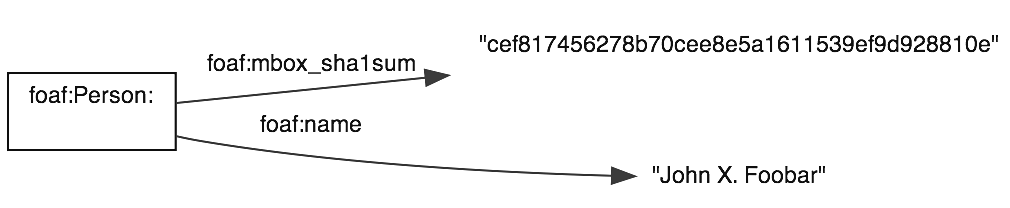
\includegraphics[width=\linewidth]{sample-rdf-graph.png} 
  \caption{Sample RDF graph visualized}
  \label{fig:sample-rdf-graph}
\end{figure}

\subsubsection{The RDF/XML Syntax}

RDF/XML~\cite{beckett2004rdfxml} was introduced by
the W3C as the first RDF serialization syntax.
Albeit more human-friendly serialization formats
such as Turtle~\cite{prudhommeaux2013turtle}
gain more and more traction,
RDF/XML is still very wide-spread.
Its media type is \texttt{application/rdf+xml},
the recommended file extension is \texttt{.rdf},
the encoding is UTF-8.
\autoref{code:rdfxml-syntax} shows the previously
introduced sample graph serialized in RDF/XML.

\begin{lstlisting}[caption={Sample graph in RDF/XML syntax},
  label={code:rdfxml-syntax}]
<?xml version="1.0" encoding="UTF-8"?>
<rdf:RDF
    xmlns:foaf="http://xmlns.com/foaf/0.1/"
    xmlns:rdf="http://www.w3.org/1999/02/22-rdf-syntax-ns#">
  <rdf:Description rdf:nodeID="node15urahancx74224">
    <rdf:type rdf:resource="http://xmlns.com/foaf/0.1/Person"/>
    <foaf:name>John X. Foobar</foaf:name>
    <foaf:mbox_sha1sum>
      cef817456278b70cee8e5a1611539ef9d928810e
    </foaf:mbox_sha1sum>
  </rdf:Description>
</rdf:RDF>
\end{lstlisting}

\subsubsection{The N-Triples Syntax} \label{sec:n-triples}

The N-Triples~\cite{grant2004ntriples} syntax was primarily
developed by Dave Beckett and Art Barstow.
N-Triples is a~subset of Turtle (see \autoref{sec:turtle}),
which in turn is a~subset of Notation3
(see \autoref{sec:notation3}).
There are very few variations to express a~graph in N-Triples,
which makes it an ideal syntax for testing purposes, however,
as it is missing some shortcuts of Turtle, it is quite verbose.
Its media type is \texttt{text/plain}, the recommended file extension is \texttt{.nt},
and the encoding is 7-bit US-ASCII
(and explicitly \emph{not} UTF-8).
\autoref{code:ntriples-syntax} shows the previously
introduced sample graph serialized in N-Triples.

\begin{lstlisting}[caption={Sample graph in N-Triples syntax},
  label={code:ntriples-syntax}]
_:1 <http://www.w3.org/1999/02/22-rdf-syntax-ns#type>
    <http://xmlns.com/foaf/0.1/Person> .
_:1 <http://xmlns.com/foaf/0.1/name>
    "John X. Foobar" .
_:1 <http://xmlns.com/foaf/0.1/mbox_sha1sum>
    "cef817456278b70cee8e5a1611539ef9d928810e" .
\end{lstlisting}

\subsubsection{The Turtle Syntax} \label{sec:turtle}

Turtle~\cite{prudhommeaux2013turtle},
or the Terse RDF Triple Language, was defined by Dave Beckett.
It is a~superset of N-Triples (see \autoref{sec:n-triples}) and
a~subset of Notation3 (see \autoref{sec:notation3}).
It has reached a~\emph{de~facto} standard status,
with the RDF Working Group publishing the new Turtle specification
as a~W3C Candidate Recommendation on February 19, 2013.
Its media type is \texttt{text/turtle}
(the sometimes still observable media type
\texttt{application/x-turtle} is deprecated),
the recommended file extension is \texttt{.ttl},
the encoding is UTF-8.
\autoref{code:turtle-syntax} shows the previously
introduced sample graph serialized in Turtle.

\begin{lstlisting}[caption={[Sample graph in Turtle syntax]{Sample graph in Turtle syntax,
  the syntax is equivalent to \autoref{code:notation3-syntax}}},
  label={code:turtle-syntax}]
@prefix foaf: <http://xmlns.com/foaf/0.1/> .

_:node15urahancx74223 a foaf:Person ;
  foaf:name "John X. Foobar" ;
  foaf:mbox_sha1sum "cef817456278b70cee8e5a1611539ef9d928810e" .
\end{lstlisting}

\subsubsection{The Notation3 Syntax} \label{sec:notation3}

Notation3~\cite{bernerslee2011notation3} was introduced
by Tim Berners-Lee.
Notation3 has some features that go beyond
the pure expressiveness of RDF like rules,
support for variables, and quantification.
Its media type is \texttt{text/n3},
the recommended file extension is \texttt{.n3},
the encoding is always UTF-8.
\autoref{code:notation3-syntax} shows the previously
introduced sample graph serialized in Notation3,
which, given the present trivial example,
is syntactically equal to Turtle.

\begin{lstlisting}[caption={Sample graph in Notation3 syntax},
  label={code:notation3-syntax}]
@prefix foaf: <http://xmlns.com/foaf/0.1/> .

_:node15urahancx74223 a foaf:Person ;
  foaf:name "John X. Foobar" ;
  foaf:mbox_sha1sum "cef817456278b70cee8e5a1611539ef9d928810e" .
\end{lstlisting}

\subsubsection{The RDFa Syntax}

RDFa~\cite{adida2012rdfa} has a~special role
in that it is a~specification for attributes
to express structured data in XHTML~\cite{pemberton2000xhtml},
but also in HTML4 and HTML5~\cite{sporny2012htmlrdfa}.
It uses the rendered hypertext content of (X)HTML
for the RDFa markup,
so that data publishers can use the same document
for human- and machine-readable content.
The contained RDF triples can be extracted with distillers.
In consequence, RDFa can be considered
another serialization syntax for RDF,
with the same expressive power as
RDF/XML~\cite{beckett2004rdfxml},
Turtle~\cite{prudhommeaux2013turtle}, \emph{etc.}
Its media type is \texttt{application/xhtml+xml},
the recommended file extension is \texttt{.html}.
RDFa shares some design goals
with Microformats~\cite{celik2006microformats}
and Microdata~\cite{hickson2012microdata}.
Where Microformats specify both a~syntax
for embedding structured data into HTML
\emph{and} a~vocabulary of specific terms for each Microformat,
RDFa in contrast \emph{only} specifies a~syntax,
since the vocabularies it relies on
are externally and independently specified.
The essence of RDFa is a~set of attributes
that contain metadata about things,
and that can be embedded in mark-up languages,
for example in XHTML or HTML.
The concrete attributes are as follows.

\begin{itemize}
  \item \texttt{about} and \texttt{src} a~URI or
        CURIE (compact URI)~\cite{birbeck2007curie}
        that specifies the resource
        the metadata is about.
  \item \texttt{rel} specifies a~relationship with
        another resource.
  \item \texttt{href} and \texttt{resource} specify
        the partner resource.
  \item \texttt{property} specifies a~property for
        the content of an element.
  \item \texttt{content} optional attribute that overrides
        the content of the element when using
        the property attribute.
  \item \texttt{datatype} optional attribute that
        specifies the datatype of text specified
        for use with the property attribute.
  \item \texttt{typeof} optional attribute that specifies
        the RDF type(s) of the subject (the resource
        that the metadata is about).
\end{itemize}

An additional simplified subset of RDFa is RDFa Lite~\cite{sporny2012rdfaalite}, which is aligned with Microdata.
\autoref{code:rdfa-syntax} shows the previously introduced
sample graph serialized in RDFa.

\begin{lstlisting}[caption={Sample graph in RDFa syntax},
  label={code:rdfa-syntax}]
<div about="_:1" typeof="http://xmlns.com/foaf/0.1/Person">           
  <span property="http://xmlns.com/foaf/0.1/mbox_sha1sum">
    cef817456278b70cee8e5a1611539ef9d928810e
  </span> 
  <span property="http://xmlns.com/foaf/0.1/name">
    John X. Foobar
  </span>
</div> 
\end{lstlisting}

\section{SPARQL: Semantic Web Query Language}

SPARQL is a~recursive acronym that stands for
SPARQL Protocol and RDF Query Language.
The SPARQL specification~\cite{prudhommeaux2008sparql}
defines the syntax and semantics
of the SPARQL query language for RDF.
RDF~\cite{klyne2004rdf} is a~directed, labeled
graph data format for representing information on the Web.
SPARQL can be used to express queries
across diverse data sources,
whether the data is stored natively as RDF,
or viewed as RDF via middleware.
SPARQL allows for querying required
and optional graph patterns
along with their conjunctions and disjunctions.
SPARQL also supports extensible value testing
and constraining queries by source RDF graph.
The results of SPARQL queries can be result sets or RDF graphs.
SPARQL became an official W3C Recommendation in 2008.
It was standardized by the RDF Data Access Working Group (DAWG).

\subsection{The Vision of the Web as a~Giant Single Database}

The Web as we know it today is a~\emph{network of documents},
interconnected by hyperlinks that everyone can participate in
by placing links to existing documents.
The vision of the Semantic Web, however,
is a~\emph{network of facts} about entities,
interconnected by means of graphs of data.
Where the Web of today is a~graph of documents,
the Semantic Web is envisioned to be a~huge global graph,
formed by many individual graphs.
If one party publishes facts about an entity
and a~different party publishes different facts
about the same entity,
then the overall knowledge about that entity
is represented in a~decentralized way,
accessible to all, and open for everyone to enrich.
This requires strong globally unique identifiers,
or at least ways to map one identifier to another.

Given the (visionary) huge global graph, a~fictive
SPARQL query like the one in \autoref{code:sparql}
could be used to get results from the graph,
like the email addresses of every person in the world.
SPARQL queries, unlike traditional databases, are not necessarily
guaranteed to return \emph{all} existing results (completeness).

\begin{lstlisting}[caption={[Fictive SPARQL query returning names and
  email addresses]
  {Fictive SPARQL query returning the names and email addresses of every
  person in the world
  (\url{http://en.wikipedia.org/wiki/SPARQL\#Benefits}, accessed July 15, 2013)}},
  label={code:sparql}]
PREFIX foaf: <http://xmlns.com/foaf/0.1/>
SELECT ?name ?email
WHERE {
  ?person a foaf:Person.
  ?person foaf:name ?name.
  ?person foaf:mbox ?email.
}
\end{lstlisting}

This query selects the names and email addresses from all persons
who have facts about them in the global graph.
The query starts with a~prefix definition,
and then constrains the results
to be of type \texttt{foaf:Person}~\cite{brickley2010foaf},
whose name and email address are the values
of the triples with the predicates \texttt{foaf:name}
and \texttt{foaf:mbox} respectively.
While this sounds like a~very powerful idea,
in practice SPARQL endpoints
like the DBpedia SPARQL
endpoint\footnote{\url{http://dbpedia.org/sparql}, accessed July 15, 2013}
typically only allow for querying a~local graph
for performance reasons.

\subsection{Different SPARQL Query Variations}

The SPARQL Query Language currently specifies four different query variants, which we will list in the following. 

\subsubsection{SELECT}

The \texttt{SELECT} query variant is used to extract
raw values from a~SPARQL endpoint.
The results are returned in a~tabular format.
A~sample query was given in \autoref{code:sparql}.

\subsubsection{DESCRIBE}

The \texttt{DESCRIBE} query variant is used to extract
an RDF graph from the SPARQL endpoint,
the contents of which is left to the endpoint to decide
based on what the maintainer deems as useful information.
An example query is given below:\\

\texttt{DESCRIBE <http://example.org/sparql>}

\subsubsection{ASK}

The \texttt{ASK} query variant is used to provide
a~simple \texttt{true} or \texttt{false} result
for a~query on a~SPARQL endpoint.
No information is returned about the possible query solutions,
just whether or not a~solution exists.
An example query with a~sample response is given below:\\

\noindent Given the RDF graph in \autoref{fig:sample-rdf-graph}
and the following SPARQL \texttt{ASK} query:\\

\texttt{PREFIX foaf: <http://xmlns.com/foaf/0.1/>\\
\indent ASK \{ ?x foaf:name  "Alice" \}}\\

\noindent This query creates the following response
(as there is no person named Alice in the graph,
but only a~person named John X. Foobar):\\

\texttt{no}

\subsubsection{CONSTRUCT}

The \texttt{CONSTRUCT} query variant is used to extract
information from the SPARQL endpoint
and to transform the results into valid RDF
specified by a~graph template.
The result is an RDF graph formed by taking
each query solution in the solution sequence,
substituting for the variables in the graph template,
and combining the resulting triples into
a~single RDF graph by set union.
An example query is given below.\\

\noindent Given the following RDF graph,
serialized in Turtle syntax:\\

\texttt{@prefix foaf: <http://xmlns.com/foaf/0.1/> .}\\
\texttt{\indent \_:a foaf:name "Alice" .}\\
\texttt{\indent \_:a foaf:mbox <mailto:alice@example.org> .}\\

\noindent Given the following SPARQL \texttt{CONSTRUCT} query:\\

\texttt{PREFIX foaf: <http://xmlns.com/foaf/0.1/>}\\
\texttt{\indent PREFIX vcard: <http://www.w3.org/2001/vcard-rdf/3.0\#>}\\
\texttt{\indent CONSTRUCT \{ <http://example.org/person\#Alice> vcard:FN ?name \}}\\
\texttt{\indent WHERE { ?x foaf:name ?name }}\\

\noindent This query creates the following
\texttt{vcard}~\cite{dawson1998vcard}
properties from the FOAF information:\\

\texttt{@prefix vcard: <http://www.w3.org/2001/vcard-rdf/3.0\#> .}\\ 
\texttt{\indent <http://example.org/person\#Alice> vcard:FN "Alice" .}

\section{Linked Data}

Linked Data~\cite{bernerslee2006linkeddata}
defines a~set of agreed-on best practices and
principles for interconnecting and publishing
structured data on the Web.
It uses Web technologies like HTTP~\cite{fielding1999http}
and URIs~\cite{bernerslee2005uri}
to create typed links between different sources.
The portal \url{http://linkeddata.org/} (accessed July 15, 2013)
defines Linked Data as being
\textit{``about using the Web to connect related data that
wasn’t previously linked, or using the Web
to lower the barriers to linking data
currently linked using other methods''}.

\subsection{The Linked Data Principles}
\label{sec:linked-data-principles}

Tim Berners-Lee defines the four rules for Linked Data in a~W3C Design Issue~\cite{bernerslee2006linkeddata} as follows:

\begin{enumerate}
  \item Use URIs as names for things.
  \item Use HTTP URIs so that people can look up those names.
  \item When someone looks up a~URI, provide useful information,
        using the standards (RDF*, SPARQL).
  \item Include links to other URIs,
        so that they can discover more things.
\end{enumerate}

Linked Data uses RDF~\cite{klyne2004rdf} to create
typed links between things in the world.
The result is oftentimes referred to as the \emph{Web of Data}.
As outlined before, RDF encodes statements
about things in the form of
\texttt{(subject, predicate, object)} triples.
If subject and object have URIs from different namespaces,
Bizer \emph{et~al.}\ speak of \emph{RDF links}
in~\cite{heath2011linkeddata}.
An exemplary RDF link adapted from~\cite{bizer2009linkeddatastory}
stating that a~description of the movie Pulp Fiction
from the Linked Movie Database~\cite{hassanzadeh2009linkedmovie}
and a~description from DBpedia~\cite{auer2007dbpedia}
are indeed talking about the same movie
can be seen in \autoref{code:rdflink}.

\begin{lstlisting}[caption={[Exemplary RDF link]{Exemplary RDF
  link stating that a~description of the movie Pulp Fiction from
  the Linked Movie Database~\cite{hassanzadeh2009linkedmovie}
  and a~description from DBpedia are indeed talking
  about the same movie}},
  label={code:rdflink},
  escapechar=§]
<http://data.linkedmdb.org/resource/film/77> §\linewrap§
  <http://www.w3.org/2002/07/owl#sameAs> §\linewrap§
  <http://dbpedia.org/page/Pulp_Fiction> .
\end{lstlisting}

\subsection{The Linking Open Data Cloud Diagram}
\label{sec:lodcloud}

The Linking Open Data (LOD) cloud
diagram~\cite{cyganiak2011lodcloud} is a~visualization effort
that shows datasets that have been published in
Linked Data~\cite{bernerslee2006linkeddata}
format by contributors to the Linking Open Data community project
and other individuals and organizations.
The objective is to identify existing datasets with open licenses,
convert them to RDF whilst obeying the Linked Data principles,
and finally publish them on the Web.
Due to its open structure, everyone can contribute to the project by publishing a~dataset and
interlinking it to existing datasets.
Today, the project includes datasets of major organizations
such as the BBC, Thomson Reuters, or the Library of Congress
to name just a~few.
The state of the LOD cloud has been examined
in~\cite{bizer2011statelodcloud}.
The latest LOD cloud diagram as of September 2011 can be seen in \autoref{fig:lod-cloud}.

\begin{figure}[!ht]
\centering  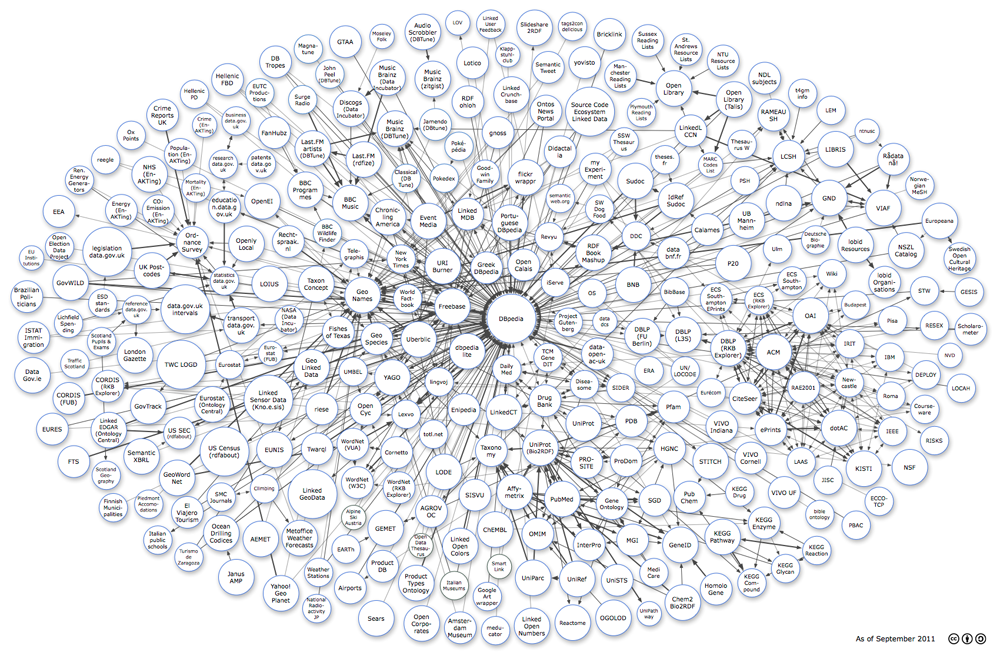
\includegraphics[height=0.8\textheight,keepaspectratio]{lod-cloud.png}    
  \caption[Linking Open Data cloud diagram as of September 2011]
  {Linking Open Data cloud diagram as of September 2011, by Richard Cyganiak and Anja Jentzsch \url{http://lod-cloud.net/} (accessed July 15, 2013) \todo{Check final orientation}}    
  \label{fig:lod-cloud}
\end{figure}

\section{Conclusions}

In this chapter, we have first introduced the Semantic Web
and compared it to the non-semantic Web.
We have shown how structured data in the form of tables
is a~first step towards richer semantics.
An example of converting structured data from Wikipedia
into machine-readable data is the knowledge base DBpedia.
Further, we have looked at the intrinsic semantics
of HTML in versions 4 and 5,
and how through additional attributes
even richer semantics can be added
by the annotation formats Microdata and Microformats.
We have introduced the Resource Description Format (RDF)
and its different serializations.
On top of RDF, we have detailed
how the Semantic Web query language SPARQL
can be used to express queries across data sources.
Finally, we have shown how data on the Web
can be exposed as so-called Linked Data,
an effort which is visualized in the Linking Open Data cloud.
By introducing these Semantic Web technologies,
we have set the foundations for the coming chapters
that build upon those pillars.

\section*{Chapter Notes}
This chapter is partly based on the following publications:
\todo{Add publications}

\bibliographystyle{plainnat}
\clearpage
\bibliography{backmatter/references}

\chapter{Social Networks}
\label{cha:social-networks}

% the code below specifies where the figures are stored
\ifpdf
    \graphicspath{{3_social_networks/figures/PNG/}{3_social_networks/figures/PDF/}{3_social_networks/figures/}}
\else
    \graphicspath{{3_social_networks/figures/EPS/}{3_social_networks/figures/}}
\fi

From the first ever email to video calls on the go,
the Internet has always been about communication.
Historically, communities formed around Usenet mailing lists or Bulletin Board Systems, starting from the early eighties,
often around all sorts of topics like fine arts,
literature, and philosophy (\emph{e.g.}, \texttt{humanities.classics}
or \texttt{humanities.\-design.misc}).
Then, starting from the late eighties, Internet Relay Chats (IRC)
allowed people to communicate interactively and in real-time,
organized in channels (\emph{e.g.}, \texttt{\#linux}).
Starting from the nineties, blogs began to spread,
reaching mainstream popularity somewhere in mid-2000.
While the early social communities
where created entirely \emph{ad-hoc}
whenever someone logged in to a~system,
the first social networks,
among them \url{http://sixdegrees.com/} in 1997,
allowed people to maintain a~public profile
with a~list of connections (\emph{friends})
that others could browse.
In~\cite{boyd2007socialnetworksites}, boyd
(\emph{sic}\footnote{http://www.danah.org/name.html})
and Ellison define the term
\emph{social network site (SNS)} as follows.

\begin{quotation}
  \textit{``We define social network sites as web-based services
  that allow individuals to
  (1) construct a~public or
  semi-public profile within a~bounded system,
  (2) articulate a~list of other users
  with whom they share a~connection, and
  (3) view and traverse their list of connections
  and those made by others within the system.
  The nature and nomenclature of these connections
  may vary from site to site.''}
\end{quotation}

Literature on social networks oftentimes uses the term SNS,
however, in order to differentiate ourselves
from the therein defined idea of social network,
we decided to avoid the term altogether in favor of a~more open
definition of social network,
which we detail in the following. 

\section{Definition of Terms Used in this Thesis}
\label{sec:definition}

In this section, we define the terms
that we will use throughout this thesis
in order to avoid any ambiguity.
In particular, we highlight that social networks have
different levels of support for media items.

\begin{description}
  \item[Social Network:]
       A~social network is an online service or media platform
       that focuses on building and reflecting
       relationships among people
       who share interests and/or activities.
  \item[Media Item:]
       A~media item is defined as
       a~photo\footnote{We chose the term \emph{photo}
       over the term \emph{image} as 
       Facebook, Twitter, and \googleplus use it.}
       or video
       file that gets distributed via a~social network.
  \item[Micropost:]
       A~micropost is defined as a~textual status message
       that can optionally be accompanied by a~media item.
  \item[Hashtag] The \texttt{\#} symbol, called a~hashtag,
       is used to mark keywords or topics in a~micropost.
       It was created organically by Twitter users
       as a~way to categorize messages.
       People use the hashtag symbol \texttt{\#} before a~relevant keyword
       or phrase (no spaces) in microposts to categorize them
       and help them show more easily in
       search\footnote{Adapted from
       \url{https://support.twitter.com/articles/49309-what-are-hashtags-symbols},
       accessed December 7, 2012.}. 
\end{description}

The boundary between \emph{social networks} and
\emph{media platforms} is blurred.
Several media sharing platforms, \emph{e.g.},
YouTube\footnote{http://youtube.com/},
enable people to upload content
and optionally allow other people to react
to this content in the form of comments, likes or dislikes.
On other social networks, \emph{e.g.},
Facebook\footnote{http://facebook.com/},
users can update their status, post links to stories,
upload media content, and also give readers the option to react.
Finally, there are hybrid clients, \emph{e.g.},
TweetDeck\footnote{http://www.tweetdeck.com/}
by Twitter together with
Twitpic\footnote{http://twitpic.com/},
where social networks integrate with media platforms,
typically via third-party applications.

\section{Description of Popular Social Networks}
\label{sec:description-of-popular-social-networks}

In this section, we introduce several social networks
and some of their key features
that are relevant for our approach.
As we treat all networks the same---%
independent from their not always publicly known user population---%
they are listed in alphabetic order.
For active participation,
all social networks require users to be logged in.
In the description below, we thus assume a~logged in user.

\subsection{Facebook}

Facebook (\url{http://www.facebook.com/})
is a~social networking service launched in February 2004,
operated and owned by the American multinational
Internet corporation Facebook, Inc.
At time of writing, Facebook is the most popular social network
with one billion monthly active
users\footnote{\url{http://newsroom.fb.com/Key-Facts},
accessed November 19, 2012}
as of October 2012.
Facebook has native photo and video support,
allowing people to upload an unlimited amount of media items.
Photos and videos can also be recorded \emph{ad hoc} via webcam.
People can \emph{Like} content via a~designated Like button
that can also be embedded on other websites.
Initially, the button was called the \emph{Awesome} button,
but eventually\footnote{\url{http://www.quora.com/Facebook-Inc-company/Whats-the-history-of-the-Awesome-Button-that-eventually-became-the-Like-button-on-Facebook}}
got rebranded to its current form.
Individual microposts can also be shared.
Facebook has a~bidirectional relationship model (friend model),
with an optional unidirectional relationship model (follow model),
typically for following celebrities, remote friends, \emph{etc.}

\subsection{Flickr}

Flickr (\url{http://www.flickr.com/})
is a~photo and video hosting online community
created by Ludicorp in 2004 and acquired by Yahoo! in 2005.
Users can upload a~limited or unlimited number of photos or videos
to the service, depending on their account type (Free or Pro).
People can \emph{Favorite} photos they like
via a~designated Favorite button.
Flickr has a~unidirectional relationship model (follow model),
however, also allows people to mark other users as friends
or family \emph{without} the other party having to confirm.
Following an urgent plea from Flickr
users\footnote{\url{http://dearmarissamayer.com/}},
where they complained that Yahoo!
had semi-abandoned the service for too long,
Flickr is now said to be revived under new CEO Marissa
Mayer\footnote{\url{http://www.flickr.com/dearinternet}}.

\subsection{\googleplus}

\googleplus (\url{http://google.com/+}),
sometimes transcribed as Google Plus
and abbreviated as \gplus, is Google's social network.
It was opened to the general public on September 20, 2011.
\googleplus has native photo support.
Photos can either be manually uploaded
when authoring a~new micropost,
or be automatically uploaded via the \googleplus
mobile application.
External videos, for example, from
the also Google-owned online video platform YouTube,
but also from other services,
get displayed in an inline view
so that they can be viewed directly on the website.
However, the network also allows for
videos to be uploaded directly,
or to be recorded \emph{ad hoc} via webcam.
People can \emph{\plusone}
(pronounced like a~verb ``to plus-one'') content they like
via a~designated \plusone button
that can also be embedded on other websites.
Individual microposts can also be shared.
\googleplus has a~unidirectional relationship model
(follow model).

\subsection{Img.ly}

Img.ly (\url{http://img.ly/})
is a~photo hosting service operated by 9elements GmbH
and founded in 2009.
It integrates deeply with Twitter, however,
can also be used independently.
Img.ly integrates with Twitter's \emph{Tweet} button. 
The service has no own relationship model,
but uses a~user's social graph on Twitter.

\subsection{Imgur}

Imgur (\url{http://imgur.com/})
is a~photo hosting service
founded by Alan Schaaf in February 2009.
While the service is deeply integrated with Twitter
and Facebook, it can be used independently as well.
Imgur integrates with all major social networks,
and also has designated \emph{Like} and \emph{Dislike} buttons.
The service has no own relationship model,
but uses a~user's social graph on Facebook.

\subsection{Instagram}
\label{sec:instagram}

Instagram (\url{http://instagram.com/})
is a~mobile photo sharing application
that was acquired by Facebook in April 2012.
The application allows users to apply filters to photos.
These photos can then be shared on external social networks
like Facebook, Twitter, or \googleplus,
and are also visible on Instagram's own social network.
The service launched in October 2010.
Instagram has native photo support, but,
does not support videos.
People can \emph{Like} content via a~designated Like button
from within the Instagram application.
Instagram has a~unidirectional relationship model (follow model).

\subsection{Lockerz}

Lockerz (\url{http://lockerz.com/}) is an international
social commerce website based in Seattle, WA. 
In 2011, Lockerz acquired the photo sharing service Plixi,
whih was formerly known as TweetPhoto.
Lockerz keeps Plixi's service as a~media platform running
under the new Lockerz branding.
While the service is deeply integrated with Twitter,
it can be used independently as well.
People can \emph{Love} content they like via
a~designated Love button,
but the service is also integrated with all major social networks.

\subsection{MobyPicture}

MobyPicture (\url{http://www.mobypicture.com/})
is a~mobile messaging service
owned by entrepreneur Mathys van Abbe.
Users of the service can upload an unlimited number of
photos and videos to the service.
MobyPicture integrates with a~number of
third-party social networks.
The service natively supports videos and photos,
which can either be uploaded, or be recorded \emph{ad hoc}
via webcam.
People can \emph{Favorite} content they like via
a~designated Favorite button,
however, the service also integrates with Google's
\emph{\plusone} button and Twitter's \emph{Tweet} button. 
MobyPicture has a~unidirectional relationship model
(follower model).

\subsection{Myspace}

Myspace (\url{http://www.myspace.com/}),
formerly MySpace and My\_\_\_\_\_ (\emph{sic}), is
a~social networking service owned by Specific Media LLC
and pop star Justin Timberlake.
The social network launched in August 2003.
Once the most visited website
in the United States in June 2006,
the network's importance is steadily declining since.
Instead of as a~social networking website,
Myspace has attempted to redefine itself
as a~social entertainment website,
putting more focus on music, movies, celebrities, and TV.
At time of writing, yet another redefinition process is
ongoing\footnote{\url{https://new.myspace.com/}}.
As such, Myspace has native photo, video, and,
via special musician profiles, audio support.
Videos can either be uploaded,
or be recorded \emph{ad hoc} via webcam.
In January 2012, a~rebranding strategy to Myspace TV
in collaboration with Panasonic was unveiled
with an exclusive focus on social TV that would allow people
to watch and comment on videos.
People can \emph{Like} certain content via a~designated Like link.
Myspace has a~bidirectional relationship model (friend model),
with an optional unidirectional relationship model (follow model),
typically meant for following celebrities like artists,
musicians, \emph{etc.}

\subsection{Photobucket}

Photobucket (\url{http://photobucket.com/})
is a~photo and video hosting service
founded in 2003 by Alex Welch and Darren Crystal.
It was acquired by Fox Interactive Media in 2007.
In June 2011, Twitter announced an exclusive partnership
with Photobucket that made the service
the default photo sharing platform for Twitter,
used for its native media item support.

\subsection{Twitpic}

Twitpic (\url{http://twitpic.com/})
is a~service that allows users to upload photos and videos.
It optionally integrates with Twitter.
Twitpic was launched in 2008 by Noah Everett.
While Twitpic can be used independently from Twitter,
the integration is made easy with Twitpic usernames and passwords
being the same as the ones on Twitter.
Twitpic integrates with Twitter via the \emph{Tweet} button.
The service has no own relationship model,
but uses a~user's social graph on Twitter.

\subsection{Twitter}
\label{sec:twitter}

Twitter (\url{http://twitter.com/})
is an online social networking service
and microblogging service
that enables its users to send and read microposts
of up to 140 characters.
These microposts are referred to as \emph{tweets}.
Twitter was founded in March 2006 by Jack Dorsey
and launched to the public in July 2006.
The website is ranked among the top-10 websites globally
by the Web information company
Alexa\footnote{\url{http://www.alexa.com/topsites},
accessed November 19, 2012}.
As of August 2011, Twitter has native photo support,
which allows users to upload photos to the service.
However, at time of writing, it is not possible to 
record photos or videos \emph{ad hoc} via webcam.
Videos are not supported natively, however,
likewise the situation with photos before
(and also in part still today),
an ecosystem of media platforms takes care of
hosting media items on behalf of Twitter users.
These third-party-hosted media items
can be linked from within tweets.
People can \emph{ReTweet} content they like either
via a~designated ReTweet button,
or---following the prior, but still widely popular,
manual ReTweet convention---by
quoting a~Twitter user by prepending ``RT @username:''
in front of the original tweet.
In addition to that, Twitter offers
a~\emph{Tweet} button that can be embedded on other websites.
Twitter has a~unidirectional relationship model (follow model).

\subsection{Yfrog}

Yfrog (\url{http://yfrog.com/})
is a~photo and video hosting service run by ImageShack
that was launched in February 2009.
While the service is deeply integrated with Twitter,
it can be used independently as well.
Yfrog integrates with Twitter's \emph{Tweet} button.
The service has no own relationship model,
but uses a~user's social graph on Twitter.

\subsection{YouTube}

YouTube (\url{http://www.youtube.com/})
is a~video sharing website founded in February 2005.
In November 2006, YouTube was acquired by Google,
and now operates as a~subsidiary of the company.
It allows people to upload, view,
and share an unlimited number of videos.
YouTube has native video support, but, does not support photos.
Videos can be uploaded, or be recorded \emph{ad hoc} via webcam.
People can \emph{Like} or \emph{Dislike} content
via designated Like or Dislike buttons.
YouTube has a~unidirectional relationship model (follow model).

\section{Decentralized Social Networks}
All social networks presented up to now are centralized networks.
In contrast, \emph{distributed}, or also referred to as
\emph{decentralized social networks}, are
social network services that are decentralized and distributed
across different providers, with a~special focus on
portability, interoperability, and federation capability,
\emph{i.e.}, an agreement upon standards of operation
in a~collective fashion.
Decentralized, protocol-based systems
offer users a~choice of providers, which implies
that, if one provider should terminate their service,
the user is free to take out her data and start
where she left off with a~different provider.
As a~final advantage, governments cannot effectively censor
decentralized social networks,
as this would be impracticable due to the distributedness.

\subsection{Examples of Decentralized Social Networks}

In the following, we will list representative efforts 
in the direction of truly decentralized social networks.
This list is not meant to be complete,
but covers the efforts that received the most media attention
in the years 2011 and 2012.

\subsubsection{StatusNet}

A~first example of decentralized social network software providers
is StatusNet ({\url{http://status.net/}),
which provides an open-source implementation of the
OStatus\footnote{\url{http://gitorious.org/projects/ostatus/}}
open standard, most prominently deployed
at \url{http://identi.ca/}.

\subsubsection{The DIASPORA* Project}

A~second example is the DIASPORA* project (\url{http://diasporaproject.org/}),
which provides a~free and open-source personal Web server component
referred to as \emph{pod} that allows
participants in the project to form nodes
that span the distributed Diaspora social network.

\subsubsection{Tent}

Third, there is Tent\texttrademark~(\url{https://tent.io/}).
Tent is an open-source protocol for distributed social networking
and personal data storage.
Anyone can run a~Tent server,
or write an app or alternative server implementation
that uses the Tent protocol.
Users can take their content and relationships with them
when they change or move servers.
Tent supports extensible data types,
so developers can create new kinds of interactions.
Rather than running an own server,
users can also rely on Tent.is (\url{https://tent.is/}),
a~service which hosts Tent servers
and basic applications for users.
Yet the global site feed\footnote{\url{https://app.tent.is/global}},
suggests that the service is not very active.

\subsection{Current Status of Decentralized Social Networks}

None of the decentralized social networks could reach
a~critical mass of users and/or network activity as of yet.
We will therefore not consider them for this thesis.

\section{Classification of Social Networks}
\label{sec:classification-of-social-networks}

As motivated in \autoref{sec:definition},
different social networks have varying support
for media items, ranging from native support
in media-centric social networks,
to optional support in micropost-centric social networks.
In order to differentiate social networks by their
media item support level,
we introduce a~classification of social networks as follows.

\begin{itemize}
  \item \emph{First-order support}:
        The social network is centered around media items
        and posting requires the inclusion of a~media item
        (\emph{e.g.}, YouTube, Flickr).
  \item \emph{Second-order support}:
        The social network lets users upload media items,
        but it is also possible to post purely textual messages
        (\emph{e.g.}, Facebook).
  \item \emph{Third-order support}:
        The social network has no direct support for media items,
        but relies on third-party media platforms
        to host media items, which are linked to the status update
        (\emph{e.g.}, Twitter relying on third-party video hosting via Twitpic).
\end{itemize}

In this chapter, we consider 11 different social networks
that represent all together most of the market share.
The criteria for inclusion follow
a~study~\cite{levine2011howpeopleshare}
performed by the company Sysomos, specialized in social media
monitoring and analytics.
\autoref{tab:platforms} lists these social networks according to the categorization defined above.

\begin{sidewaystable}
  {\small
  \begin{tabular}{|l|l|l|p{8cm}|}
    \hline
    \textbf{Social Network} & \textbf{URL} & \textbf{Category} & \textbf{Comment}\\
    \hline
	\googleplus & \url{http://google.com/+} & second-order & Media item links are returned via the \googleplus API.\\
	Myspace & \url{http://myspace.com} & second-order & Media item links are returned via the Myspace API.\\
	Facebook & \url{http://facebook.com} & second-order & Media item links are returned via the Facebook API.\\
	Twitter & \url{http://twitter.com} & second-/third-order & In second order mode, media item links are returned via the Twitter API. In third order mode, Web scraping or media platform API usage are necessary to retrieve media item links. Many people still use Twitter in third order mode.\\\hline
	Instagram & \url{http://instagram.com} & first-order & Media item links are returned via the Instagram API.\\
	YouTube & \url{http://youtube.com} & first-order & Media item links are returned via the YouTube API.\\
	Flickr & \url{http://flickr.com} & first-order & Media item links are returned via the Flickr API.\\
	MobyPicture & \url{http://mobypicture.com} & first-order & Media platform for Twitter. Media item links are returned via the MobyPicture API.\\
	Twitpic & \url{http://twitpic.com} & first-order & Media platform for Twitter. Media item links are returned via the Twitpic API.\\
	Img.ly & \url{http://img.ly} & first-order & Media platform for Twitter. Media item link must be retrieved via Web scraping.\\
	Yfrog & \url{http://yfrog.com} & first-order & Media platform for Twitter. Media item links must be retrieved via Web scraping.\\
	\hline
  \end{tabular}
  }
  \caption[11 social networks with different level of support for media items]
  {11 social networks with different level of support for media
   items and techniques needed to retrieve them. \todo{Check final orientation}}
  \label{tab:platforms}  
\end{sidewaystable}

\section{Conclusions}
Alongside the Semantic Web background technologies
that were introduced in the previous chapter,
social networking sites form the backbone of this thesis.
In this chapter, we have thus first defined the terms of
\emph{social network}, \emph{micropost}, \emph{media platform},
and \emph{media item}.
Subsequently, we have introduced and described in detail
the most popular social networking sites and media platforms.
Different social networking sites have
a~different level of support for media items.
We have therefore classified the social networking site
landscape accordingly.
In the upcoming chapters, we will get to the core of
micropost annotation, media item extraction from microposts,
followed by media item deduplication, clustering, and ranking.
Finally, we will close the core part with media item compilation.

\section*{Chapter Notes}
This chapter is partly based on the following publications:
\todo{Add publications}

\bibliographystyle{plainnat}
\bibliography{backmatter/references}

\chapter{Micropost Annotation}
\label{cha:micropost-annotation}

% the code below specifies where the figures are stored
\ifpdf
    \graphicspath{{4_micropost_annotation/figures/PNG/}{4_micropost_annotation/figures/PDF/}{4_micropost_annotation/figures/}}
\else
    \graphicspath{{4_micropost_annotation/figures/EPS/}{4_micropost_annotation/figures/}}
\fi

\section{Introduction}

Microposts are the textual metadata that accompany media items.
\emph{Per~se}, these microposts are nothing but strings.
For the task of making sense out of social network microposts,
our contributions are methods to consolidate and rank
the results of multiple named entity recognition and
disambiguation Web services that we have unified in form
of a~wrapper Web service that (i) takes care of both
consolidation and ranking, and that
(ii) transparently tracks the underlying Web services'
data provenance.

The impact of social networks is ever-growing.
According to official statistics, Facebook is the biggest
social network with one billion monthly active
users\footnote{\url{http://newsroom.fb.com/Key-Facts},
accessed July 15, 2013}
as of October 2012.
Official user statistics from
Twitter\footnote{\url{http://blog.twitter.com/2012/03/twitter-turns-six.html},
accessed July 15, 2013}
stemming from March 2012 suggest
that currently more than 140 million active users
share 340 million tweets a~day.
Altogether, the users of social networks
produce an incredible amount of public and private data.
In this chapter, we thus report on methods to access and make sense
out of \emph{public} status updates,
or, our preferred term, microposts.

\subsection{Direct Access to Micropost Raw Data}

Social networks in general offer so-called
Application Programming Interfaces (APIs)
in order to allow for developers to access
part of the networks' data programmatically.
Similar to the microblogging site Twitter
with its search
API,\footnote{\url{https://dev.twitter.com/docs/api/1.1/get/search/tweets},
accessed July 15, 2013}
Facebook offers both a~search function on the website
and a~search
API,\footnote{\url{https://developers.facebook.com/docs/reference/api/},
accessed July 15, 2013}
and so does
\googleplus.\footnote{\url{https://developers.google.com/+/api/},
accessed July 15, 2013}
In order to perform data mining,
a~statistically significant amount of microposts is necessary.
Having access to \emph{all} microposts of a~service is referred to as
having access to the \emph{fire hose}.
Typically, developers are only granted access to a~smaller random 
sample of microposts (colloquially referred to as \emph{garden hose} access).
While Twitter grants all developers \emph{garden hose} access to its Streaming
APIs,\footnote{\url{https://dev.twitter.com/docs/streaming-apis},
accessed July 15, 2013}
for Facebook and \googleplus there are no such documented options.

\subsection{Browser Extensions to Access Microposts Indirectly}

To address this shortage, we have developed browser extensions
for the two major social networks Facebook and Twitter
called Facebook Swarm
NLP\footnote{\url{http://bit.ly/facebookswarmnlp},
accessed July 15, 2013}
and Twitter Swarm
NLP\footnote{\url{http://bit.ly/twitterswarmnlp},
accessed July 15, 2013}
that can be added to a~popular Web browser.
These extensions inject JavaScript code into Facebook and
Twitter to perform data analysis on the encountered set of
\emph{public} microposts by sending extracted data
to a~central data processing unit.
Users need to be logged in to Facebook or Twitter for the 
extensions to work and must have given
their \emph{explicit agreement} during
the extension installation process
for part of their data to be shared in an anonymized way.
While this is far inferior and not comparable
with direct \emph{fire hose} access,
given a~critical amount of participants,
it still provides access to a~random sample of microposts
from different social networks.

\subsection{Data Analysis Flow}

The extensions first retrieve all status updates
from the contacts that are displayed
on the current user's timeline.
Second, the extensions perform named entity extraction (NEE)
and disambiguation via Natural Language Processing (NLP)
using a~remote NLP API on each of the microposts
in order to add semantic meaning to them.
The extracted named entities are then displayed
along each micropost, as illustrated in \autoref{fig:facebookswarmnlp}.
Finally the extracted named entities
are sent to a~central Web analytics framework~\cite{kaushik2009analytics}
to compute basic or advanced trends, for example,
by ranking the most discussed named entities per day,
or by pivoting named entities by Web analytics data,
like users' geographic locations.

\begin{figure}[!ht]
  \centering
  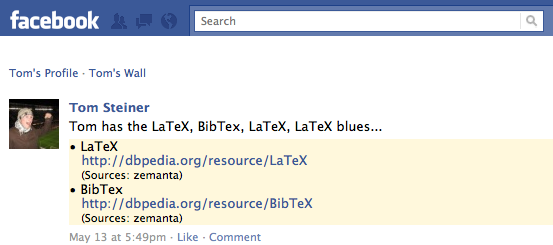
\includegraphics[width=0.75\textwidth]{facebook-swarm-nlp.png}
  \caption[Facebook Swarm NLP browser extension]
    {Facebook Swarm NLP browser extension.
    Extracted named entities have a~pale yellow background.}     
  \label{fig:facebookswarmnlp}
\end{figure}

\subsection{A~Wrapper API for Named Entity Disambiguation}
\label{sec:wrapperapi}

As mentioned before, in order to perform named entity extraction
and disambiguation, we rely on a~wrapper API
that calls existing third-party NLP APIs in the background
and that delivers the combined results of these APIs
in a~consolidated way.
It is  desirable
(i)~to credit back the contribution of each single third-party API
to the joint results, and
(ii)~to track the provenance of the joint results
in order to understand how they were formed.
We will show how these two constraints
can be fulfilled in a~generalizable way
at the concrete example of the wrapper NLP API
used for our browser extensions.

\section{Related Work}

We regard related work from different angles.
First, we look at different approaches
for named entity disambiguation,
which are relevant for adding meaning to microposts.
Second, we look at efforts to mash-up Web services,
which is important for tracking data provenance
when using multiple APIs in combination.

\subsection{Named Entity Disambiguation Using Lexical Databases}

In~\cite{choudhury2009youtubetags},
Choudhury \emph{et~al.}\ describe a~framework for
the semantic enrichment, ranking, and integration
of Web video tags using Semantic Web technologies.
This task is more related to microposts
than it seems at first sight:
video tags can consist of more than one word
and microposts (especially on Twitter) oftentimes consist
of just a~few words.
In order to enrich the typically sparse
user-generated tag space,
metadata like the recording time and location
or the video title and video description are used,
but also social features such as the playlists
where a~video appears in and related videos.
Next, the tags are ranked by their co-occurrence
and in a~final step interlinked with DBpedia~\cite{auer2007dbpedia}
concepts for greater integration with other datasets.
The authors disambiguate the tags based on
WordNet~\cite{miller1995wordnet,fellbaum1998wordnet}
synsets (groups of data elements that are considered
semantically equivalent for the purpose of information retrieval)
if possible, \emph{i.e.},
if there is only one matching synset in WordNet,
the corresponding WordNet URI in DBpedia is selected.
If there are more than one matching synsets,
the tags' and their context tags' similarity is computed
to decide on an already existing tag URI.

\subsection{Named Entity Disambiguation with Semantic Coherence and News Trends}

In~\cite{fernandez2007identityrank},
Fernández \emph{et~al.}\ examine named entity disambiguation
in the context of news annotation.
Their approach consists of three steps:
finding the candidate instances in the NEWS
ontology~\cite{fernandez2010newsontology}
for each entity in a~news item,
ranking these candidate instances
using a~modified version of
PageRank~\cite{brin1998pagerank},
and finally retraining the algorithm
with the journalist's feedback once the process is finished.
The approach first takes into account the number
of occurrences of candidate entities in the past
in order to find news trends,
and second, the occurrences of candidate entities
in past articles in the same categories
in order to find semantic coherences.

\subsection{Named Entity Disambiguation with Disambiguation Dictionaries}

In~\cite{nguyen2008namedentity},
Nguyen \emph{et~al.}\ show how disambiguation dictionaries
can be used to disambiguate entities
using Wikipedia disambiguation pages.
For a~set of entity candidates, all disambiguations are ranked
using tf-idf (or cosine similarity)~\cite{manning2008ir}.
The approach is a~hybrid and incremental process
that utilizes previously identified named entities
and related terms co-occurring with ambiguous names
in a~text for entity disambiguation.

\subsection{Disambiguation with Corpuses and Probability}

Cucerzan shows in~\cite{cucerzan2007largescale}
the use of a~corpus like Wikipedia for entity disambiguation.
The surrounding words of the to-be-disambiguated terms
plus the tags and categories of the related Wikipedia articles
are used to determine semantic coherence and thus
to decide on the most probable entity candidate.
This happens through a~process of heuristically maximizing
the agreement between contextual information
extracted from Wikipedia and the context of a~document.

\subsection{Disambiguation With Search Query Logs}

In~\cite{billerbeck2010rankingentities}, Billerbeck \emph{et~al.}\ use
click graphs and session graphs
of users' search engine sessions
to semantically bridge different queries in order to
retrieve entities for a~concrete entity retrieval query.
Click graphs are created by using queries and URLs as nodes
and connecting and weighting them by their click frequencies.
Session graphs are created by using only queries as nodes
with edges between them if they appear in the same user sessions,
again weighted by co-occurrence frequencies.
An exemplary entity retrieval query is \emph{hybrid cars},
semantically bridgeable queries are consequently \emph{toyota prius},
or \emph{honda civic hybrid}).
These entities are then ranked and returned to the user.

\subsection{Combining Different Web Services and Provenance}

In~\cite{groth2009mashups}, Groth \emph{et~al.}\ describe
how so-called mash-ups can be created in a~dynamic,
just-in-time way, combining data from different data sources
through tools and technologies such as
Yahoo! Pipes,\footnote{\url{http://pipes.yahoo.com/pipes/},
accessed July 15, 2013}
RSS~\cite{cadenhead2006rss}, and APIs.
The authors are driven by the motivation to allow for trust
and confidence in mash-ups, and therefore
consider it critical to be able to analyze the origin
of combined results.
They suggest an approach based on OWL~\cite{mcguinness2004owl}
and XML~\cite{bray2008xml},
with a~focus on process documentation.
However, different from our work, where the goal is to transparently
add provenance data at API invocation time,
their focus is more on overall process documentation
in the context of a~mash-up application.

The focus of Carroll \emph{et~al.}\ in~\cite{carroll2005namedgraphs}
is on the provenance of triples in the Semantic Web world, namely,
for making statements about triples in graphs.
Therefore, the authors introduce the concept of Named Graphs,
an extension to RDF~\cite{klyne2004rdf}.
In contrast to our work, Carroll \emph{et~al.}\ focus
purely on using triples to make statements about triples
(\emph{i.e.}, stay in the RDF world),
whereas our approach uses RDF to make statements
about potentially any API result.
 
Web service specifications in the context of the 
first-generation standards represented by WSDL~\cite{christensen2001wsdl},
SOAP~\cite{gudgin2007soap}, and UDDI~\cite{sabbouh2001uddi}
are occasionally referred to collectively as \emph{WS-*}.
In the \emph{WS-*} world, BPEL4WS, described by
Curbera \emph{et~al.}\ in~\cite{curbera2003bpel4ws}
provides a~formal language for the specification of
business processes and business interaction protocols.
This allows for the combination of several APIs.
However, it does not credit back concrete outputs of a~combined API
to the underlying APIs.

\section{Structuring Unstructured Textual Data} 
\label{sec:structuring}

When we speak of adding structure to unstructured textual data,
we mean the process of extracting the main concepts
in the form of named entities from a~given text
and the process of disambiguating those named entities,
\emph{i.e.}, the removal of uncertainty of meaning from
an ambiguous named entity like \emph{Barcelona},
which can stand for the football club, or the city of Barcelona.
An \emph{entity} is defined by
WordNet~\cite{miller1995wordnet,fellbaum1998wordnet}
as \textit{``that which is perceived or known or inferred
to have its own distinct existence (living or nonliving)''}. 
Typically, named entities from a~text can be persons, companies,
organizations, geographies, but also things like quantities,
expressions of time, books, albums, authors, \emph{etc.}
The extraction of named entities is commonly based on
Natural Language Processing (NLP) combined with Machine Learning.

\subsection{Natural Language Processing Services}
\label{sec:nlp-services}

WordNet~\cite{miller1995wordnet,fellbaum1998wordnet}
defines \emph{Natural Language Processing} as
\textit{``the branch of information science that deals with
natural language information''}.
From the many NLP toolkits available,
hereafter, we list some NLP Web services
that link to datasets in the
Linking Open Data
cloud~\cite{bizer2011statelodcloud,cyganiak2011lodcloud}
in order to disambiguate named entities.

\subsubsection{OpenCalais}\label{sec:opencalais}

The OpenCalais%
\footnote{\url{http://www.opencalais.com/documentation/opencalais-documentation},
accessed July 15, 2013}
Web service automatically creates rich semantic metadata
for textual documents.
Using Natural Language Processing (NLP),
machine learning, and other methods, OpenCalais analyzes documents
and finds the entities within, and also returns the facts and
events hidden within them.
OpenCalais is the only of the examined Web services
that provides details on occurrences in concrete sections
of the submitted coherent text.
This allows for the exact matching of the location in the text
where a~certain entity is detected.
This is especially useful as OpenCalais
is also oftentimes capable of recognizing references
within the text to prior discovered entities
(for example, in the following text,
\emph{he} is mapped back to Obama: \textit{``\emph{Obama}
thanked people for their work in ensuring the victory.
\emph{He} also thanked his family.''}).
An OpenCalais response consists of three parts:

\begin{itemize}
  \itemsep0em
  \item a~list of topics that the text is categorized in
  \item a~list of concrete entities that occur in the text
  \item a~list of social concept tags
\end{itemize}

The problem with the extracted entities is
that they are not always uniquely disambiguated.
An example is the named entity
represented by the URL \url{http://d.opencalais.com/pershash-1/cf42394f-4ae9-3e8e-958a-088149c86565.html}
that represents the concept of an entity of type \texttt{person}
named \emph{Barack Hussein Obama}.
However, a~\texttt{person}-type \emph{Barack Obama} entity from the same document is also represented by the URL
\url{http://d.opencalais.com/pershash-1/cfcf1aa2-de05-3939-a7d5-10c9c7b3e87b.html}
Other services successfully disambiguated both occurrences and
recognized them to stand for the same person, President Obama.
A~second issue is that only a~tiny fraction of the returned
entities link to other data sources in the
LOD cloud~\cite{bizer2011statelodcloud,cyganiak2011lodcloud}.
In order to discover links to the LOD cloud,
each returned entity URL has to be retrieved at the expense
of an HTTP request and the returned RDF has to be checked
for said links.

\subsubsection{AlchemyAPI}

AlchemyAPI\footnote{\url{http://www.alchemyapi.com/api/entity/},
accessed July 15, 2013}
is capable of identifying people, companies, organizations,
cities, geographic features, and other typed entities within
textual documents.
The service employs statistical algorithms and NLP
to extract semantic richness embedded within text.
AlchemyAPI differentiates between entity extraction and
concept tagging.
AlchemyAPI's concept tagging API is capable of abstraction, \emph{i.e.},
understanding how concepts relate and tag them accordingly
(``Hillary Clinton'', ``Michelle Obama'', and ``Laura Bush" are all
tagged as ``First Ladies of the United States'').
In practice, the difference between named entity extraction
and concept tagging is subtle.
In consequence, we treat entities and concepts the same.
Overall, AlchemyAPI results are very accurate
and in the majority of cases well interlinked
with members of the LOD cloud,
among others with DBpedia~\cite{auer2007dbpedia},
OpenCyc~\cite{lenat1995cyc},
and Freebase~\cite{markoff2007freebase}.
AlchemyAPI also provides links to other data sources, however,
sometimes the returned URLs result in \texttt{404 Not found}.
One example that we came across during our tests was the URL
\url{http://umbel.org/umbel/ne/wikipedia/George\_W.\_Bush.rdf}, which should represent the concept of the person George W. Bush.
The URL does serve as a~Semantic Web identifier, however, 
harms the third Linked Data principle,
as outlined in \autoref{sec:linked-data-principles}.
AlchemyAPI also oftentimes returns thematically closely related,
but for a~concrete text not directly relevant entities
beyond the abstract concepts from its concept tagging service,
for example, in a~text about the CEO of a~given company,
the name of the CEO of one of its competitors.

\subsubsection{Zemanta}

Zemanta\footnote{\url{http://developer.zemanta.com/docs/},
accessed July 15, 2013}
allows developers to query the service for contextual metadata
about a~given text.
The returned components currently span four categories:
articles, keywords, photos, in-text links, and
optional component categories.
The service provides high quality entities that are linked
to well-known datasets of the LOD cloud, \emph{e.g.},
DBpedia or Freebase.
Zemanta convinces through very accurate entity disambiguation
and thus high precision, however, at the cost of recall.
Where other services return named entities of lower precision,
the design objectives of Zemanta instead seem to prefer
not to return anything over returning returning low-precision results.

\subsubsection{DBpedia Spotlight}

DBpedia Spotlight~\cite{mendes2011dbpediaspotlight}
is a~tool for annotating mentions of DBpedia resources in text,
providing a~solution for linking unstructured information sources
to the LOD cloud through DBpedia.
DBpedia Spotlight performs named entity extraction,
including entity detection and disambiguation
with adjustable precision and recall.
DBpedia Spotlight allows users to customize the annotations
to their specific needs through the DBpedia
Ontology\footnote{\url{http://wiki.dbpedia.org/Ontology},
accessed July 15, 2013}
and quality measures such as prominence, topical pertinence,
contextual ambiguity, and disambiguation confidence.

\subsection{Machine Translation}
\label{sec:machine-translation}

Social networking happens at a~global scale.
In consequence, many microposts are authored
in languages different from English.
In order to still make sense out of those microposts,
we apply machine translation to translate non-English microposts
to English.
We use the Google Translate
API,\footnote{\url{https://developers.google.com/translate/v2/getting_started},
accessed July 15, 2013}
which, if the source language parameter is left blank,
tries to first detect the source language,
and subsequently translates the micropost to English.

\subsection{Part-of-Speech Tagging}
\label{sec:part-of-speech-tagging}

Our processing chain supports part-of-speech (POS) tagging
based on a~Brill POS tagger~\cite{brill1992pos} adapted for JavaScript.
Brill taggers work by assigning tags to each word and then changing them
using a~set of predefined rules.
In an initial run, if a~word is known, the tagger
first assigns the most frequent tag,
or, if a~word is unknown, it naively assigns the tag ``noun'' to it.
By applying the processing rules over and over again and
changing the incorrect tags, a~sufficiently high accuracy is achieved.
In the current processing chain, POS tagging does not yet
play an active role,
however, we aim for leveraging the additional data
for better micropost analysis in the future.

\section{Consolidating Named Entity Disambiguation Results} 
\label{sec:consolidate}

In this section, we motivate the use of multiple
named entity disambiguation Web services in \emph{parallel}
with the objective of obtaining named entity candidates
for a~textual document such as a~micropost.
The task of evaluating and aligning named entity extraction and
disambiguation APIs and their typed output
has been formally addressed by Rizzo \emph{et~al.}\ in
the context of the NERD
framework~\cite{rizzo2011nerd,rizzo2012nerd}.
We have decided for a~type-agnostic approach,
which we motivate in the following.

\subsection{Identity Links on the Semantic Web}
\label{sec:sameasorg}

From the considered services, only OpenCalais returns data in its
own namespace (\url{http://d.opencalais.com/*}), which is
interlinked with other datasets in the LOD cloud,
however, not in all cases.
In contrast, all other services return results either directly
in the DBpedia namespace (\url{http://dbpedia.org/resource/*}),
as in the case of DBpedia Spotlight,
or in the DBpedia namespace together with other
well interlinked LOD cloud dataset namespaces like Freebase
(\url{http://rdf.freebase.com/rdf/*}) in the cases of
AlchemyAPI and Zemanta.

In order to address the problem of different namespaces in results,
an approach as presented by Glaser \emph{et~al.}\ 
in~\cite{glaser2009sameas} based on \texttt{owl:sameAs} links
could be used.
In practice, however, while many resources in the Linked Data
world are marked as equivalent to each other,
the quality of such equivalence links is not always optimal.
An example of a~good equivalence link is shown in \autoref{code:sameas}.

\begin{lstlisting}[caption={Example of a~good equivalence link},
  label={code:sameas},
  escapechar=§]
<http://dbpedia.org/resource/Barack_Obama> §\linewrap§
  <http://www.w3.org/2002/07/owl#sameAs> §\linewrap§
  <http://rdf.freebase.com/rdf/en.barack_obama> .
\end{lstlisting}

\noindent As Halpin \emph{et~al.}\ show
in a~study~\cite{halpin2010owlsameas}, the problem
with \texttt{owl:sameAs} is that people tend to use it
in different ways with different intentions.
In~\cite{halpin2010owlsameas},
the authors differentiate between four separate usage styles,
ranging from expressing loose relatedness
to strict equivalence.
Despite the different intentions, people tend to incorrectly use
\texttt{owl:sameAs} habitually, according to the study.
Inference is thus problematic, if not impossible,
when the intention of the link creator of the particular
\texttt{owl:sameAs} link is unknown.

\subsection{Linked Data Principles Applied}

We recall the Linked Data principles, that were outlined
in \autoref{sec:linked-data-principles}.
In order to represent extracted named entities from
social network microposts in an unambiguous way,
we apply the Linked Data principles
by representing named entities in microposts with HTTP URIs
that can be dereferenced for retrieving the corresponding information.
This is taken care of by the third-party NLP APIs
that we use for our experiments, namely OpenCalais,
Zemanta, DBpedia Spotlight, and AlchemyAPI.
These APIs take a~textual document as an input,
perform named entity extraction and disambiguation on it,
and finally link the detected named entities back
into the LOD cloud.
We use these APIs in parallel and by combining their results
aim for the emergence effect%
\footnote{Aristotle, Metaphysics, Book H 1045a 8--10}
in the sense of Aristotle:
\textit{``the totality is not, as it were, a~mere heap,
but the whole is something besides the
parts''}.

We recall the wrapper API described in \autoref{sec:wrapperapi}
that calls third-party NLP Web services
in order to return a~combined result of consolidated entities.
All NLP Web services return lists of entities with
their respective types and/or subtypes, names,
relevance, and URIs that interlink the entity in question
with the LOD cloud.
The problem is that each service has implemented
its own typing system.
Providing mappings for all of them
is a~time-consuming, cumbersome task.
While Rizzo \emph{et~al.}\ have defined mappings in the context
of the NERD framework~\cite{rizzo2011nerd,rizzo2012nerd},
we decided for a~different approach.
As all services provide links into the LOD cloud,
the desired typing information can be retrieved from there
in a~true Linked Data manner if need be.

We illustrate the approach with an example:
\textit{``Google Inc.\ is an American multinational corporation
which provides Internet-related products and services,
including Internet search, cloud computing, software and 
advertising technologies.''}
If we use the just mentioned text
as an input for the NLP wrapper API,
among others, we expect to retrieve the named entity for the
company Google, represented by, for example, the URL
\url{http://dbpedia.org/resource/Google} as an output.

\autoref{code:googlezemanta} shows the output
of just Zemanta in isolation,
\autoref{code:googlealchemyapi} shows the output
of just AlchemyAPI in isolation,
and finally, \autoref{code:googlecombined} shows the consolidated
output of the two named entity recognition APIs together. 
In this example, the entity names differ (``Google Inc.''
vs. ``Google''). However, going down the list of URLs for
each entity from the two services, the consolidation algorithm
matches via the URL \url{http://dbpedia.org/resource/Google}.
Given the different two entity names (``Google Inc.'' vs.\
``Google''), the consolidated name is then an array of all
detected names.
Each service already includes a~relevance score ranging from
0 (irrelevant) to 1 (relevant).
The consolidated relevance is calculated via the
averaged relevance scores of both services.
While there may be different definitions of relevance
applied by each service and given
that these differences are not disclosed,
the arithmetic mean is a~pragmatic way to deal with the situation,
especially as all services use relevance scores between 0 and 1.
We maintain provenance metadata for each URI
on the JSON representation,
as can be seen in \autoref{code:googlecombined}.
Finally, we repeat the process for all other services.

\newpage

\begin{lstlisting}[caption={Output of Zemanta in isolation},
  label={code:googlezemanta}]
[
  {
    "name": "Google Inc.",
    "relevance": 0.972007,
    "uris": [
      {
        "uri": "http://rdf.freebase.com/ns/en/google",
        "source": "zemanta"
      },
      {
        "uri": "http://dbpedia.org/resource/Google",
        "source": "zemanta"
      }
    ],
    "source": "zemanta"
  }
]
\end{lstlisting}

\begin{lstlisting}[caption={Output of AlchemyAPI in isolation},
  label={code:googlealchemyapi}]
[
  {
    "name": "Google",
    "relevance": 0.535781,
    "uris": [
      {
        "uri": "http://dbpedia.org/resource/Google",
        "source": "alchemyapi"
      },
      {
        "uri": "http://rdf.freebase.com/ns/guid.9202a8c04000641f800000000042acea",
        "source": "alchemyapi"
      }
    ],
    "source": "alchemyapi"
  }
]
\end{lstlisting}

\newpage

\begin{lstlisting}[caption={
   [Consolidated output of two named entity recognition APIs]
   {Consolidated output of two named entity recognition APIs,
    namely Zemanta and AlchemyAPI}
  },
  label={code:googlecombined}]
[
  {
    "name": [
      "Google",
      "Google Inc."
    ],
    "relevance": 0.753894,
    "uris": [
      {
        "uri": "http://rdf.freebase.com/ns/en/google",
        "source": "zemanta"
      },
      {
        "uri": "http://dbpedia.org/resource/Google",
        "source": "zemanta"
      },
      {
        "uri": "http://rdf.freebase.com/ns/guid.9202a8c04000641f800000000042acea",
        "source": "alchemyapi"
      }
    ],
    "source": "zemanta,alchemyapi"
  }
]
\end{lstlisting}

\section{Tracking Provenance With Multiple Sources}                    \label{sec:tracking}

As outlined before, we use several APIs in combination
in order to add meaning to social network microposts.
Extracted named entities from a~micropost can in consequence
be the result of up to four agreeing (or disagreeing) API calls.

\subsection{The Need for Providing Provenance Metadata}

Hartig \emph{et~al.}\ mention in~\cite{hartig2010provenance}
reasons that justify the need for provenance metadata.
Among these reasons are linked dataset replication and distribution
on the Web with not necessarily identical namespaces:
based on the same source data, different publishers can
create diverging copies of a~linked dataset
with different levels of interconnectedness.
We add to this the automated conversion of unstructured data
to Linked Data with heuristics,
where extracted entities---albeit consolidated
and backed by different data sources---might still be wrong.
Especially with our wrapper approach,
it is desirable to be able to track back to the concrete source
where a~certain piece of information came from.
This enables
(i) to correct the error at the root of our API
(fighting the cause) or
(ii) to correct the concrete error in an RDF annotation
(fighting the symptom), and
(iii) to judge the trustworthiness and quality of a~dataset,
which represents the most important reason.

In order to track the contributions of the various sources,
we have opted to use the Provenance
Vocabulary~\cite{hartig2012provenance}
by Hartig and Zhao with the prefix \texttt{prv},
the HTTP Vocabulary in RDF~\cite{koch2011http}
by Koch \emph{et~al.}\ with prefix \texttt{http},
and a~vocabulary for representing content in
RDF~\cite{koch2011content}
by the same authors with prefix \texttt{cnt}.
We have chosen the HTTP Vocabulary in RDF for the fact that
it is a~W3C Working Draft developed by the
Evaluation and Repair Tools Working Group (ERT WG),
which is part of the World Wide Web Consortium (W3C)
Web Accessibility Initiative (WAI).
The Provenance Vocabulary was chosen because of its existing
deployment in several projects, such as
Pubby,\footnote{\url{http://wifo5-03.informatik.uni-mannheim.de/pubby/},
accessed July 15, 2013}
Triplify,\footnote{\url{http://triplify.org/Overview},
accessed July 15, 2013}
and D2R
Server.\footnote{\texttt{http://wifo5-03.informatik.uni-mannheim.de/bizer/d2r-server/publishing/},
accessed July 15, 2013}

While our wrapper API supports two output formats
(\texttt{application/json} and\linebreak \texttt{text/turtle}),
we have added provenance information exclusively to the
\texttt{text/turtle} variant.
In order to represent the extracted named entities in a~micropost,
we use the Common Tag vocabulary~\cite{tori2009commontag}.
A~micropost is \texttt{ctag:tagged} with a~\texttt{ctag:Tag},
which consists of a~textual \texttt{ctag:label} and a~pointer
to a~resource that specifies what the label \texttt{ctag:means}.
The Common Tag vocabulary is well-established and developed by
both industry and academic partners.
In order to make statements about a~bundle of triples,
we group them in a~named graph.
We use the TriG~\cite{bizer2007trig} syntax,
an example can be seen in \autoref{code:trig}.

\begin{lstlisting}[caption={Example named graph in TriG syntax},
  label={code:trig}]
:G = {
  <https://www.facebook.com/Tomayac/posts/10150175940867286> ctag:tagged [
      a~ctag:Tag ;
      ctag:label "BibTeX" ;
      ctag:means <http://dbpedia.org/resource/BibTeX>
    ] .
} .
\end{lstlisting}

\subsection{The Provenance Vocabulary}
\label{sec:provenance}

In this section, we outline the required steps
in order to make statements about the provenance
of a~group of triples contained in a~named graph
\texttt{:G} that was generated using several HTTP \texttt{GET}
requests to third-party APIs.
We use the Provenance Vocabulary~\cite{hartig2012provenance} with
prefix \texttt{prv}, the HTTP Vocabulary in RDF~\cite{koch2011http}
with prefix \texttt{http},
the Identity of Resources on the Web ontology%
\footnote{\url{http://www.ontologydesignpatterns.org/ont/web/irw.owl\#},
accessed July 15, 2013} (IRW)
with the prefix \texttt{irw},
and the Representing Content in RDF
vocabulary~\cite{koch2011content} with prefix \texttt{cnt}.

As a~first step, we state that \texttt{:G} is both a~\texttt{prv:DataItem}
and an \texttt{rdfg:Graph}.
\texttt{:G} is \texttt{prv:createdBy} the process of
a~\texttt{prv:DataCreation}.
This \texttt{prv:DataCreation} is \texttt{prv:performedBy}
a~\texttt{prv:NonHumanActor},
a~\texttt{prvTypes:DataProvidingService}
to be precise (simplified as
\texttt{http://tomayac.no.de/entity-extraction/combined}
in \autoref{code:provenance}).
This service is \texttt{prv:operatedBy} a~human,
in the concrete case ourselves,
(\texttt{http://tomayac.com/thomas\_steiner.rdf\#me}).
Time is important for provenance,
so the \texttt{prv:performedAt} date of
the \texttt{prv:DataCreation}
needs to be saved.
During the process of the \texttt{prv:DataCreation}
there are \texttt{prv:usedData},
which are \texttt{prv:retrievedBy} a~\texttt{prv:DataAcess}
that is \texttt{prv:performedAt} a~certain time,
and \texttt{prv:performedBy} a~non-human actor
(our API) that is \texttt{prv:operatedBy}
the same human as before.
For the \texttt{prv:DataAccess}
(there is one for each involved API),
we \texttt{prv:accessedService} from
a~\texttt{prv:DataProvidingService} of which we
\texttt{prv:accessedResource} that is available at
a~certain \texttt{irw:WebResource}.
Therefore, we \texttt{prvTypes:exchangedHTTPMessage} which is an
\texttt{http:Request} using \texttt{http:httpVersion} ``1.1''
and the \texttt{http:methodName} ``GET''.

\subsection{Provenance RDF Overview}

This section provides a~shortened overview of the provenance RDF
serialized in Turtle syntax for a~micropost that was automatically
tagged with the label ``BibTeX''
and the assigned meaning
\url{http://dbpedia.org/resource/BibTeX}.
The named graph \texttt{:G} in the first part
of \autoref{code:provenance}
contains the absolute data (the fact that the micropost with
the URL
\url{https://www.facebook.com/Tomayac/posts/10150177486072286}
is tagged with the label ``BibTeX'', which is represented by
the HTTP URL \url{http://dbpedia.org/resource/BibTeX}).
The second part with metadata about \texttt{:G} says that
these facts were generated via two calls,
one using the HTTP method \texttt{GET},
and the other \texttt{POST}.
It is to be noted that statements
such as in \autoref{code:provenance} 
refer to the triple objects as an identifier for a~Web resource
(where the Web resource is a~representation of the result of the
API call at the time where it was \texttt{prv:performedAt}).
As provenance metadata always refers to the time context
in which a~certain statement was made,
it is essentially unimportant
what representation the resource returns in future.

\begin{lstlisting}[caption={[Shortened overview of the provenance
       RDF in Turtle syntax]{Shortened overview of the provenance
       RDF in Turtle syntax for an automatically annotated
       micropost}},
  label={code:provenance},escapechar=§]
:G = {
  <https://www.facebook.com/Tomayac/posts/10150177486072286> ctag:tagged [
     a ctag:Tag ;
     ctag:label "BibTeX" ;
     ctag:means <http://dbpedia.org/resource/BibTeX> ;
  ] .
} .


:G
  a prv:DataItem ;
  a rdfg:Graph ;
  prv:createdBy [
    a prv:DataCreation ;
    prv:performedAt "2011-05-20T15:06:30Z"^^xsd:dateTime ;
    prv:performedBy <http://tomayac.no.de/entity-extraction/combined> ;
    prv:usedData [
      prv:retrievedBy [
        a prv:DataAcess ;
        prv:performedAt "2011-05-20T15:06:30Z"^^xsd:dateTime ;
        prv:performedBy <http://tomayac.no.de/entity-extraction/combined> ;
        prv:accessedService <http://spotlight.dbpedia.org/rest/annotate> ;
        prv:accessedResource
          <http://spotlight.dbpedia.org/rest/annotate?text=Tom%20has%20... §\linewrap§
              blues&confidence=0.4&support=20> ;
        prvTypes:exchangedHTTPMessage [
          a http:Request ;
          http:httpVersion "1.1" ;
          http:methodName "GET" ;
          http:mthd <http://www.w3.org/2008/http-methods#GET> ;
        ] ;
      ] ;
    ] ;
    prv:usedData [
      prv:retrievedBy [
        a prv:DataAcess ;
        prv:performedAt "2011-05-20T15:06:41Z"^^xsd:dateTime ;
        prv:performedBy <http://tomayac.no.de/entity-extraction/combined> ;
        prv:accessedService <http://api.zemanta.com/services/rest/0.0/> ;
        prv:accessedResource <http://api.zemanta.com/services/rest/0.0/> ;
        prvTypes:exchangedHTTPMessage [
          a http:Request ;
          http:httpVersion "1.1" ;
          http:methodName "POST" ;
          http:mthd <http://www.w3.org/2008/http-methods#POST> ;
          http:headers (
            [
              http:fieldName "Content-Type" ;
              http:fieldValue "application/x-www-form-urlencoded" ;
            ]   
          )
          http:body [
            a cnt:ContentAsText ;
            cnt:characterEncoding "UTF-8" ;
            cnt:chars """method=zemanta.suggest_markup §\linewrap§
            &api_key=Your_API_Key §\linewrap§
            &text=Tom%20has%20...blues §\linewrap§
            &format=json §\linewrap§
            &return_rdf_links=1""" ;
          ] ;
        ] ;
      ] ;
    ] ;
  ] .
\end{lstlisting}

\section{Conclusions}                                                        

In this chapter, we have shown how the Provenance
Vocabulary can be used to keep track of the original
third-party Web service calls that led to the consolidated
results. These references to the original calls
are to be understood as the identification of Web resources,
\emph{i.e.}, the results of a~request.
We have shown how a~concrete multi-source Web service can
automatically maintain provenance metadata
both for entirely machine-generated content,
but also for partly (or completely) human-generated content.
Being able to track back the origin of a~triple
is of crucial importance,
especially given the network effect which is one of the
Linked Data benefits.
The generated triples are very verbose,
and in consequence stating even simple facts like
that a~combined result is based on two separate sub-results
takes up a~lot of space.
The verbosity is mainly due to the used vocabularies,
the Provenance Vocabulary and the HTTP Vocabulary in RDF.

Future work will focus on exploring ways
to drastically simplify the annotations in order to obtain
less verbose provenance descriptions.
While it is always easier to come up with a~specialized vocabulary
that does one task well, broader reuse and acceptance
can be gained by reusing existing vocabularies.

\section*{Chapter Notes}
This chapter is partly based on the following publications.
%\cite{steiner2011addingmeaning,steiner2013addingmeaning,van2013named}.

\begin{itemize}
  \item \bibentry{steiner2011addingmeaning}.
  \item \bibentry{steiner2013addingmeaning}.
  \item \bibentry{van2013named}.  
\end{itemize}

\bibliographystyle{plainnat}
\clearpage
\bibliography{backmatter/references}

% this file is called up by thesis.tex
% content in this file will be fed into the main document

%: ----------------------- introduction file header -----------------------
\chapter{Event Detection Based On Wikipedia Edit Spikes}
\label{cha:eventdetection}

% the code below specifies where the figures are stored
\ifpdf
    \graphicspath{{5_event_detection/figures/PNG/}{5_event_detection/figures/PDF/}{5_event_detection/figures/}}
\else
    \graphicspath{{5_event_detection/figures/EPS/}{5_event_detection/figures/}}
\fi

\section{Introduction}

We are surrounded by events, most of which we do not care much about.
In this chapter, we will show an approach towards
\emph{breaking news event detection}
of relevant global or local news events
that is based on concurrent Wikipedia edit spikes.
Yang, Pierce, and Carbonell define~\cite{yang1998eventdetection} \emph{event detection} as follows.

\begin{quotation}
  \textit{``Event detection is essentially a~discovery problem,
  \emph{i.e.}, mining the data stream for new patterns in document content.''}
\end{quotation}

They differentiate two types of event detection techniques.

\begin{quotation}
  \textit{``\emph{Retrospective} event detection is the task of grouping stories
  in a~corpus where each group uniquely identifies an event.
  \emph{On-line} event detection is the problem of labeling
  each document as it arrives in sequence with a~New or Old flag,
  indicating whether or not the current document is the
  first story discussing a~novel event at that time.''}
\end{quotation}

Allan, Papka, and Lavrenko use the following definitions~\cite{allan1998eventdetection}.

\begin{quotation}
  \textit{``The goal of those tasks [new event detection and event tracking]
  is to monitor a~stream of broadcast news stories
  so as to determine the relationships between the stories
  based on the real-world events that they describe.
  \emph{New event detection} requires identifying those news stories
  that discuss an event that has not already been reported in earlier stories.
  \emph{Event tracking} means starting from a~few sample stories
  and  finding all subsequent stories that discuss the same event.''}
\end{quotation}

In our research, we focus on online new event detection based on Wikipedia edit spikes.
We have developed an application called \emph{Wikipedia Live Monitor}
that monitors article edits on different language versions of Wikipedia---%
as they happen in realtime.
Wikipedia articles in different languages are highly interlinked.
For example, the English article \texttt{en:2013\_Russian\_meteor\_event}
on the topic of the February 15 meteoroid
that exploded over the region of Chelyabinsk Oblast, Russia,
is interlinked with
\texttt{ru:{\fontencoding{T2A}\selectfont Падение\_метеорита\_на\_Урале\_в\_2013\_году}},
the Russian article on the same topic.
As we monitor multiple language versions of Wikipedia in parallel,
we can exploit this fact to detect \emph{concurrent edit spikes}
of Wikipedia articles covering the same topics
both in only one and in different languages.
We treat such concurrent edit spikes as signals
for potential breaking news events, whose plausibility we then check
with full-text cross-language searches on multiple social networks.
Unlike the reverse approach of monitoring social networks first
and potentially checking plausibility on Wikipedia second,
the approach proposed in this chapter has the advantage of
being less prone to false-positive alerts, while being equally sensitive
to true-positive events, however, at only a~fraction of the processing cost.
A~live demo of our application is available online
at the URL \url{http://wikipedia-irc.herokuapp.com/} (accessed July 15, 2013),
the source code is available
under the terms of the Apache~2.0 license at
\url{https://github.com/tomayac/wikipedia-irc} (accessed July 15, 2013).

\subsection{Motivation}

Shortly after the celebrity news website TMZ
broke the premature news that the King of Pop \emph{Michael Jackson}~(MJ) had died,%
\footnote{\url{http://www.tmz.com/2009/06/25/michael-jackson-dies-death-dead-cardiac-arrest/},
accessed July 15, 2013}
the Internet slowed down.%
\footnote{\url{http://news.bbc.co.uk/2/hi/technology/8120324.stm},
accessed July 15, 2013}
Initially, Wikipedia's website administrators started noting abnormal load spikes~%
\cite{vibber2009currentevents}. Shortly afterwards, caching issues
caused by a~so-called edit war~\cite{beaumont2009editwar} led the site to go down:
Wikipedia editors worldwide made concurrent edits
to the Michael Jackson Wikipedia article, doing and undoing changes
regarding the tense of the article, death date,
and the circumstances of the (at the time) officially still unconfirmed fatality.
While Wikipedia engineers have worked hard
to ensure that future load spikes
do not take the site down again, there is without dispute a~lot of research potential
in analyzing editing activity.

\subsection{Hypotheses and Research Questions}
\label{sec:hypotheses-and-research-questions}

In this chapter, we present an application that monitors article edits
of different language versions of Wikipedia in realtime
in order to detect concurrent edit spikes that may be the source of
breaking news events.
When a~concurrent edit spike has been detected,
we use cross-language full-text searches on social networks
as plausibility checks to filter out false-positive alerts.
We are led by the following hypotheses.

\begin{itemize}
  \itemsep0em
  \item[(H1)] Breaking news events spread over social networks,
    independent from where the news broke initially.
  \item[(H2)] If a~breaking news event is important, it will be reflected on
    at least one language edition of Wikipedia.
  \item[(H3)] The time between when the news broke first and the news
    being reflected on Wikipedia is considerably short.
\end{itemize}

\noindent These hypotheses lead us to the research questions below.

\begin{itemize}
  \itemsep0em
  \item[(Q1)] Can concurrent Wikipedia edit spikes combined with
    social network plausibility checks capture major breaking news events,
    and if so, with what delay?
  \item[(Q2)] Is the approach \emph{Wikipedia first, social networks second}
    at least as powerful as the reverse approach?
\end{itemize}

In this chapter, we do not answer all research questions yet,
however, lay the foundation stone for future research in this area
by introducing \emph{Wikipedia Live Monitor}.

\section{Related Work}

We refer to an event as breaking news, if the event is of significant importance
to a~considerable amount of the population.
Petrovi\'{c} \emph{et~al.}\ define~\cite{petrovic2010streamingfirststory}
the goal of new event detection (or first story detection) as
\textit{``given a~sequence of stories, to identify the first story
to discuss a~particular event.''}
They define an event as \textit{``something that happens
at some specific time and place.''}
Classic streaming analysis of social network microposts so far has been mainly
focused on Twitter, a~microblogging social network that provides access
to a~sampled stream of generated microposts by means of its Streaming API.%
\footnote{\url{https://dev.twitter.com/docs/api/1.1/get/statuses/sample},
accessed July 15, 2013}
Petrovi\'{c} \emph{et~al.}\ explain~\cite{petrovic2010streamingfirststory}:
\textit{``in the streaming model of computation,
items arrive continuously in a~chronological order, and have to be
processed in bounded space and time.''}
In the referenced paper, the authors report on a~system for streaming
new event detection applied to Twitter based on locality sensitive hashing.
Hu \emph{et~al.}\ provide an analysis of how news break and spread on Twitter~%
\cite{hu2012breakingnews}.
The task of linking news events with social media is covered by Tsagkias
\emph{et~al.}\ in~\cite{tsagkias2011linkingonlinenews}.
With our work, we stand on the shoulders\footnote{Hence the title of the publication related to this chapter.}
of Osborne \emph{et~al.}\ %
\cite{osborne2012bieber}, who use Wikipedia page view statistics%
\footnote{\url{http://dumps.wikimedia.org/other/pagecounts-raw/},
accessed July 15, 2013}
as a~means to filter spurious events
stemming from event detection over social network streams.
Our approach reverses theirs, however, instead of the only hourly updated
page view statistics, we use realtime change notifications,
as will be explained in \autoref{sec:wikipedia-recent-changes}.
\emph{Wikipedia Live Monitor} is partly based on an application called
\emph{Wikistream}, developed by Ed Summers \emph{et~al.}, which was described in~%
\cite{summers2011odetonode}.
In~\cite{georgescu2013extractingwikipedia}, Georgescu
\emph{et~al.}\ conduct an in-depth analysis of
event-related updates in Wikipedia by examining
different indicators for events including language,
meta annotations, and update bursts.
They then study how these indicators can be employed
for automatically detecting event-related updates.
In~\cite{tenthij2012modelingwikipedia}, ten Thij
\emph{et~al.}\ propose a~model for predicting the popularity
of promoted content, inspired by the analysis of
the page-view dynamics on Wikipedia.
Mestyán, Yasseri, and Kertész show
in~\cite{mestyan2012boxoffice} that box office success of
movies can be predicted well in advance by measuring
and analyzing the activity level of editors and viewers
of corresponding articles about the movies in question on Wikipedia
by applying a~minimalistic predictive model
for the financial success based on
collective activity data of online users.

\begin{figure*}[!ht]
  \centering
  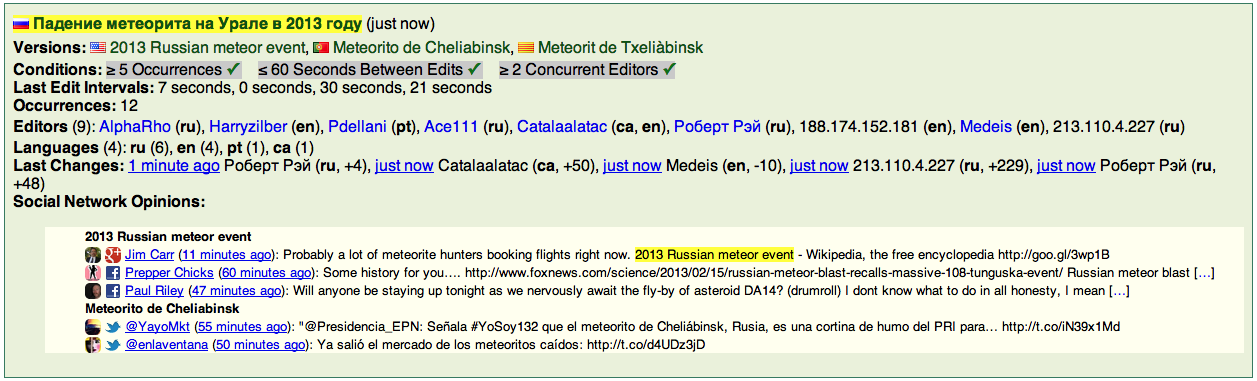
\includegraphics[width=\linewidth]{wikipedia-live-monitor.png}
  \caption[Screenshot with an article cluster of four concurrently edited articles]
    {Screenshot with an article cluster of four concurrently edited articles
    (ru, en, pt, ca). All breaking news criteria are fulfilled,
    the cluster is a~breaking news candidate.
    Cross-language social network search results for en and pt can be seen.}
  \label{fig:screenshotwikilivemon}
\end{figure*}

\section{Implementation Details}

\subsection{Wikipedia Recent Changes}
\label{sec:wikipedia-recent-changes}

As described earlier, our application monitors concurrent edit spikes
on different language versions of Wikipedia.
In the current implementation, we monitor \emph{all}
285 different Wikipedias, 8 with
$\geq$~1,000,000 and 38 with $\geq$~100,000 articles%
\footnote{\url{http://meta.wikimedia.org/wiki/List_of_Wikipedias},
accessed July 15, 2013}
including a~long-tail of smaller Wikipedias.
Changes to any single one article are communicated by a~chat bot
over Wikipedia's own Internet Relay Chat~(IRC) server (\url{irc.wikimedia.org}),%
\footnote{\url{http://meta.wikimedia.org/wiki/IRC/Channels\#Raw_feeds}, accessed July 15, 2013}
so that parties interested in the data can listen to the changes as they happen.
For each language version, there is a~specific chat room following the pattern
\texttt{"\#" + language + ".wikipedia"}.
For example, changes to Russian Wikipedia articles will be streamed to the room
\texttt{\#ru.wikipedia}.
A~special case is the room \texttt{\#wikidata.wikipedia} for Wikidata~%
~\cite{vrandecic2012wikidata},
a~platform for the collaborative acquisition and maintenance
of structured data to be used by
Wikimedia projects like Wikipedia.
A~sample chat message with the components separated
by the asterisk character \texttt{`*'}
announcing a~change can be seen in the following.
\texttt{"[[Juniata River]]
http://en.wikipedia.org/w/index.php?diff=\-516269072\&oldid=514-659029 *
Johanna-Hypatia * (+67)
Category:Place names of Native American origin in Pennsylvania"}.
The message components are (i)~article name, (ii)~revision URL,
(iii)~Wikipedia editor handle, and (iv)~change size and change description.

\subsection{Article Clusters}

We cluster edits of articles about the same topic,
but written in different languages, in article clusters.
The example of the English
\texttt{en:2013\_Russian\_meteor\_event}
and the corresponding Russian article
\texttt{ru:{\fontencoding{T2A}\selectfont Падение\_метеорита\_на\_Урале\_в\_2013\_году}}
that are both in the same cluster illustrate this.
We use the Wikipedia API to retrieve language links for a~given article.
The URL pattern for the API is as follows.
\texttt{http://\$LANGUAGE.\-wikipedia.org/w/api.php?action=query\&prop=langlinks\&titles=\$ARTICLE\&form\-at=json}. We work with the JSON representation.

\subsection{Comparing Article Revisions}
\label{sec:comparing-article-revisions}

The Wikipedia API provides means to retrieve the actual changes
that were made during an edit including additions, deletions,
and modifications in a~\texttt{diff}-like manner.
The URL pattern is as follows.
\texttt{http://\$LANGUAGE.wikipedia.org/w/api.php?action=co\-mpare\&torev=\$TO\&fromrev=\$FROM\&format=json}.
This allows us to classify edits in categories like, \emph{e.g.},
negligible trivial edits (punctuation correction) and
major important edits (new paragraph for an article),
which helps us to disregard seemingly concurrent edits
in order to avoid false-positive alerts.

\subsection{Breaking News Criteria}

Our application \emph{Wikipedia Live Monitor} puts
detected article clusters in a~monitoring loop in which they remain
until their time-to-live (240~seconds) is over.
In order for an article cluster in the monitoring loop
to be identified as breaking news candidate,
the following breaking news criteria have to be fulfilled.

\begin{description}
  \itemsep0em
  \item[$\geq$~5~Occurrences:] An article cluster must have occurred
  in at least 5~edits.
  \item[$\leq$~60~Seconds Between Edits:] An article cluster may have
  at maximum 60~seconds in between edits.
  \item[$\geq$~2~Concurrent Editors:] An article cluster must have been edited
  by at least 2~concurrent editors.
  \item[$\leq$~240~Seconds Since Last Edit:] An article cluster's last edit
  may not be longer ago than 240~seconds.
\end{description}

The exact parameters of the breaking news criteria above
were \emph{determined empirically} by analyzing Wikipedia edits
over several hours and repeatedly adjusting the settings until
major news events happening at the same time were detected.
The resulting dataset split into three chunks has been made publicly available.%
\footnote{\url{https://www.dropbox.com/sh/2qsg1zhb8p35fxf/Dghn55y0kh},
accessed July 15, 2013}

\subsection{Social Network Plausibility Checks}

When a~breaking news candidate has been identified,
we use cross-language full-text social network searches
on the social networks Twitter, Facebook, and \googleplus
as a~plausibility check.
As the \emph{article titles} of all language versions
of the particular article's cluster are know,
we use these very article titles as search queries for cross-language searches,
as can be seen in \autoref{fig:screenshotwikilivemon}.
This approach greatly improves the recall of the social network search,
however, requires either machine translation or an at least basic understanding
of the languages being searched in.
Currently the plausibility checking step is not yet fully automated,
as the search results are for the time being meant to be consumed by \emph{human evaluators}.
Driven by (H1), we assume breaking news events are being discussed on social networks.
We will show arguments for this assumption in \autoref{sec:premature-evaluation}.
For now, we expect social networks to be a~short period ahead of Wikipedia.
In consequence, if the human rater can find positive evidence
for a~connection between social network activities and Wikipedia edit actions,
the breaking news candidate is confirmed to indeed represent breaking news.

\subsection{Application Pseudocode}

The \emph{Wikipedia Live Monitor} application has been implemented in Node.js,
a~server side JavaScript software system
designed for writing scalable Internet applications.
Programs are created using event-driven, asynchronous input/output operations
to minimize overhead and maximize scalability.
\autoref{code:pseudocode-wikipedia-monitor} shows the pseudocode of the two main event loops of the
\emph{Wikipedia Live Monitor} application.
The actual implementation is based on
Martyn Smith's Node.js IRC library%
\footnote{\url{https://github.com/martynsmith/node-irc},
accessed July 15, 2013} and
the WebSockets API and protocol~\cite{hickson2012websockets},
wrapped by  Guillermo Rauch's library Socket.IO.%
\footnote{\url{http://socket.io/},
accessed July 15, 2013}


\begin{lstlisting}[caption=Two main event loops
  of the application,
  label=code:pseudocode-wikipedia-monitor, escapechar=§]
§\textbf{Input: irc, listening on Wikipedia recent changes}§
§\textbf{Output: breakingNewsCandidates, breaking news candidates}§

monitoringLoop = articleClusters = breakingNewsCandidates = {}

§\textit{\# Event loop 1:}§
§\textit{\# When a new message arrives}§
irc.on.message §\textbf{do (article)}§
  langRefs = getLanguageReferences(article)
  articleRevs = getArticleRevisions(article)
  cluster = clusterArticles(article, langRefs)

  §\textit{\# Create new cluster for previously unseen article}§
  §\textbf{if}§ cluster not in monitoringLoop
    monitoringLoop.push(cluster)
    articleClusters.push(cluster)
    updateStatistics(cluster)
    emit.newCluster(cluster, articleRevs)
  §\textit{\# Update existing cluster, as the article was seen before}§
  §\textbf{else}§
    updateStatistics(cluster)
    emit.existingCluster(cluster, articleRevs)
    §\textit{\# Check breaking news criteria}§
    §\textbf{if}§ cluster.occurrences >= 5
      §\textbf{if}§ cluster.secsBetweenEdits <= 60
        §\textbf{if}§ cluster.numEditors >= 2
          §\textbf{if}§ cluster.secsSinceLastEdit <= 240
            socialNetworks.search(langRefs)
            breakingNewsCandidates.push(cluster)
            emit.breakingNewsCandidate(cluster)
          §\textbf{end if}§
        §\textbf{end if}§
      §\textbf{end if}§
    §\textbf{end if}§
  §\textbf{end if}§
  §\textbf{return}§ breakingNewsCandidates
§\textbf{end do}§

§\textit{\# Event loop 2:}§
§\textit{\# Remove too old clusters regularly}§
timeout.every.240seconds §\textbf{do}§
  §\textbf{for each}§ cluster §\textbf{in}§ monitoringLoop
    §\textbf{if}§ cluster.secsSinceLastEdit >= 240
      monitoringLoop.remove(cluster)
      articleClusters.remove(cluster)
    §\textbf{end if}§
  §\textbf{end for}§
§\textbf{end do}§
\end{lstlisting}

\section{Evaluation}
\label{sec:premature-evaluation}

In \autoref{sec:hypotheses-and-research-questions},
we have set up three hypotheses.
(H1) has been proven by Hu \emph{et~al.}\ in~\cite{hu2012breakingnews} for Twitter.
We argue that it can be generalized to other social networks
and invite the reader to have a~look at our dataset,
where the lively discussions about breaking news candidates
on the considered social networks Twitter, Facebook, and \googleplus
support the argument.
It is hard to prove (H2), as the concept of \emph{important breaking news}
is vague and dependent on one's personal background, however,
all evidence suggests that (H2) indeed holds true,
as, to the best of our knowledge and given our background,
what the authors consider \emph{important breaking news}
is represented on at least one language version of Wikipedia.
(H3) has been examined by Osborne \emph{et~al.}\ in~\cite{osborne2012bieber}.
In the paper, they suggest that Wikipedia lags about two hours behind Twitter.
It has to be noted that they look at hourly accumulated page (article) \emph{view} logs,
where we look at realtime article \emph{edit} log streams.
Our experiments suggest that the lag time of two hours
proposed by Osborne \emph{et~al.}\ may be too conservative.
A~conservative estimation at this stage is that the lag time
for breaking news is more in the range of 30 minutes,
and for global breaking news like celebrity deaths
in the range of five minutes and less,
albeit the edits by our experience will be small and iterative
(\emph{e.g.}, ``X is a'' to ``X was a,'' or the addition of a~death date),
followed by more consistent thorough edits.

The (at time of writing) recent breaking news event
of the resignation of \emph{Pope Benedict~XVI} helps respond to (Q1).
The three first edit times of the Pope's English Wikipedia article%
\footnote{\url{http://en.wikipedia.org/w/index.php?title=Pope_Benedict_XVI&action=history},
accessed July 15, 2013}
after the news broke on February 11, 2013 are as follows
(all times in UTC): 10:58, 10:59, 11:02.
The edit times of the French article%
\footnote{\url{http://fr.wikipedia.org/w/index.php?title=Beno\%C3\%AEt_XVI&action=history}, accessed July 15, 2013}
are as follows: 11:00, 11:00, 11:01.
This implies that by looking at only two language versions of Wikipedia
(the actual number of monitored versions is 285) of the Pope article,
the system would have reported the news at 11:01.
The official Twitter account of Reuters announced%
\footnote{\url{https://twitter.com/Reuters/status/300922108811284480},
accessed July 15, 2013} the news at 10:59.
Vatican Radio's announcement%
\footnote{\url{http://de.radiovaticana.va/Articolo.asp?c=663810},
accessed July 15, 2013} was made at 10:57:47.

Not all breaking news events have the same global impact as the Pope's resignation,
however, the proposed system was shown to work very reliably
also for smaller events of more regional impact, for example,
when \emph{Indian singer Varsha Bhosle} committed suicide%
\footnote{\url{http://en.wikipedia.org/wiki/Varsha_Bhosle},
accessed July 15, 2013} on October 8, 2012.
A~systematic evaluation of (Q1)~compulsorily can only be done by random samples,
which has turned out positive results so far.
Again, we invite the reader to explore our dataset and to conduct own experiments.
A~systematic evaluation of (Q2) requires a~commonly shared dataset,
which we have provided, however, at this point in time, we do not have access to the system
of Osborne \emph{et~al.}

Regarding \emph{Wikipedia Live Monitor}'s scalability,
we already scale the monitoring system
up to currently \emph{all} 285~Wikipedias on a~standard consumer laptop
(mid-2010 MacBook Pro, 2.66~GHz Intel Core~2, 8~GB RAM),
which proves the efficiency of the Node.js architecture
for this kind of event-driven applications.
In practice, the majority of the smaller Wikipedias
being very rarely updated,
we note that limiting ourselves to the Wikipedias
with $\geq$~100,000 articles results in no remarkable loss of recall.

\section{Future Work}

Future work will mainly address two areas.
First, the \emph{automated categorization of edits on Wikipedia}
needs to be more fine-grained.
In the context of breaking news detection, not all edits are equally useful.
An image being added to an article is an example of an edit
that usually will not be important.
In contrast, the category ``Living people'' being removed from an article
is a~strong indicator of breaking (sad) news.
Second, the \emph{connection between social network search and Wikipedia edits}
needs to be made clearer.
In an initial step, the concrete changes to an article, as detailed in
\autoref{sec:comparing-article-revisions}, can be compared with
social network microposts using a~cosine similarity measure.
More advanced steps can exploit the potential knowledge from Wikipedia edits
(\emph{e.g.}, category ``Living people'' removed implies a~fatality).

\section{Conclusions}

In this chapter, we have shown an application called \emph{Wikipedia Live Monitor}
and released its source code under the Apache~2.0 license.
This application monitors article edits on 285 different language versions of Wikipedia.
It detects breaking news candidates according to well-defined breaking news criteria,
whose exact parameters were determined empirically
and the corresponding dataset made available publicly.
We have shown how cross-language full-text social network searches are used
as plausibility checks to avoid false-positive alerts.
Concluding, our approach has revealed very promising results
and actionable next steps in future work
for improving the application.

\section*{Chapter Notes}
This chapter is partly based on the following publications.

\begin{itemize}
  \interlinepenalty10000
  \item \onlyfullcite{steiner2013mj}.
  \item \onlyfullcite{steiner2011crowdsourcingevent}.
\end{itemize}

\clearpage
\printbibliography[heading=subbibliography]
\chapter{Media Item Extraction}
\label{cha:media-item-extraction}

% the code below specifies where the figures are stored
\ifpdf
    \graphicspath{{6_media_item_extraction/figures/PNG/}{6_media_item_extraction/figures/PDF/}{6_media_item_extraction/figures/}}
\else
    \graphicspath{{6_media_item_extraction/figures/EPS/}{6_media_item_extraction/figures/}}
\fi

\section{Introduction}

Before the rise of social networks,
event coverage was mostly an affair of professional news agencies.
The widespread availability of mobile phones
with higher resolution cameras has transformed
citizens into witnesses who are used to comment
and share media illustrating events on social networks.
Some examples with global impact
include the shootings in
Ut{\o}ya,\footnote{\url{http://en.wikipedia.org/wiki/2011_Norway_attacks},
accessed July 15, 2013}
which first appeared on Twitter,
the capture and arrest of Muammar
Gaddafi,\footnote{\url{http://en.wikipedia.org/wiki/Death_of_Muammar_Gaddafi},
accessed July 15, 2013}
which first appeared on YouTube,
or the emergency ditching of a~plane in the Hudson
river,\footnote{\url{http://en.wikipedia.org/wiki/US_Airways_Flight_1549},
accessed July 15, 2013}
which first appeared on Twitpic.
Some news
communities\footnote{\url{http://www.citizenside.com/},
accessed July 15, 2013}
have even specialized in aggregating and brokering
such user-generated content.
Events, such as sports matches or concerts are
largely illustrated by social media,
albeit distributed over many social networks.

In this chapter, we tackle the challenge of reconciling
social media data that illustrates known events,
but that is spread over various social networks,
all with the objective of creating visual event summaries.
We propose a~social-network-agnostic
approach for the extraction of photos and videos covering events.
We want to emphasize that in this chapter we do \emph{not}
put the focus on event detection (we have done that in \autoref{cha:eventdetection}).
The events we are dealing with in this chapter
were known beforehand and we use specific
human-chosen search terms to find illustrating media.

We first recall the definitions previously made in
\autoref{sec:definition} and add formal definitions
of the terms \emph{event},
\emph{media item extraction},
\emph{Application Programming Interface},
and \emph{Web scraping}.

\begin{description}
  \item[Social Network:]
       A~social network is an online service or media platform
       that focuses on building and reflecting
       relationships among people
       who share common interests and/or activities.
  \item[Media Item:]
       A~media item is defined as
       a~photo\footnote{We choose the term \emph{photo}
       over the term \emph{image} as
       Facebook, Twitter, and \googleplus use it.}
       or video file that is publicly shared or published
       on at least one social network.
  \item[Micropost:]
       A~micropost is defined as a~textual status message
       on a~social network
       that can optionally be accompanied by a~media item.
  \item[Event:]
       An event is defined as a~phenomenon that has happened
       or that is scheduled to happen.
       It is an observable occurrence grouping persons,
       places, times, and activities while being often
       documented by people through different media~%
       \cite{liu2011events}.
  \item[Media Item Extraction:]
       The process of leveraging search functionalities of
       social networks to find references to media items,
       which allows for storing those media items in binary form.
  \item[Application Programming Interface (API):]
       An API is a~programmatic specification intended to be used
       as an interface by software components on client and server
       to communicate with each other.
  \item[Web scraping]
       The term Web scraping means the process of
       automatedly extracting information from Web pages.
       Web scraping involves practical solutions based on
       existing technologies that are often entirely \emph{ad hoc}.
       Examples of such technologies are regular expressions,
       Document Object Model (DOM)
       parsing~\cite{lehors2004dom},
       or CSS selectors~\cite{hunt2012cssselectors}.
       The difference between \emph{Web scraping}
       and the related concept of \emph{screen scraping}
       is that screen scraping relies on the visual layout of a~Web page,
       while Web scraping relies on the textual
       and/or hierarchical structure.
\end{description}

\section{Related Work}

Related work covers research
that aims to collect, align, and organize media
for trends or events.
Liu \emph{et~al.}\ combine semantic inferencing and visual analysis
to automatically find media to illustrate
events~\cite{liu2011events}.
They interlink large datasets of event metadata
and media with the Linking Open Data
Cloud~\cite{bizer2011statelodcloud,cyganiak2011lodcloud}.
In~\cite{liu2011socialmedia}, they show how visual summaries
of past events providing viewers with a~more compelling feeling
of the event's atmosphere can be created
based on a~method to automatically detect and identify events
from social media sharing websites.
Approaches to alignment use visual, temporal,
and spacial similarity measures to map multiple photo streams of
the same events~\cite{yang2011photostream}.
Other ways to collect and order media from social networks use
media-driven metadata such as geospatial
information~\cite{crandall2009mappingphotos}.
Becker \emph{et~al.}\ show in~\cite{becker2010eventidentification}
how to exploit the rich context associated with social media
content, including user-provided annotations
and automatically generated information.
Using this rich context, they define similarity metrics
to enable online clustering of media to events.
In~\cite{becker2012plannedevents}, the same authors develop
recall-oriented query formulation strategies
based on noisy event metadata
from event aggregation platforms.

\section{Social Networks and Media Items}                                    \label{sec:social-networks}

Most social networks offer a~search functionality that allows for
content to be retrieved based on search terms,
with or without more advanced search operators
such as exclusion, inclusion, phrase search, \emph{etc.}
Each social network has special constraints
regarding the supported search operators or filtering options.

Social networks are often perceived as
\emph{walled gardens}~\cite{simonds2008walledgarden}
due to the full control of the network operator
over content and media on the social network in question,
oftentimes accessible exclusively by social network members.
This network lock-in effect was excellently illustrated
by David Simonds in a~cartoon that first appeared
in the English-language weekly news and
international affairs publication \emph{The Economist},
reproduced in \autoref{fig:walled-gardens}.
While some social networks (\emph{e.g.}, Twitter)
have full read and write access via specified APIs,
other social networks (\emph{e.g.}, \googleplus)
currently only have read API access.
In some cases, however, API access is limited,
so that not all desired pieces of information is exposed
(\emph{e.g.}, view counts with Img.ly),
which forces people interested in that data
to fall back to Web scraping.
It is to be noted that if the directives in the
\texttt{robots.txt} file are respected,
Web scraping \emph{per~se} is not an illegal practice,
as only public information is being accessed,
comparable to the level of access that common Web search engines have.
The Robot Exclusion Standard,
also referred to as \texttt{robots.txt} protocol,
is a~widely respected convention to prevent cooperating Web crawlers
and other Web robots
from accessing all or part of a~website
that is otherwise publicly viewable.

\begin{figure}[!ht]
  \centering
  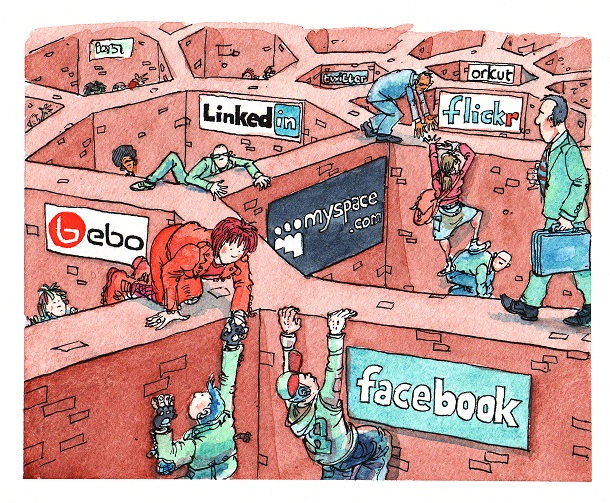
\includegraphics[width=0.7\linewidth,
    trim=16px 17px 12px 15px,clip]{davidsimonds.jpg}
  \caption[Social networks as walled
    gardens illustrated by David Simonds]
    {Social networks as walled gardens illustrated by David Simonds}
  \label{fig:walled-gardens}
\end{figure}

\section{Media Extractor}
\label{sec:media-extractor}

In this section, we first introduce a~common data format
that we have developed as an abstraction layer on top of the native
data formats used by the considered social networks.
We then explain the architecture
of different kinds of media item extractors.
Finally, we describe the processing steps
that we apply to each extracted media item.

\subsection{Abstraction Layer Data Format}
\label{sec:data-format}

Each social network uses a~different data representation schema.
While all social networks with API access are
JSON-based~\cite{crockford2006json}, the differences in both
supported social network features and media item support level,
as was outlined in detail in
\autoref{sec:description-of-popular-social-networks} and
\autoref{sec:classification-of-social-networks},
are also reflected in the returned JSON data.
We therefore propose a~common abstraction layer
on top of the native data formats of all considered social networks.
It is in the nature of any abstraction
that it can only represent the
greatest common divisor of all social networks.
We show the abstraction layer in the following
with the help of a~concrete example,
stemming from a~query to the media extractor
that will be explained in more detail
in the upcoming \autoref{sec:media-item-extractors}.
The media extractor was used to query for media items
that match the search term \emph{hamburg}.
\autoref{code:facebook} shows sample output of the media extractor
for a~Facebook post, which was processed
with named entity extraction and disambiguation
as was detailed in \autoref{cha:micropost-annotation}.

\begin{description}
  \itemsep0em
  \item[\texttt{mediaUrl}] Deep link to a~media item
  \item[\texttt{posterUrl}] Deep link to a~thumbnail for photos
    or still frame for videos
  \item[\texttt{micropostUrl}] Deep link to the micropost on
    the social network
  \item[\texttt{micropost}] Container for a~micropost
  \begin{description}
    \item[\texttt{html}] Text of the micropost,
      possibly with HTML markup
    \item[\texttt{plainText}] Text of the micropost with
      potential HTML markup removed
    \item[\texttt{entities}] Extracted and disambiguated
      named entities from the micropost text
  \end{description}
  \item[\texttt{userProfileUrl}] Deep link to the user's
    profile on the social network
  \item[\texttt{type}] Type of the media item,
    can be \texttt{photo} or \texttt{video}
  \item[\texttt{timestamp}] Number of milliseconds between
    1 January 1970 00:00:00 UTC and the moment
    when the micropost was published
  \item[\texttt{publicationDate}] Date in ISO 8601
    format (YYYY-MM-DDTHH:MM:SSZ) when the micropost was published
  \item[\texttt{socialInteractions}] Container for social
    interactions
  \begin{description}
  \item[\texttt{likes}] Number of times a~micropost was liked, or
    \texttt{unknown}
  \item[\texttt{shares}] Number of times a~micropost was shared, or
    \texttt{unknown}
  \item[\texttt{comments}] Number of comments a~micropost
    received, or \texttt{unknown}
  \item[\texttt{views}] Number of views a~micropost reached, or
    \texttt{unknown}
  \end{description}
\end{description}

\begin{lstlisting}[caption={[Sample output of the media extractor]{Sample output of the media extractor
  showing a~Facebook post processed with named entity extraction
  and disambiguation (slightly shortened for legibility)}},
  label={code:facebook}]
{
  "mediaUrl": "http://video.ak.fbcdn.net/...",
  "posterUrl": "http://external.ak.fbcdn.net/...",
  "micropostUrl": "https://www.facebook.com/permalink.php?story_fbid=
    231781590231029&id=1254772464",
  "micropost": {
    "html": "Videoed between Hamburg and Snyder. Thought I would share.",
    "plainText": "Videoed between Hamburg and Snyder. Thought I would share.",
    "entities": [
      [
        {
          "name": "Hamburg",
          "relevance": 0.82274,
          "uri": "http://dbpedia.org/resource/Hamburg"
        },
        {
          "name": "Snyder",
          "relevance": 0.857,
          "uri": "http://dbpedia.org/resource/Snyder,_Texas"
        }
      ]
    ]
  },
  "userProfileUrl": "https://www.facebook.com/profile.php?id=1254772464",
  "type": "video",
  "timestamp": 1326371479000,
  "publicationDate": "2012-01-12T12:31:19Z",
  "socialInteractions": {
    "likes": 0,
    "shares": 0,
    "comments": 3,
    "views": null
  }
}
\end{lstlisting}

\subsection{Media Item Extractors}
\label{sec:media-item-extractors}

We have developed a~combined media extractor composed of
separate media item extractors for the seven social networks
\googleplus, Myspace, Facebook, Twitter, Instagram, YouTube,
and Flickr, with additional support for the media sharing
platforms Img.ly, Imgur, Lockerz,\footnote{Dysfunctional since April 2013 when the service shut down its API access} Yfrog, MobyPicture, and Twitpic.
The media extractor takes as input a~search term that is relevant
to a~known event, \emph{e.g.}, the term \emph{boston celtics}
for a~recent match of the Basketball team Boston Celtics.
This search term gets forwarded to the search APIs
of all social networks in parallel.
Each social network has a~30 seconds timeout window
to deliver its results.
When the timeout is reached
or when all social networks have responded,
the available results are aligned according to the data format
defined in \autoref{sec:data-format}.
Media items and the relevant metadata like view count, comments,
\emph{etc.}\ are retrieved either directly or via Web scraping.
For some social networks, \emph{e.g.}, Img.ly,
a~combination of Web scraping and API access is required
since the API does not return all necessary fields
of our data format.
While we could default to Web scraping
to obtain all relevant data,
it is more robust to use API access wherever possible
and only fall back to the more brittle Web scraping
for the parts not covered by API access.

\paragraph{Special Role of Twitter:}

Twitter (\autoref{sec:twitter})
plays a~special role, as it can be used as
a third-order support social network,
as was detailed previously in \autoref{sec:classification-of-social-networks}.
This means that the micropost text is located on Twitter,
but the referenced media items are located
on third-party media platforms.
Due to the length limitation for tweets of 140 characters,
short URLs are used on the service.
We search for the search term in question (\emph{e.g.},
following up from the example before, \emph{boston celtics}),
but combine it with the short URL domain parts of
the media platforms.
For example, the short domain URL of the social network Flickr
(\autoref{sec:flickr})
is \url{flic.kr}, where the long domain URL is \url{flicker.com}.
The short domain URL of Instagram
(\autoref{sec:instagram}) is \url{instagr.am},
where the long domain URL is \url{instagram.com}, \emph{etc.}
We have created a~list of all known short domain URLs for the
considered media platforms so that the complete search query
for Twitter is the actual search term,
combined with this list of short domain URLs:

\emph{boston celtics AND (flic.kr OR instagr.am OR ...)}

\noindent The complete data flow is illustrated in the
architectural diagram in \autoref{fig:architecture}.
As a~side note, Twitter on its website now has its own
media extractor based on Twitter Cards~\cite{wang2012twitter}
with support for some of of the media platforms,
however, our own media extractor goes beyond Twitter's offer,
especially since Facebook-owned Instagram's latest break-up with
Twitter.\footnote{\url{http://techcrunch.com/2012/12/05/kevin-systrom-on}, accessed July 15, 2013}

\begin{figure}
  \centering
  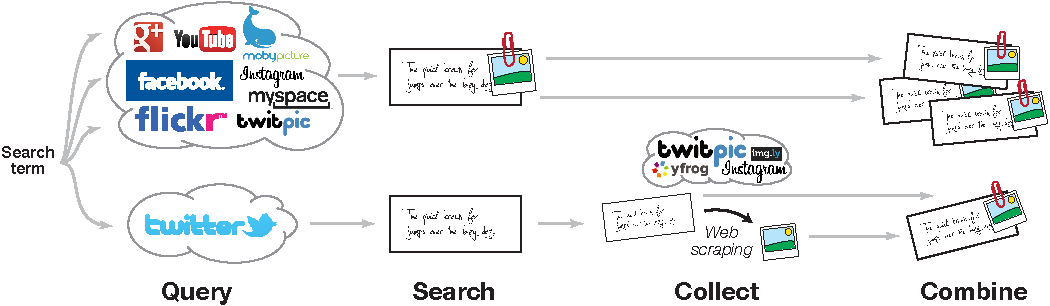
\includegraphics[width=1.0\linewidth]{architecture.pdf}
  \caption[Overview of the media extractor]
    {Overview of the media extractor:
    hybrid approach to the media item extraction task using
    a~combination of API access and Web scraping}
  \label{fig:architecture}
\end{figure}

\section{Evaluation}

We have run experiments in the time period of January 10 to 19, 2012,
during which we have randomly selected nine events
that received broad social media coverage.
For these events, we have collected media items and microposts
using our media extractor.
In the following, we will provide a~short summary of the nine selected events
in order to give the reader the necessary background knowledge.

\begin{description}
  \item[Assad Speech]
       On January 10, 2012, Syrian President Bashar al-Assad
       delivered a~televised talk defending his
       government's actions and motivations, despite world
       pressure on his government for its 10-month
       crackdown on
       protesters.
       Activists say the operation has led to nearly
       6,000 or more estimated deaths.\footnote{\url{http://www.cnn.com/2012/01/10/world/meast/syria-unrest/},
       accessed July 15, 2013}
  \item[CES Las Vegas]
       The International Consumer Electronics Show (CES) is
       a~major technology-related trade show held each January
       in the Las Vegas Convention Center. Not open to the public,
       the Consumer Electronics Association-sponsored show
       typically hosts previews of products and new product
       announcements.
       CES Las Vegas took place from January 11 to 13,
       2012.\footnote{\url{http://www.cesweb.org/},
       accessed July 15, 2013}\\
       \textbf{Cut the Rope Launch:}
       On January 10, 2012 during Steve Ballmer's final keynote
       at the International Consumer Electronics Show, the
       HTML5 version of the popular mobile game \textit{Cut the
       Rope} was announced. This is a~sub-event of CES Las
       Vegas.\footnote{\url{http://ces.cnet.com/8301-33377_1-57356403/},
       accessed July 15, 2013}\\
       \textbf{Ubuntu TV Launch:}
       Ubuntu TV by Canonical, based on the user interface Unity,
       is a~variant of the Ubuntu operating system, designed to be
       a~Linux distribution specially adapted for embedded systems
       in televisions. It was announced by Canonical on January
       10, 2012, at
       CES.\footnote{\url{http://www.theverge.com/2012/1/9/2695387/ubuntu-tv-video-hands-on},
       accessed July 15, 2013}
  \item[Costa Concordia Disaster]
       The Costa Concordia is an Italian cruise ship that hit
       a~reef and partially sank on January 13, 2012 off the
       Italian coast. The vessel ran aground at Isola del Giglio,
       Tuscany, resulting in the evacuation of 4,211
       people.\footnote{\url{http://en.wikipedia.org/wiki/Costa_Concordia_disaster},
       accessed July 15, 2013}
  \item[Dixville Notch]
       Dixville Notch is an unincorporated village in Dixville
       township of Coos County, New Hampshire, USA, best known in
       connection with its longstanding middle-of-the-night vote in
       the U.S. presidential election. In a~tradition that started
       in the 1960 election, all the eligible voters in Dixville
       Notch gather at midnight in the ballroom of The Balsams.
       This year, on January 10, 2012, the voters cast their
       ballots and the polls officially closed one minute
       later.\footnote{\url{http://www.washingtonpost.com/2012/01/09/gIQANslKnP_story.html},
       accessed July 15, 2013}
  \item[Free Mobile Launch]
       Free Mobile is a~French mobile broadband company, part of
       the Iliad group. On January 10, 2012, a~long-awaited mobile
       phone package for \EUR{19.99} with calls included to 40
       countries, texts, multimedia messages and Internet was
       announced by the Iliad group's Chief Strategy Officer
       Xavier
       Niel.\footnote{\url{http://www.nytimes.com/2012/01/11/technology/iliad-takes-aim-at-top-mobile-operators-in-france.html},
       accessed July 15, 2013}
  \item[Blackout SOPA]
       The Stop Online Piracy Act (SOPA) is a~bill of the United
       States proposed in 2011 to fight online trafficking in
       copyrighted intellectual property and counterfeit goods.
       On January 18, the English Wikipedia, and several
       other Internet companies coordinated a~service blackout
       to protest SOPA and its sister bill, the Protect IP Act
       (PIPA).
       Other companies, including Google, posted links and
       photos in an effort to raise
       awareness.\footnote{\url{http://sopablackout.org/learnmore/},
       accessed July 15, 2013}
  \item[Christian Wulff Case]
       Since December 2011, former German President Christian
       Wulff faces controversy over discrepancies in statements
       about a~loan while being governor of Lower Saxony.
       It was revealed that he had applied pressure
       on Springer Press to delay revelations on the issue until
       he was back from a~visit abroad. When Wulff found out that
       a~tabloid was going to break the story, he left a~message
       on their voice mail in which he threatened to take legal
       action.\footnote{\url{http://www.spiegel.de/international/germany/0,1518,804631,00.html},
       accessed July 15, 2013}
\end{description}

\subsection{Dataset}
Our data set contained 448 photos with an average file size of
$\sim$0.7MB and 143 videos.
Some videos are no longer available due to either
account termination or video takedown by the user
(Assad, Dixville).
\autoref{tab:number-media} shows the total
numbers of retrieved photos and videos of the media extractor.
Table cell values marked with $n+$ signify that there were more
results, but that only $n$ results were considered.
We have calculated the precisions for each event for both video
and photo separately; the overall photo precision was $0.73$,
and the overall video precision was $0.54$.
We note that these values were calculated \emph{before}
any pruning step, \emph{i.e.}, before taking into account
the additional textual information from microposts like
potential extracted named entities.
The dataset is very diverse with respect to photo quality,
photo format, and naturally, content.
It ranges from entirely sharp screenshots
in all sorts of formats (\emph{e.g.},
screenshots of the Google homepage for the Blackout SOPA event
to screenshots of a~wide banner advertisement),
over to blurry cell phone photos in standard photo formats
(\emph{e.g.}, photos of the stage
for the Free Mobile Launch event).
\autoref{fig:sequences} shows sample photos for
some of the considered nine events.
We have observed that more than one search session
with different combinations of search terms~%
\cite{becker2010eventidentification,becker2012plannedevents}
is necessary in order to obtain a~satisfactory recall.
Query strategies developed by Becker~\cite{becker2012plannedevents}
that combine different combinations of event title,
event venue, and event city work consistently well.

\begin{sidewaystable}[!ht]
  \centering
  \footnotesize
  \begin{tabular}{|l|c|c|c|c|c|c|c|c|c|c|c|c|c|c|c|c|c|c|}
    \hline
    \multicolumn{1}{|c|}{\textbf{Social}} & \multicolumn{2}{c|}{\textbf{Assad}} & \multicolumn{2}{c|}{\textbf{CES}} &
    \multicolumn{2}{c|}{\textbf{Concordia}} & \multicolumn{2}{c|}{\textbf{Dixville}} & \multicolumn{2}{c|}{\textbf{Free}} &
    \multicolumn{2}{c|}{\textbf{Ropes}} & \multicolumn{2}{c|}{\textbf{SOPA}} & \multicolumn{2}{c|}{\textbf{Ubuntu}} &
    \multicolumn{2}{c|}{\textbf{Wulff}} \\
    \cline{2-19}
    \multicolumn{1}{|c|}{\textbf{Network}} & \textbf{P} & \textbf{V} & \textbf{P} & \textbf{V} & \textbf{P} & \textbf{V} &
    \textbf{P} & \textbf{V} & \textbf{P} & \textbf{V} & \textbf{P} & \textbf{V} & \textbf{P} & \textbf{V} & \textbf{P} &
    \textbf{V} & \textbf{P} & \textbf{V} \\
    \hline
    \textbf{\googleplus} & 3 & 2 & 5 & 3 & 15 & 1 & 4 & 1 & 6 & 0 & 5 & 1 & 5 & 0 & 6 & 1 & 7 & 0\\
    \textbf{Myspace} & 0 & 0 & 0 & 0 & 10+ & 0 & 9 & 0 & 1 & 0 & 6 & 0 & 0 & 0 & 0 & 0 & 8 & 0\\
    \textbf{Facebook} & 0 & 0 & 0 & 1 & 0 & 1 & 0 & 0 & 0 & 0 & 0 & 0 & 0 & 2 & 0 & 0 & 0 & 0\\
    \textbf{Twitter} & 2 & 0 & 2 & 0 & 3 & 0 & 3 & 0 & 2 & 0 & 4 & 0 & 5 & 0 & 0 & 0 & 2 & 0\\
    \textbf{Instagram} & 0 & 0 & 20+ & 0 & 20+ & 0 & 0 & 0 & 20+ & 0 & 20+ & 0 & 20+ & 0 & 0 & 0 & 2 & 0\\
    \textbf{YouTube} & 0 & 10+ & 0 & 10+ & 0 & 10+ & 0 & 3 & 0 & 10+ & 0 & 10+ & 0 & 10+ & 0 & 10+ & 0 & 10+\\
    \textbf{Flickr} & 10+ & 0 & 10+ & 6 & 10+ & 10+ & 10+ & 10+ & 10+ & 0 & 10+ & 10+ & 10+ & 0 & 10+ & 9 & 10+ & 2\\
    \textbf{MobyPic} & 0 & 0 & 1 & 0 & 4 & 0 & 0 & 0 & 2 & 0 & 20+ & 0 & 1 & 0 & 2 & 0 & 3 & 0\\
    \textbf{Twitpic} & 0 & 0 & 20+ & 0 & 18 & 0 & 1 & 0 & 20+ & 0 & 20+ & 0 & 19 & 0 & 2 & 0 & 20+ & 0\\
    \hline
    \textbf{Total} & 15 & 12 & 58 & 20 & 80 & 22 & 27 & 14 & 61 & 10 & 85 & 21 & 60 & 12 & 20 & 20 & 52 & 12\\
    \hline
    \textbf{Relevant} & 12 & 7 & 39 & 18 & 61 & 15 & 8 & 2 & 46 & 4 & 76 & 14 & 43 & 5 & 18 & 13 & 39 & 7\\
    \hline
    \hline
    \textbf{Precision} & .80 & .58 & .67 & .90 & .76 & .55 & .30 & .14 & .75 & .40 & .89 & .67 & .71 & .42 & .90 & .65 & .75 & .58\\
    \hline
  \end{tabular}
  \caption[Number of photos and videos collected for nine events]{Number of photos and videos collected for nine events happening between January 10--19, 2012 grouped by social networks, separated in photo (P) and video (V) results. Overall \textbf{photo precision: 0.73}. Overall \textbf{video precision: 0.54}. Note that this is before post-processing.}
  \label{tab:number-media}
\end{sidewaystable}

\begin{figure*}
\begin{tabular}{p{\textwidth}}
\eventtitle{Blackout SOPA}
\begin{thumbsequence}
    
\includegraphics[height=\thumbheight]{sopa/looseduplicate1.jpg}
    
\includegraphics[height=\thumbheight]{sopa/looseduplicate2.jpg}
    
\includegraphics[height=\thumbheight]{sopa/looseduplicate3.jpg}
    
\includegraphics[height=\thumbheight]{sopa/looseduplicate4.jpg}
    
\includegraphics[height=\thumbheight]{sopa/looseduplicate5.jpg}
    
\includegraphics[height=\thumbheight]{sopa/looseduplicate6.jpg}
  \end{thumbsequence}
  \begin{thumbsequence}
    
\includegraphics[height=\thumbheight]{sopa/looseduplicate7.png}
    
\includegraphics[height=\thumbheight]{sopa/looseduplicate8.jpg}
  \end{thumbsequence}
  \newstrip
  \begin{thumbsequence}
    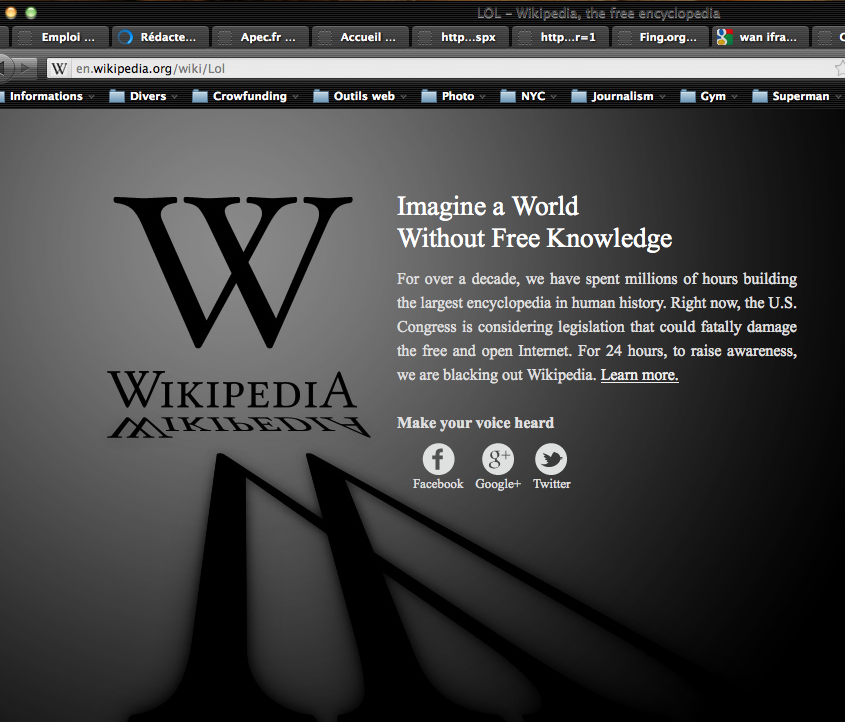
\includegraphics[height=\thumbheight]{sopa/looseduplicate9.png}
    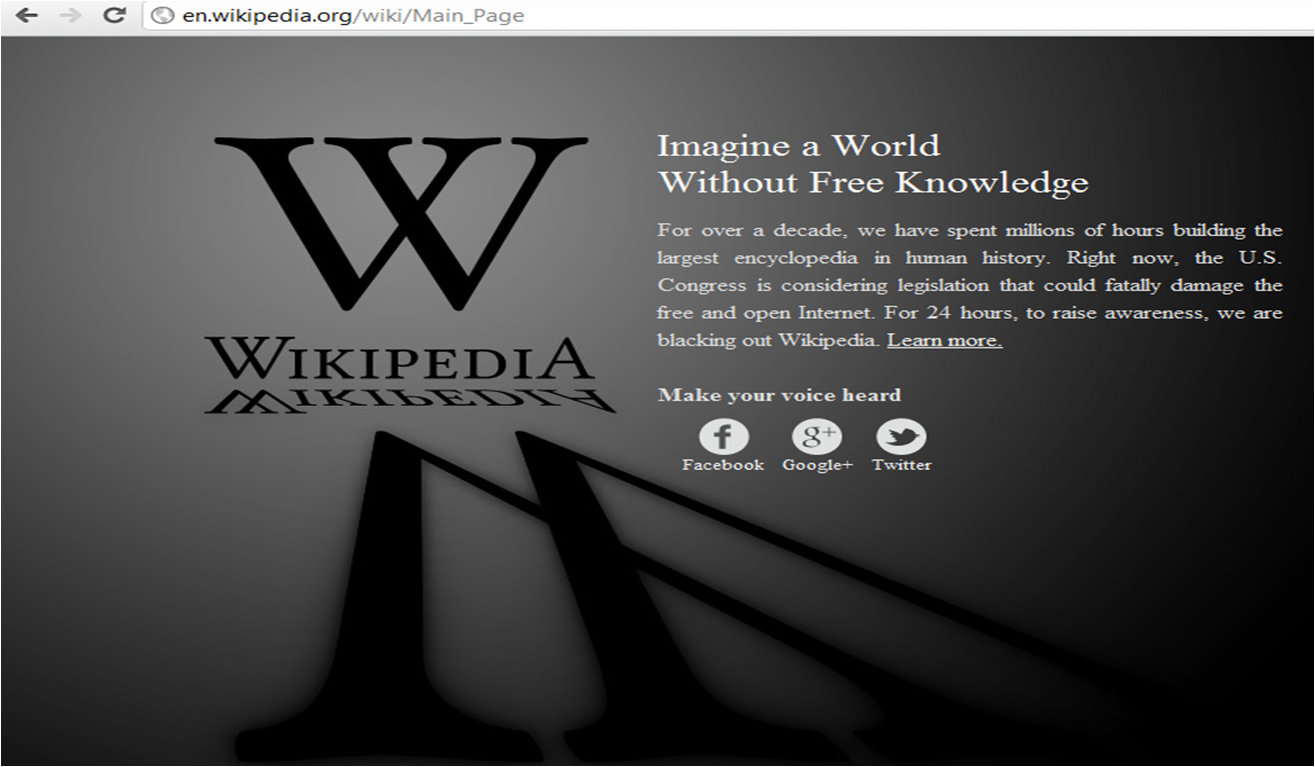
\includegraphics[height=\thumbheight]{sopa/looseduplicate10.png}
    
\includegraphics[height=\thumbheight]{sopa/looseduplicate11.jpg}
    
\includegraphics[height=\thumbheight]{sopa/looseduplicate12.jpg}
  \end{thumbsequence}
  \begin{thumbsequence}
    \setlength\fboxsep{0pt}
    \setlength\fboxrule{0.1mm}
    \fbox{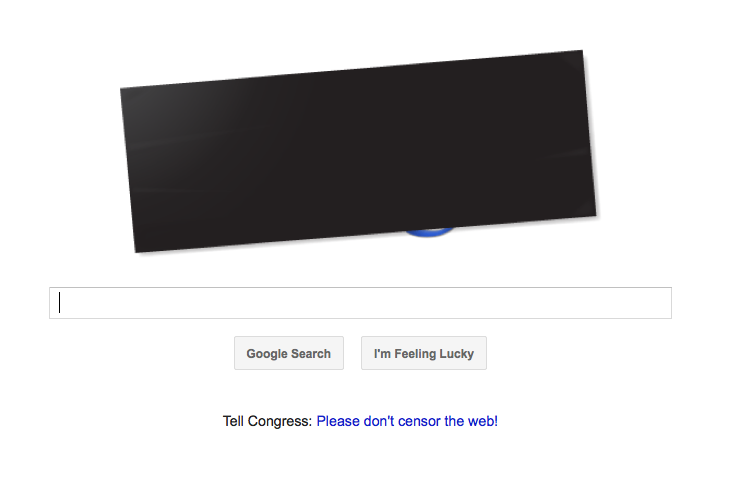
\includegraphics[height=\thumbheight]{sopa/looseduplicate13.png}}
    \fbox{
\includegraphics[height=\thumbheight]{sopa/looseduplicate14.jpg}}
\end{thumbsequence}
\end{tabular}

\begin{tabular}{p{\textwidth}}
\eventtitle{Christian Wulff Case}
  \begin{thumbsequence}
    \doublebox{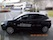
\includegraphics[height=\thumbheight]{wulff/exactduplicate1.jpg}}
    \doublebox{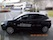
\includegraphics[height=\thumbheight]{wulff/exactduplicate2.jpg}}
  \end{thumbsequence}
  \begin{thumbsequence}
    \doublebox{
\includegraphics[height=\thumbheight]{wulff/exactduplicate3.jpg}}
    \doublebox{
\includegraphics[height=\thumbheight]{wulff/exactduplicate4.jpg}}
  \end{thumbsequence}
\end{tabular}

\begin{tabular}{p{\textwidth}}
\eventtitle{Free Mobile Launch}
  \begin{thumbsequence}
    \doublebox{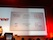
\includegraphics[height=\thumbheight]{free/exactduplicate1.jpg}}
    \doublebox{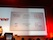
\includegraphics[height=\thumbheight]{free/exactduplicate2.jpg}}
  \end{thumbsequence}
  \begin{thumbsequence}
    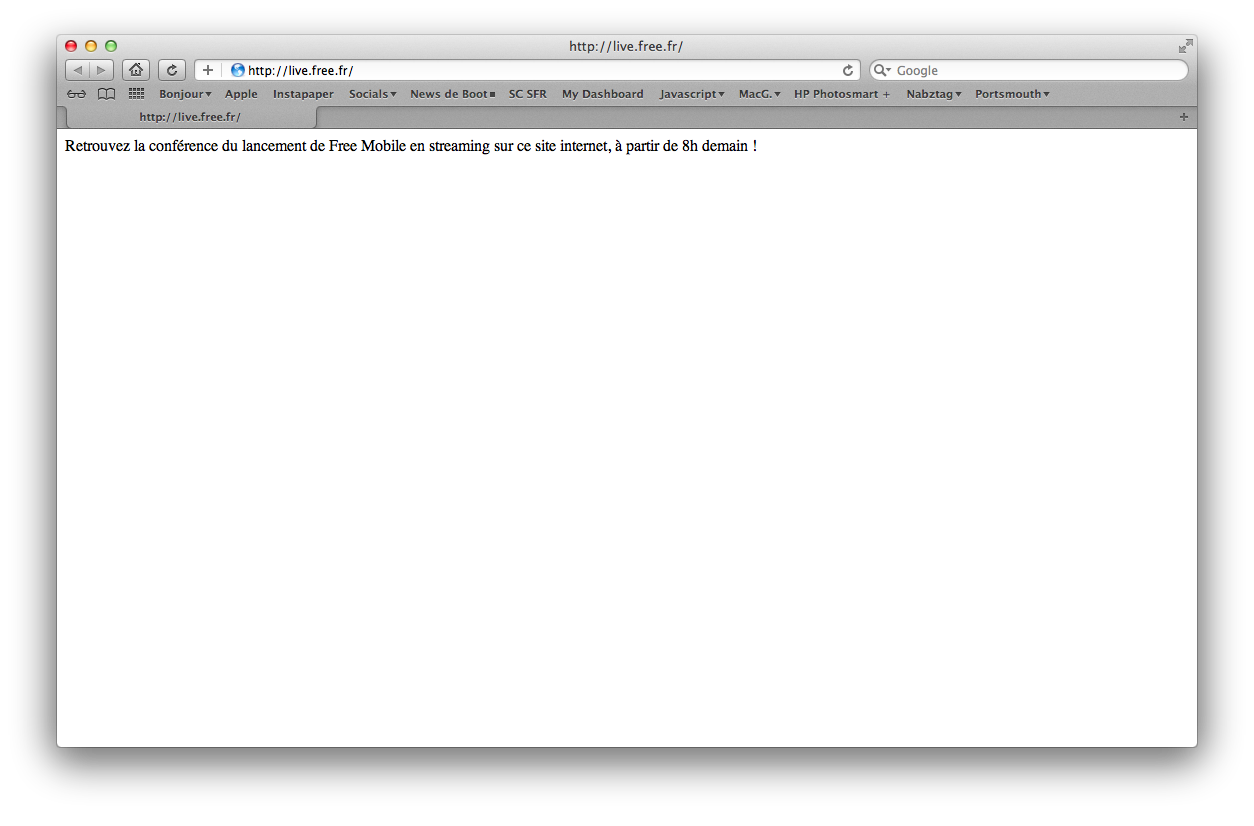
\includegraphics[height=\thumbheight]{free/looseduplicate1.png}
    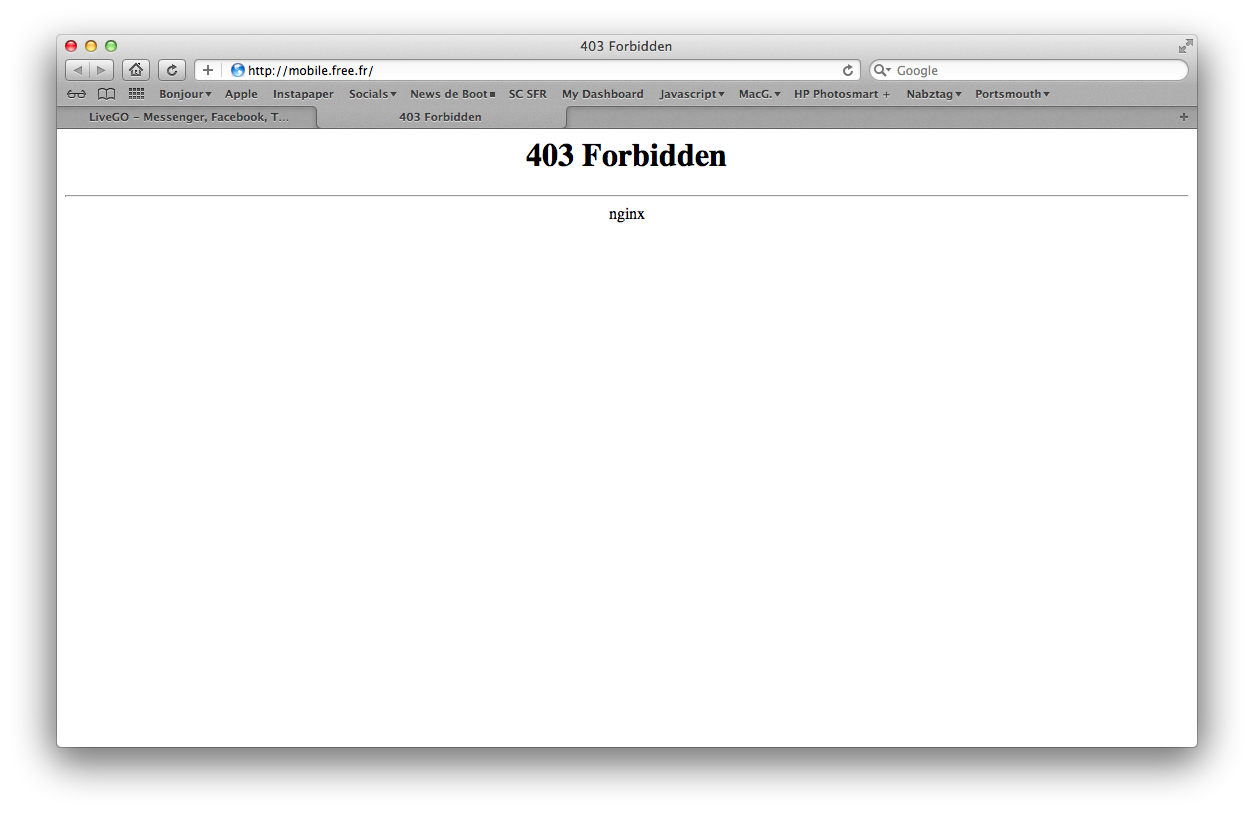
\includegraphics[height=\thumbheight]{free/looseduplicate2.png}
  \end{thumbsequence}
  \begin{thumbsequence}
    
\includegraphics[height=\thumbheight]{free/looseduplicate7.jpg}
    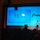
\includegraphics[height=\thumbheight]{free/looseduplicate8.jpg}
  \end{thumbsequence}
  \\[4pt]
  \begin{thumbsequence}
    
\includegraphics[height=\thumbheight]{free/looseduplicate15.jpg}
    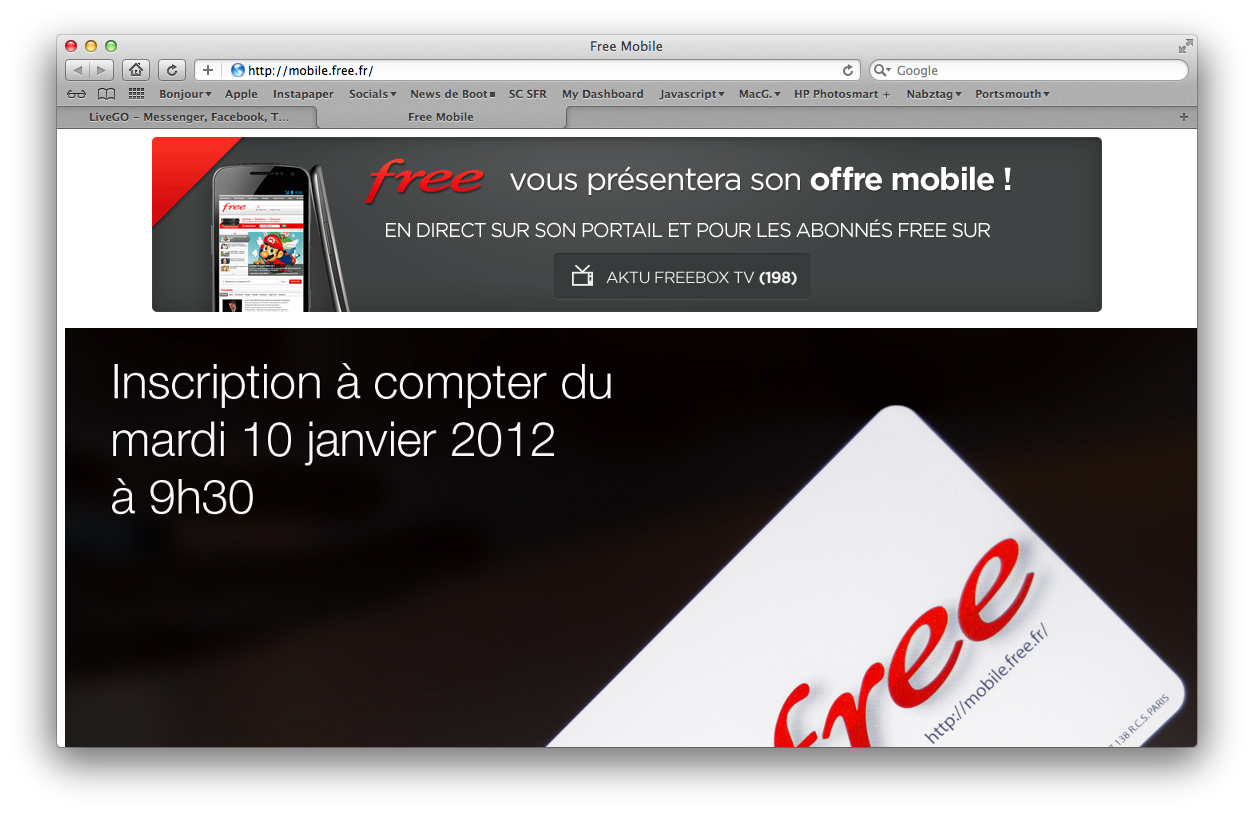
\includegraphics[height=\thumbheight]{free/looseduplicate16.png}
  \end{thumbsequence}
  \begin{thumbsequence}
    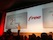
\includegraphics[height=\thumbheight]{free/looseduplicate9.jpg}
    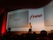
\includegraphics[height=\thumbheight]{free/looseduplicate10.jpg}
    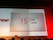
\includegraphics[height=\thumbheight]{free/looseduplicate11.jpg}
  \end{thumbsequence}
  \begin{thumbsequence}
    
\includegraphics[height=\thumbheight]{free/looseduplicate3.jpg}
    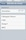
\includegraphics[height=\thumbheight]{free/looseduplicate4.jpg}
  \end{thumbsequence}
  \newstrip
  \begin{thumbsequence}
    
\includegraphics[height=\thumbheight]{free/looseduplicate12.jpg}
    \includegraphics[height=\thumbheight]{free/looseduplicate13.jpg}
    \includegraphics[height=\thumbheight]{free/looseduplicate14.jpg}
  \end{thumbsequence}
  \begin{thumbsequence}
    \includegraphics[height=\thumbheight]{free/looseduplicate5.jpg}
    \includegraphics[height=\thumbheight]{free/looseduplicate6.jpg}
  \end{thumbsequence}
\end{tabular}

\begin{tabular}{p{\textwidth}}
\eventtitle{Costa Concordia Disaster}
  \begin{thumbsequence}
    \includegraphics[height=\thumbheight]{concordia/looseduplicate1.jpg}
    \includegraphics[height=\thumbheight]{concordia/looseduplicate2.jpg}
  \end{thumbsequence}
  \begin{thumbsequence}
    \includegraphics[height=\thumbheight]{concordia/looseduplicate3.jpg}
    \includegraphics[height=\thumbheight]{concordia/looseduplicate4.jpg}
  \end{thumbsequence}
  \begin{thumbsequence}
    \includegraphics[height=\thumbheight]{concordia/looseduplicate5.jpg}
    \includegraphics[height=\thumbheight]{concordia/looseduplicate6.jpg}
  \end{thumbsequence}
\end{tabular}

\begin{tabular}{p{\textwidth}}
\eventtitle{CES Las Vegas}
  \begin{thumbsequence}
    \includegraphics[height=\thumbheight]{ces/looseduplicate1.jpg}
    \includegraphics[height=\thumbheight]{ces/looseduplicate2.jpg}
    \includegraphics[height=\thumbheight]{ces/looseduplicate3.jpg}
    \includegraphics[height=\thumbheight]{ces/looseduplicate4.jpg}
    \includegraphics[height=\thumbheight]{ces/looseduplicate5.jpg}
  \end{thumbsequence}
  \begin{thumbsequence}
    \includegraphics[height=\thumbheight]{ces/looseduplicate6.jpg}
    \includegraphics[height=\thumbheight]{ces/looseduplicate7.jpg}
  \end{thumbsequence}
  \begin{thumbsequence}
    \includegraphics[height=\thumbheight]{ces/looseduplicate8.jpg}
  \end{thumbsequence}
\end{tabular}
\caption[Sample photos for some of the considered nine events]
  {Sample photos for some of the considered nine events
         (showing only exact- or near-duplicate media items)}
\label{fig:sequences}
\end{figure*}


\subsection{The Need for Media Item Deduplication}
\label{sec:the-need-for-media-item-deduplication}

Given our broad approach to retrieve media items
across multiple social networks,
we observed many exact-duplicate or near-duplicate media items.
Oftentimes, these duplicates stem from users who
cross-post to several social networks.
Instead of trying to filter out cross-posted items,
we rather keep them and cluster them.
We are especially interested in social interactions
that media items can trigger.
For example, if one and the same photo
is cross-posted to separate networks,
it can retrieve shares, likes, views, or comments
independently on each of those networks.
By clustering media items, we get a~higher-level view on
a~media item cluster's overall performance on different networks.
We also observed media items that were near-duplicates,
for example, from people who attended the same event like a~concert
and who took photos of the stage from almost the same angle.
Similar to exact-duplicates,
by clustering near-duplicate media items,
we can treat them like exact-duplicates to get the same
network-agnostic viewpoint.
We will examine reasons for exact-duplicate and near-duplicate
media item content and ways to deal with it in \autoref{cha:media-item-deduplication}.

\subsection{The Need for Ranking Media Items}

Our ultimate goal is to generate media galleries
that \emph{visually} and \emph{audially} summarize events.
Especially given high-recall search terms,
we need a~way to rank and prune media items.
Popular media items can be displayed bigger, longer,
or with a~special decoration like a~thicker border
in comparison to less popular media items.
For videos, the audio part poses a~challenge.
In our experiments, we observe that intermixing the audio
of all videos of an event often generates
a very characteristic \emph{noise cloud}
that \emph{audially} conveys the event's atmosphere very well.
A~good example is the Assad Speech event,
where a~mix of Arabic voices blends nicely
with the speech of a~US politician.
A~different example is the CES Las Vegas event,
where the atmosphere of a~big exposition with music,
announcements, and technical analysis becomes alive.
We will have a~closer look at media item ranking in
\autoref{cha:media-item-ranking}.

\section{Conclusions}

In this chapter, we have presented a~generic media extractor
for extracting media items shared on social networks to
illustrate known events.
We have proposed a~common abstraction layer on top of the
social networks' native data formats to align search results.
Our approach to extracting media items and associated
textual microposts covers already most of
the Western world's social networks.
Context-aware multimedia analysis will bring a~new range of
parameters into play since many media items contain a~message
that is complementary to the text.
For example, facial detection~\cite{viola2004facedetection}
and eventually recognition~\cite{wright2009facerecognition}
can signify the presence of specific people in a~media item.
Optical Character Recognition (OCR) can generate
additional textual signals from media items.
As visual recognition systems grow more powerful,
more objects will eventually be recognizable by
machines~\cite{serre2007objectrecognition},
which would allow for generating \emph{visual hashtags}
that describe the content
\emph{inside} of the media item.
Extracted features in all three categories
(\emph{textual}---from the micropost,
\emph{visual}---from the media item,
and \emph{social}---from the social network
in the form of social interactions)
can serve as ranking criteria, be it in isolation
or in combination by introducing a~ranking formula.
As a~result, this will also positively influence
the diversity of automated summarizations.

Nonetheless, it remains important to view the media and the
accompanying microposts as a~whole, since the text
could convey a~sentiment about,
or an explanation of the visual data.
Using named entity recognition as outlined in
\autoref{cha:micropost-annotation},
the important semantic elements in the micropost get identified.
The content of the message can subsequently be used
to narrow down the search space for visual factors
enabling cross-fertilization between the textual
and visual analysis, which results in effective context-aware analysis possibilities~\cite{verborgh2012multimediaannotation,rizzo2012whatfresh}.
Finally, by leveraging the \emph{LOD} cloud,
we can use that knowledge to get a~more diverse view on events.
At time of writing, the so-called
\emph{Operation Pillar of
Defense\footnote{\url{http://en.wikipedia.org/wiki/Operation_Pillar_of_Defense}, accessed July 15, 2013}}
by the Israeli armed forces
causes ongoing conflicts between Palestinians and Israelis.
Using the LOD cloud, promising search terms like, for example,
\emph{gaza}, can be easily looked up in different languages
like Hebrew or Arabic.
In practice, these additional search terms return interesting
new media items that a~pure monolingual search
would not have revealed---oftentimes,
and especially in the concrete case,
at the expense of neutrality.
We are confident that the additional coverage
from more angles helps sharpen one's own viewpoint of an event,
especially with the option of translating microposts
authored in foreign languages,
which is supported by our approach.

\clearpage
\section*{Chapter Notes}
This chapter is partly based on the following publications.
%\cite{rizzo2012whatfresh,khrouf2012aggregatingsocialmedia,khrouf2012confomaton}.

\begin{itemize}
  \interlinepenalty10000
  \item \onlyfullcite{rizzo2012whatfresh}.
  \item \onlyfullcite{khrouf2012aggregatingsocialmedia}.
  \item \onlyfullcite{khrouf2012confomaton}.
\end{itemize}

\clearpage
\printbibliography[heading=subbibliography]
\chapter{Camera Shot Boundary Detection}
\label{cha:shot-boundary-detection}

% the code below specifies where the figures are stored
\ifpdf
    \graphicspath{{7_shot_boundary_detection/figures/PNG/}{7_shot_boundary_detection/figures/PDF/}{7_shot_boundary_detection/figures/}}
\else
    \graphicspath{{7_shot_boundary_detection/figures/EPS/}{7_shot_boundary_detection/figures/}}
\fi

\section{Introduction} \label{sec:videoshotboundarydetection}

In the previous chapter, we have motivated
the need for deduplication of exact-duplicate and near-duplicate media items.
This chapter focuses on camera shot boundary detection,
which is a~first step towards media item deduplication for videos
and photos contained in videos.
In video production and filmmaking, a~\emph{camera shot} is a~series of frames
that runs for an uninterrupted period of time.
Shots are always filmed with a~single camera and can be of any duration.
Shot boundary detection (also called \emph{cut detection},
\emph{shot transition detection},
or simply \emph{shot detection}) is a~field of research of video processing.
Its subject is the automated detection of transitions between shots
with hard or soft cuts as the boundaries
in digital video, with the purpose of temporal segmentation of videos.

In this chapter, we present a~browser-based, client-side, and
on-the-fly approach to this challenge
based on modern HTML5~\cite{berjon2012html5} Web APIs.
Once a~video has been split into shots,
shot-based video navigation becomes possible,
more fine-grained playing statistics can be created,
and finally, shot-based video comparison is possible.
The algorithm developed in the context of our research
has been incorporated in a~browser extension
so that it can run transparently on a~major online video portal.
\autoref{fig:screenshotcamerashots} shows detected camera
shots for a~sample video.

\begin{figure}
\centering
    \includegraphics[height=0.8\textheight,keepaspectratio]{./stevejobs.png}
  \caption[Camera shots for a~sample video on
    a~major online video portal]
    {Camera shots for a~sample video on
    a~major online video portal, detected on-the-fly via
    our shot boundary algorithm incorporated
    in a~browser extension}
  \label{fig:screenshotcamerashots}
\end{figure}

\section{Related Work}

As outlined before, video fragments consist of shots, which are sequences of
consecutive frames from a~single viewpoint,
representing a~continuous action in time and space.
The topic of shot boundary detection has already been described
extensively in literature.
While some specific issues still remain open
(notably detecting gradual transitions and detected false-positives
due to large movement or illumination changes),
the problem is considered resolved for many
cases~\cite{yuan2007shotboundary,hanjalic2002shotboundary}.
Below, we present an overview of several well-known categories of shot boundary detection techniques.

\paragraph{Pixel Comparison Methods:}

Pixel comparison methods~\cite{hampapur1994videosegmentation,
zhang1993videopartitioning} construct a~discontinuity metric
based on differences in color or intensity values
of corresponding pixels in successive frames.
This dependency on spatial location makes this technique
very sensitive to (even global) motion.
Various improvements have been suggested, such as prefiltering
frames~\cite{zhang1995videoparsing},
but pixel-by-pixel comparison methods proved inferior,
which has steered research towards other directions.

\paragraph{Histogram Analysis:}

A~related method to pixel comparison methods is
histogram analysis~\cite{otoole1999shotboundary},
where changes in frame histograms are used
to justify shot boundaries.
Their insensitivity to spatial information
within a~frame makes histograms less prone to partial
and global movements in a~shot.

\paragraph{Hybrid Approaches:}

As a~compromise, a~third group of methods consists of
a~trade-off between the above two
categories~\cite{ahmed1999keyframe}.
Different histograms of several, non-overlapping blocks
are calculated for each frame,
thereby categorizing different regions of the frame
with their own color-based, space-invariant fingerprint.
The results are promising, while computational complexity
is kept to a~minimum, which is why we have chosen
to base our algorithm on a~variation of this approach.

\paragraph{Comparison of Mean and Standard Deviations:}

Other approaches to shot boundary detection include
the comparison of mean and standard deviations
of frame intensities~\cite{lienhart1999comparison}.
Detection using other features such as
edges~\cite{zabih1995scenebreaks} and
motion~\cite{bouthemy1997shotchange} have also been proposed.
Edge detection transforms both frames to edge pictures,
\emph{i.e.}, it extracts the probable outlines of objects.
However, Gargi \emph{et~al.}\ have shown that
these more complex methods do not necessarily
outperform histogram-based approaches~\cite{gargi2000videoshot}.
A~detailed comparison can be found in
Yuan~\emph{et~al.}\cite{yuan2007shotboundary}.

\section{On-the-fly Shot Boundary Detection Algorithm}
\label{sec:details-of-algo}

As outlined in the previous section,
shot boundary detection is mostly considered a~solved problem
and many efficient approaches exist.
However, to the best of our knowledge,
none of the proposed solutions deals with
the specific issue of detecting camera shots in \emph{streaming} video
in the context of a~Web browser and on-the-fly.
Streaming (HTML5) video has no notion of frames,
but only allows for time-based navigation
via the \texttt{currentTime} attribute.
The algorithm we propose in the sequence of this chapter
deals effectively with these limitations
and we also show that it works efficiently.

\subsection{Details of the Algorithm}

In this section, we discuss our shot boundary detection algorithm,
which falls in the category of histogram-based algorithms.
Since visually dissimilar video frames
can have similar global histograms,
we take local histograms into account instead.
We therefore split video frames in freely configurable
rows and columns, \emph{i.e.}, lay a~grid of tiles over each frame.
The user interface that can be seen in \autoref{fig:algorithm}
currently allows for anything from a~$\mathit{1} \times \mathit{1}$
grid to a~$\mathit{20} \times \mathit{20}$ grid.
The limits are imposed by the reasonable processing time on consumer PCs.
For each step, we examine a~frame $\mathit{f}$ and its direct
predecessor $\mathit{f - 1}$ and calculate their tile histograms.
We recall that HTML5 streaming video has no notion of frames,
so by frame we mean a~frame that we have navigated to
via setting the \texttt{currentTime} attribute.
Apart from the per-tile average histogram distance,
the frame distance function further considers
a~freely configurable number of \emph{most different} and
\emph{most similar} tiles.
This is driven by the observation that different parts
of a~video have different intensities of color changes,
dependent on the movements from frame to frame.
The idea is thus to boost the influence of movements in the frame
distance function, and to limit the influence of permanence.
In the debug view of our approach that can be seen in
\autoref{fig:algorithm}, blue boxes indicate movements,
while red boxes indicate permanence.
In the concrete example, Steve Jobs' head and shoulders move
as he talks, which can be clearly seen
thanks to the blue boxes in the particular tiles.
Additional movements come from a~swaying flag on the left,
and a~plant on the right.
In contrast, the speaker desk, the white background,
and the upper part of his body remain static,
resulting in red boxes.
We use a~grid layout of $\mathit{20} \times \mathit{20}$ tiles
($\mathit{nTiles} = \mathit{400}$), and
a~$\mathit{tileLimit = 133 = \mathit{20} \times \mathit{20} * 1/3}$
of most different or similar tiles,
\emph{i.e.}, we treat one third of all tiles
as most different tiles, one third as normal tiles,
and one third as most similar tiles,
and apply boosting and limiting factors to the most different
and most similar tiles respectively.
We work with values of~$\mathit{1.1}$ for the
$\mathit{boostingFactor}$, which slightly increases
the impact of the most different tiles,
and $\mathit{0.9}$ for the $\mathit{limitingFactor}$,
which slightly decreases the impact of the most similar tiles.
These algorithm parameters were empirically determined
to deliver solid results on a~large corpus of videos,
albeit for each individual video the optimal settings
can be manually tweaked to take into account the
particular video's special characteristics.
The algorithm pseudocode can be seen in \autoref{code:algorithm}.

We define the average histogram distance between two frames
$\mathit{f}$ and $\mathit{f - 1}$ as $\mathit{avgHisto_{f}}$.
In a~first step, we have examined the histogram distance
data statistically and observed that while
the overall average frame distance $\mathit{avgDist_{f}}$,
defined as $$\mathit{avgDist_{f}} =
\frac{1}{\mathit{nTiles}}\sum_{t=1}^{\mathit{nTiles}}
\mathit{avgHisto_{f, t}}$$ is very intuitive to human beings,
far more value lies in the standard deviation
$\mathit{stdDev_{f}}$, based on the definition of the overall
average frame distance $\mathit{avgDist_{f}}$
$$\mathit{stdDev_{f}} =
\sqrt{\frac{1}{\mathit{nTiles}}\sum_{t=1}^{\mathit{nTiles}}
(\mathit{avgHisto_{f, t}} - \mathit{avgDist_{f}})^{2}}$$
We use the standard deviation as a~value for the shot splitting
threshold~\cite{lienhart1999comparison}
to obtain very accurate shot splitting results.
We found the boosting and limiting factors to have an overall
positive quality impact on more lively videos
and a~negative quality impact on more monotone videos.
Optimal results can be achieved if,
after changing either the boosting or the limiting factors
for the most similar or different tiles,
the value of the shot splitting threshold is adapted
to the new resulting standard deviation.
The user interface can optionally do this automatically.

\begin{figure}
\centering
    \includegraphics[width=1.0\linewidth]{./algorithm.png}
  \caption[Debug view of the shot boundary detection process]
    {Debug view of the shot boundary detection process.
    Blue boxes highlight tiles with most differences
    to the previous frame, red boxes those with most similarities.}
  \label{fig:algorithm}
\end{figure}

\begin{lstlisting}[caption=Pseudocode of the shot boundary detection
  algorithm,
  label=code:algorithm, float]
for frame in frames
  f = frame.index
  for tile in tiles of frame
    avgHisto[f][tile] = getTilewiseDiff()

  mostDiffTiles = getMostDiffTiles(avgHisto[f])
  mostSimTiles = getMostSimTiles(avgHisto[f])

  for tile in tiles of frame
    factor = 1
    if tile in mostDiffTiles
      factor = boostingFactor
    else if tile in mostSimTiles
      factor = limitingFactor
    avgHisto[f][tile] = avgHisto[f][tile] * factor
  avgDist[f] = avg(avgHisto[f])
\end{lstlisting}

\subsection{Implementation Details}
\label{sec:implementation}

The complete video analysis process happens fully
on the client side.
We use the HTML5 JavaScript APIs of the \texttt{<video>} and
\texttt{<canvas>} tags.
In order to obtain a~video still frame
from the \texttt{<video>} tag at the current video position,
we use the \texttt{drawImage()} function of the 2D context of the
\texttt{<canvas>} tag,
which accepts a~video as its first parameter.
We then analyze the video frame's pixels per tile
and calculate the histograms.
In order to retrieve the tile-wise pixel data
from the 2D context of the \texttt{<canvas>},
we use the \texttt{getImageData()} function.
For processing speed reasons, we currently limit our approach to
a~resolution of one second, \emph{i.e.},
for each analysis step,
seek the video in $\mathit{1s}$ steps.
We then calculate the frame distances as outlined in
\autoref{sec:details-of-algo}.
For each frame, we can optionally generate an \texttt{<img>} tag
with a~base64-encoded data URI representation
of the video frame's data
that can serve for filmstrip representations of the video.

We have implemented the shot boundary detection algorithm
as a~stand-alone Web application and as a~browser extension
for the popular video hosting platform YouTube.
Browser extensions are small software programs that users can install
to enrich their browsing experience with their browser.
They are typically written using a~combination of standard Web technologies,
such as HTML, JavaScript, and CSS.
There are several types of extensions; for this work
we focus on extensions based on so-called \emph{content scripts}.
Content scripts are JavaScript programs that run in the context of Web pages
via dynamic code injection.
By using the standard Document Object Model (DOM)~\cite{lehors2004dom},
they can modify details of Web pages.

\section{Evaluation}

On-the-fly shot detection in streaming video
comes with its very own challenges that were briefly outlined before.
First, it is a~question of streaming speed.
Especially with High Definition (HD) video,
this can be very demanding.
We do not attach the analysis \texttt{<video>} and \texttt{canvas} tags
to the DOM tree~\cite{lehors2004dom} so that the browser
does not have to render them and thus can save some CPU cycles,
however, the video playing logic still has to seek the video position
ahead in one-second steps and process the encountered still frame.
Even on a~higher-end computer (our experiments ran on a~MacBook
Pro, Intel Core 2 Duo 2,66 GHz, 8 GB RAM),
the process of in parallel analyzing and displaying
a~$\mathit{1280} \times \mathit{720}$ HD video of media type
\emph{video/mp4; codecs="avc1.64001F, mp4a.40.2"}
caused an average CPU load of about 70\%.
The HTML5~\cite{berjon2012html5} specification states that
\textit{``when the playback rate is not exactly 1.0,
hardware, software, or format limitations can cause video frames
to be dropped.''}
In practice, this causes the analysis environment
to be far from optimal.
In our experiments we differentiated between false-positives,
\emph{i.e.}, shot changes that were detected,
but not existent, and misses, \emph{i.e.},
shot changes that were existent,
but not detected.
Compared to a~set of videos with manually annotated shot changes,
our algorithm detected fewer false-positives than misses.
The reasons were gradual transitions and shots
shorter than one second (below our detection resolution)
for misses, and large movements in several tiles
for false-positives.
Overall, we reached an accuracy of about 86\%,
which is not optimal, but given the challenges
sufficient for our use case of
detecting near- or exact-duplicate videos.

\section{Future Work}

There is potential for optimization of the analysis speed
by dynamically selecting lower quality analysis video files,
given that videos are oftentimes available in several resolutions,
like Standard Definition (SD) or High Definition (HD).
We have checked in how far analysis results differ
for the various qualities,
with the result that SD quality is sufficient.
We have made the shot detection application available online at
\url{http://tomayac.com/youpr0n/} (accessed July 15, 2013) and invite the reader to compare
the results, \emph{e.g.}, the SD video
\url{http://tomayac.com/youpr0n/videos/vsfashionshow_sd.mp4} (accessed July 15, 2013) with
the HD version \url{http://tomayac.com/youpr0n/videos/vsfashionshow_hd.mp4} (accessed July 15, 2013).

Second, more advanced heuristics for the various user-definable
options in the analysis process are possible.
While there is no optimal configuration for all types of videos,
there are some key indicators that can help categorize videos
into classes and propose predefined known working settings
based on the standard deviation $\mathit{stdDev_{f}}$
and the overall average frame distance $\mathit{avgDist_{f}}$.
Both are dependent on the values of $\mathit{boostingFactor}$,
$\mathit{limitingFactor}$, $\mathit{rows}$, and $\mathit{columns}$.
Interpreting our results, there is evidence
that low complexity settings are sufficient in most cases,
\emph{i.e.}, a~number of $\mathit{rows}$ and $\mathit{columns}$
higher than~$\mathit{2}$ does not necessarily
lead to more accurate shot boundary detection results.
The same applies to the number of to-be-considered most different
or similar tiles $\mathit{tileLimit}$.
We had cases where not treating those tiles differently
at all, \emph{i.e.}, setting
$\mathit{boostingFactor} = \mathit{limitingFactor} = \mathit{1}$,
led to better results; for example with screencast-type videos,
typically used to demonstrate and teach the use of software features
that were not recorded with a~real camera,
but directly recorded from the computer's screen, with ``camera shots''
then later added with video editing software.

\section{Conclusions}

In this chapter, we have introduced an algorithm for video shot boundary detection
that was implemented as a~stand-alone Web application
and as a~browser extension that adds shot boundary detection to YouTube videos.
While the task of shot boundary detection is considered resolved for many cases,
this is not true for the case of streaming online Web video.
With this research, we have proposed and evaluated an approach
that was shown to deliver consistently good results for all sorts of online videos.
The biggest remaining challenge is finding \emph{the} optimal algorithm settings
for a~given video.
Promising directions for improving the shot boundary detection results
are video categorization (fast-moving, slow-moving, color, black-and-white, \emph{etc.})\ prior
to the actual shot detection process.
By publicly sharing our implementation under a~permissive open-source license,
we open the door for future researchers to build upon our current results.

\section*{Chapter Notes}
This chapter is partly based on the following publications.
%\cite{steiner2012shotdetection,steiner2011crowdsourcingevent}.

\begin{itemize}
  \interlinepenalty10000
  \item \onlyfullcite{steiner2012shotdetection}.
  \item \onlyfullcite{steiner2011crowdsourcingevent}.
\end{itemize}

\clearpage
\printbibliography[heading=subbibliography]
\chapter{Media Item Deduplication}
\label{cha:media-item-deduplication}

% the code below specifies where the figures are stored
\ifpdf
    \graphicspath{{8_media_item_deduplication/figures/PNG/}{8_media_item_deduplication/figures/PDF/}{8_media_item_deduplication/figures/}}
\else
    \graphicspath{{8_media_item_deduplication/figures/EPS/}{8_media_item_deduplication/figures/}}
\fi

\section{Introduction}

In \autoref{cha:media-item-extraction},
we have motivated the need for media item deduplication.
By clustering media items, we get a~higher-level view on
a~media item cluster's overall performance on different networks.
As detailed in \autoref{sec:definition}, media items can be
photos or videos.
WordNet~\cite{fellbaum1998wordnet,miller1995wordnet} defines
the term \emph{duplicate} as
\textit{``a copy that corresponds to an original exactly.''}
The corresponding verb \emph{to duplicate} is defined as to
\textit{``make a~duplicate or duplicates of.''}
The derived term \emph{deduplication} in consequence refers to
the act of eliminating duplicate or redundant information.

In this chapter, we will treat video
and photo deduplication separately.
Our goal is to deduplicate media items \emph{on-the-fly}
at the very moment they are extracted from social networks.
Due to this limitation, we cannot rely on any preprocessing
that state-of-the-art algorithms rely on.
Our approaches to video and photo near-duplicate
and exact-duplicate detection are founded
on a~tile-wise histogram-based pixel comparison algorithm
that was partly introduced in the previous chapter.

\subsection{Definitions}

We have defined a~social media item as either a~photo (image) or video
that was \emph{publicly} shared or published
on at least one social network.
In the following, we will use the shorter term media item
rather than the full term and define
what we mean with \emph{duplicate media items} for various cases.

\paragraph{Exact-duplicates for Photos:}

We define two media items of type photo as \emph{exact-duplicates}
if their pixel contents are exactly the same.
This implies that by our definition a~scaled or recompressed version
of the same photo is \emph{not} considered an exact-duplicate.
Similarly, a~rotated version of a~photo is also \emph{not}
considered an exact-duplicate.
In contrast, two photo files with different file names
or different Exchangeable image file
format\footnote{\url{http://www.cipa.jp/english/hyoujunka/kikaku/pdf/DC-008-2010_E.pdf},
accessed July 15, 2013}
(Exif) data are considered exact-duplicate
if their pixel contents are exactly the same.
exact-duplicate photos typically occur if users share content
from one social network on another, for example,
if one user posts a~photo on Instagram that then someone else
(or even the same user) posts on Facebook.

\paragraph{Near-Duplicates for Photos:}

We define two media items of type photo as \emph{near-duplicates}
if their pixel contents differ no more than a~given threshold after resampling.
Examples of near-duplicate photos are scaled versions
of the same photo, photos shot from a~slightly different angle,
rotated photos up to a~certain degree, \emph{etc.}
Near-duplicate photos typically occur if event attendants
stand close to each other and thus take photos
from a~similar standpoint.
Another scenario is when a~user applies a~photo effect to a~photo
(like an Instagram filter) and in the following
shares both the modified
and the unmodified version.

\paragraph{Duplicates for Videos:}

We define two media items of type video as \emph{exact-duplicates}
if their pixel contents are frame by frame exactly the same.
In practice, we lower this condition and instead of every frame
only consider frames at shot boundaries.
We make \emph{no} requirements on the audio, \emph{i.e.},
a~video that has been dubbed in two different languages,
but that fulfills the pixel contents equality condition,
is considered exact-duplicate.
Typical scenarios where exact-duplicate videos can occur is,
for example, two users sharing the same YouTube video
independently from each other.

\paragraph{Near-Duplicates for Videos:}

We define two media items of type video as \emph{near-duplicates}
if their pixel contents per frame differ no more
than a~given threshold.
In practice, we lower this condition and instead of every frame
only consider frames at shot boundaries.
Typical scenarios where near-duplicate videos can occur is through
logo or subtitle insertion, resizing, re-encoding,
or aspect-ration changes.
Note that we do not consider video subsegments near-duplicates,
so a~shortened version of an existing video is considered
different, as a~manual processing step was involved.

\paragraph{Special Case of Photo Contained in a~Video:}

We define the special case of
\emph{a photo being contained in a~video} if the pixel contents
of a~photo media item differ no more than a~given threshold from
the pixel contents of any of the frames of a~video media item.
In practice, we lower this condition and instead of every frame
only consider frames at shot boundaries.
Typically, this phenomenon occurs if two event attendants
of the same event both cover it from almost the same
standpoint, however, if the one attendant takes a~video,
while the other attendant takes a~photo.

\section{Related Work}

Related work in the field of media item deduplication
and clustering can be separated in different areas,
which reflects the grouping of our definitions above.
We further show related work on media fragments,
digital storytelling, and Natural Language Generation,
which we combine for a~novel algorithm debugging approach.

\paragraph{Image Deduplication and Clustering:}

Work on ordinal measures that serve as a~general tool for
image matching was performed by Bhat \emph{et~al.}\
in~\cite{bhat1998imagecorrespondence}.
Chum \emph{et~al.}\ have proposed a~near-duplicate image detection method
using MinHash and term frequency-inverse document frequency (tf-idf)
weighting~\cite{chum2008nearduplicate}.
They use a~visual vocabulary of vector quantized local feature descriptors based on
Scale-Invariant Feature Transform (SIFT)~\cite{lowe1999sift}.
Gao \emph{et~al.}\ \cite{gao2005webimageclustering} have proposed an image clustering method
in the context of Web image clustering, which clusters images
based on the consistent fusion of the information contained in
both low-level features and surrounding texts.
Also in the context of Web pages, Cai
\emph{et~al.}\ \cite{cai2004hierarchicalclustering} have proposed
a~hierarchical clustering method using visual, textual, and link analysis.
Goldberger \emph{et~al.}\ \cite{goldberger2006unsupervisedclustering}
have combined discrete and continuous image models based on a~mixture of Gaussian densities
with a~generalized version of the information bottleneck principle
for unsupervised hierarchical image set clustering.
Chen \emph{et~al.}\ \cite{chen2003cbir} have introduced an image retrieval approach,
which tackles the semantic gap problem by learning similarities
of images of the same semantics.

\paragraph{Video Deduplication and Clustering:}

Specialized methods for video deduplication exist,
for example~\cite{min2011nearduplicatevideo,wu2009nearduplicate}
by Min \emph{et~al.}\ who, given the observation that
transformations tend to preserve the semantic information conveyed
by the video content, propose an approach for identifying
near-duplicate videos by making use of both low-level visual
features and high-level semantic features
detected using trained classifiers.
In~\cite{oliveira2010nearduplicate}, Oliveira
\emph{et~al.}\ report on four large-scale online surveys
wherein they have confirmed that humans perceive videos as near-duplicates
based on both non-semantic features like different image or audio
quality, but also based on semantic features like different
videos of similar content.
A~survey of video deduplication methods has been conducted by
Lian \emph{et~al.}\ in~\cite{lian2010survey}.
In~\cite{guil2007clustering}, Guil \emph{et~al.}\ have proposed a~method
for detecting copies of a~query video in a~videos database
that groups frames with similar visual content while maintaining their temporal order.
In~\cite{okamoto2002videoclustering}, Okamoto \emph{et~al.}\  have proposed an approach
that is based on fixed length video stream segments.
By generating spatio-temporal images, they employ co-occurrence matrices
to express features in the time dimension explicitly.
Yi \emph{et~al.}\ have proposed motion histograms~\cite{yi2005motionhistogram},
where the motion content of a~video at pixel level is represented
as a~Pixel Change Ratio Map (PCRM), which captures the motion intensity,
spatial location, and size of moving objects in a~video.

\paragraph{Image \emph{and} Video Deduplication and Clustering:}

A~method for both images \emph{and} videos
has been proposed by Yang \emph{et~al.}\ \cite{yang2009nearduplicate}.
The authors describe a~system for detecting duplicate images and videos
in a~large collection of multimedia data that uses local difference patterns
as the unified feature to describe both images and videos.
It has been demonstrated that the proposed method is robust against
common image-processing tasks used to produce duplicates.

\paragraph{Media Fragments:}

There are many online video hosting platforms
that have some sort of media fragments support.
In the following, we present two representative ones.
The video hosting platform YouTube%
\footnote{\url{http://www.youtube.com/}}
allows for deep-linking into videos
via a~proprietary URL parameter \texttt{t},
whose value has to match the regular expression
\texttt{\textbackslash d+m\textbackslash d+s} (for minutes and seconds),
as documented in~\cite{youtube2008link}.
Dailymotion\footnote{\url{http://www.dailymotion.com/}}
has similar URL parameters \texttt{start} and \texttt{end},
whose values have to match the regular expression
\texttt{\textbackslash d+} (for seconds).
The CSS Backgrounds and Borders Module Level~3 specification%
~\cite{bos2012css3} defines the \texttt{background-size} property
that can be used to crop media items visually
and thus create the illusion of a~spatial media fragment
when combined with a~wrapping element.
Media Fragments URI~\cite{troncy2012mediafragments}
specifies a~syntax for constructing media fragments URIs
and explains how to handle them
when used over the HTTP protocol~\cite{fielding1999http}.
The syntax is based on the specification of particular name-value pairs
that can be used in URI query strings and URI fragment identifiers
to restrict a~media resource to a~certain fragment.
The temporal and spatial dimensions are currently supported
in the basic version of Media Fragments URIs.
Combinations of dimensions are also possible.

\paragraph{Digital Storytelling:}

Pizzi and Cavazza report in~\cite{pizzi2008debugging}
on the development of an authoring technology
on top of an interactive storytelling system
that originated as a~debugging%
\footnote{Pizzi and Cavazza use the term \emph{debugging}
in the non-IT sense: to check for redundancy, dead-ends, consistency, \emph{etc.}\ in
authored stories.} tool for a~planning system.
Alexander and Levine define in~\cite{alexander2008storytelling}
the term \emph{Web~2.0 storytelling},
where people create \emph{microcontent}---%
small chunks of content, with each chunk conveying a~primary idea---%
that gets combined with social media to form coherent stories.
We use Media Fragments URIs to help human annotators
understand the results of an algorithm
by converting dry software debugging data to digital stories.

\paragraph{Natural Language Generation:}

Natural language generation is the NLP task
of generating natural language from a~machine representation system.
This field is covered in great detail by Reiter and Dale
in~\cite{reiter2000building}.
They divide the task into three stages:
document planning, microplanning, and realization.
\emph{Document planning} determines the content and structure of a~document.
\emph{Microplanning} decides which words, syntactic structures,
\emph{etc.}\ are used to communicate the chosen content and structure.
\emph{Realization} maps the abstract representations
used by microplanning into text.

\section{Photo Deduplication}
\label{sec:photo-deduplication}

We determine the popularity of media items
shared across social networks.
This task involves the deduplication of extracted media items.
In \autoref{cha:shot-boundary-detection}, we have presented an algorithm
for on-the-fly shot boundary detection for video media items.
In this chapter, we will show how components of this algorithm
can be used to deduplicate photos.
Our work is situated in the broader context of summarizing events
based on social network data.
In order to get an overview of a~given event based on a~\emph{potentially large} set
of event-related media items, this set of media items needs to be \emph{pruned}
to exclusively contain highly relevant media items that are as representative
for the event as possible.
Rather than showing the viewer all media items,
clusters of similar media items need to be formed.
Within each cluster, the most representative media item
has to be decided on according to well-defined criteria.
Undesired exact-duplicate or near-duplicate content in the context of social networks
arises in a~number of situations
that we will illustrate in the following.

\subsection{Exact-Duplicate Content}
\label{sec:duplicate-content}

Duplicate content in the context of social networks
arises whenever people either share exactly the same,
or an exact copy of a~given media item.
An example of the latter can be one user uploading the same media item
to the two different social networks \googleplus and Facebook.
An example of the prior can be two users sharing the same
YouTube video independently from each other, or re-sharing each other's content.

\subsection{Near-Duplicate Content}
\label{sec:near-duplicate-content}

Near-duplicate content in the context of social networks
arises in a~number of situations
that we will illustrate in the following.
All photos are real examples of media items shared on social networks
that were clustered correctly as near-duplicates
by our clustering algorithm, which we will detail in
\autoref{sec:near-duplicate-clustering-algorithm}.

\paragraph{Different Viewing Angle:}

When two people attend the same event
and create media items at roughly the same time
covering the same scene,
their media items will be similar
and---the capturing devices' quality aside---only differ in the viewing angles.
\autoref{fig:viewing-angle} shows a~concrete example.

\begin{figure}[!p]
  \centering
  \subfloat[Viewing angle 1]{
    \includegraphics[height=2.7cm]{stage1.jpg}
  }
  \subfloat[Viewing angle 2]{
    \includegraphics[height=2.7cm]{stage2.jpg}
  }
  \caption{Slightly different viewing angles of a~concert stage}
  \label{fig:viewing-angle}
\end{figure}

\paragraph{Logo, Watermark, Lower Third, or Caption Insertion:}

Oftentimes, organizations or individuals insert
logos, watermarks, lower thirds, or captions into media items
to highlight their origin, to convey related information,
or to claim ownership of a~media item.
An example of caption, logo, and lower third insertion
can be seen in \autoref{fig:logo}.

\begin{figure}[!p]
  \centering
  \subfloat[Blank]{
    \includegraphics[width=0.28\textwidth]{speaker1.jpg}
  }
  \subfloat[Caption]{
    \includegraphics[width=0.28\textwidth]{speaker2.jpg}
  }
  \subfloat[Logo, lower third]{
    \includegraphics[width=0.28\textwidth]{speaker3.jpg}
  }
  \caption{Caption, logo, and lower third insertion for a~speaker}
  \label{fig:logo}
\end{figure}

\paragraph{Cropping:}

Cropping refers to the removal of the outer parts of a~media item
to improve framing, accentuate subject matter,
or to (lossily) change the aspect ratio.
Cropping either happens manually via an image editing application
or, more often, by the social networks themselves
to obtain a~square aspect ratio
that better fits the timeline view of users,
as can be seen in the example in \autoref{fig:cropping}.

\begin{figure}[!p]
  \centering
  \subfloat[Original]{
    \includegraphics[height=3cm]{kid1.jpg}
  }
  \subfloat[Cropped]{
    \includegraphics[height=3cm]{kid2.jpg}
  }
  \caption[Original and cropped version of a~photo]
  {Original and cropped version of a~photo (including a~slight color variation)}
  \label{fig:cropping}
\end{figure}

\paragraph{Different Keyframes:}

We have shown an approach to camera shot boundary detection
in \autoref{cha:shot-boundary-detection} and~\cite{steiner2012shotdetection}.
Different frames stemming from the same camera shot
can occur on social networks when preview heuristics
attempt to auto-select a~representative poster frame from a~video with different approaches,
typically resulting in varying frames for different social networks.
\autoref{fig:camera-shot} shows an example of this phenomenon.

\begin{figure}[!p]
  \centering
  \subfloat[Frame 1]{
    \includegraphics[height=3cm]{camera1.jpg}
  }
  \subfloat[Frame 2]{
    \includegraphics[height=3cm]{camera2.jpg}
  }
  \caption[Two different frames stemming from the same camera shot]
    {Two different frames stemming from the same camera shot,
    with the left frame appearing slightly earlier in the video}
  \label{fig:camera-shot}
\end{figure}

\paragraph{Aspect Ratio Changes with Squeezing or Stretching:}

Aspect ratio changes can either happen combined with cropping
(and thus losing parts of the media item) and/or combined with
squeezing or stretching (and thus deforming the media item).
\autoref{fig:bulged} shows an example where a~media item gets stretched.

\begin{figure}[!ht]
  \centering
  \subfloat[Original]{
    \includegraphics[height=3cm]{lordoftherings.jpg}
  }
  \subfloat[Stretched]{
    \includegraphics[height=3cm]{lordoftheringsstretched.jpg}
  }
  \caption{Original and stretched version of a~photo}
  \label{fig:bulged}
\end{figure}

\paragraph{Photo Filters:}

With the raising popularity of Instagram with its 90 million monthly active users,%
\footnote{\url{http://instagram.com/press/}, accessed July 15, 2013}
photo filters that, \emph{e.g.}, emulate retro Polaroid\texttrademark\ or tilt-shift effects
are a~considerable reason for near-duplicate media content on social networks.
\autoref{fig:photo-filter} shows a~typical example.

\begin{figure}[!ht]
  \centering
  \subfloat[Original]{
    \includegraphics[width=0.25\textwidth]{clickclickdecker1.jpg}
  }
  \subfloat[With photo filter]{
    \includegraphics[width=0.25\textwidth]{clickclickdecker2.jpg}
  }
  \caption{Original and version with an applied photo filter of a~photo}
  \label{fig:photo-filter}
\end{figure}

\subsection{Near-Duplicate Photo Clustering Algorithm}
\label{sec:near-duplicate-clustering-algorithm}

In the previous section, we have outlined
reasons and sources for exact-duplicate and near-duplicate content.
In this section, we describe an algorithm tailored to
deduplicating and clustering exact-duplicate and near-duplicate media items.
Design goals for the algorithm include
the capability to detect exact-duplicate and near-duplicate media items
in a~timely, entirely \emph{ad hoc} manner without any pre-calculation.
In general---and especially for big events---event coverage on social networks
is very broad, \emph{i.e.}, there exist more media items
than one could consume in a~reasonable time.
In consequence, it is tolerable for the algorithm to cluster media items aggressively
rather than leaving too many media items unclustered.
The algorithm has a~twofold approach to clustering:
\emph{low-level} analysis by looking at tile-wise pixel data,
combined with \emph{high-level} analysis by detecting faces in media items.
In the following, we describe the face detection component
of our media item clustering algorithm.

\subsection{Face Detection}
\label{sec:face-detection}

Face detection is a~computer vision technology
that determines the regions of faces in media items.
Rotation-invariant face detection aims to detect faces with arbitrary
rotation angles and is crucial as the first step in automatic face detection
for general applications, as face images on social media are seldom upright and frontal.
Face detection is a~subclass of the broader class of object detection.
The Viola-Jones object detection framework proposed in 2001
by Paul Viola and Michael
Jones~\cite{viola2001objectdetection,viola2004facedetection}
provides competitive object detection rates in realtime
and was motivated primarily by the problem of face detection.
We use an algorithm that further improves Viola-Jones,
based on work by Huang \emph{et~al.}\ \cite{huang2007facedetection}
and Abramson \emph{et~al.}\ \cite{abramson2007yef}
in a~JavaScript implementation made available by Liu~\cite{liu2012facedetection}.
This algorithm runs in the context of a~Web browser and,
given the relatively small size of social network media items,
is fast enough to be applied to hundreds of media items
in well less than a~second overall processing time on a~standard laptop
(mid-2010 MacBook Pro, 2.66~GHz Intel Core~2, 8~GB RAM).

\subsection{Algorithm Description}

Our near-duplicate media item clustering algorithm belongs to the family of
tile-wise histogram-based clustering algorithms.
As an additional semantic feature, the algorithm considers detected faces
as described above.
For two media items to be clustered,
the following conditions have to be fulfilled.

\begin{enumerate}
  \item Out of $m$ tiles of a~media item with $n$ tiles ($m \leq n$),
    at most $\textit{tiles\_threshold}$ tiles may differ not more than $\textit{similarity\_threshold}$
    from their counterpart~tiles.
  \item The numbers $f_1$ and $f_2$ of detected faces in both media items
    have to be the same.
    We note that we do not \emph{recognize} faces, but only \emph{detect} them.
\end{enumerate}

\begin{lstlisting}[basicstyle=\ttfamily\scriptsize,caption={[Simplified pseudocode of the deduplication and clustering algorithm]{Simplified pseudocode of the exact- and near-duplicate
  media item deduplication and clustering algorithm}},
  label={code:clustering},escapechar=§]
§\textbf{Input:}§ mediaItems, a list of media items
§\textbf{Output:}§ clusters, a list of clustered media items


§\textit{\# Algorithm settings}§
ROWS = 10
COLS = 10
TILES_THRESHOLD = ceil(ROWS * COLS * 2/3)
SIMILARITY_THRESHOLD = 10


§\textbf{init:}§

§\textit{\# Calculates tile-wise histograms}§
histograms = {}
faces = {}
§\textbf{for}§ item §\textbf{in}§ mediaItems
  faces[item] = getFaces(item)

  histograms[item] = {}
  §\textbf{for}§ tile §\textbf{in}§ item
    histograms[item][tile] = getHistogram(tile)
  §\textbf{end for}§
§\textbf{end for}§



§\textit{\# Calculates tile-wise distances}§
distances = {}
§\textbf{for}§ outerItem §\textbf{in}§ mediaItems
  distances[outerItem] = {}
  §\textbf{for}§ innerItem §\textbf{in}§ mediaItems
    distances[outerItem][innerItem] = {}
    §\textbf{for}§ tile §\textbf{in}§ histograms[outerItem]
      distances[outerItem][innerItem][tile] =
          abs(histograms[outerItem][tile] -
              histograms[innerItem][tile])
    §\textbf{end for}§
  §\textbf{end for}§
§\textbf{end for}§


§\textit{\# Calculates clusters}§
clusters = {}
§\textbf{for}§ outerItem §\textbf{in}§ mediaItems
  clusters[outerItem] = []
  §\textbf{for}§ innerItem §\textbf{in}§ mediaItems
    §\textbf{if}§ outerItem == innerItem §\textbf{then}§ continue
    similarTiles = 0
    distance = distances[outerItem][innerItem]
    §\textbf{for}§ tile §\textbf{in}§ distance
      §\textbf{if}§ distance[tile] <= SIMILARITY_THRESHOLD §\textbf{then}§
        similarTiles++
      §\textbf{end if}§
    §\textbf{end for}§
    §\textit{\# Check condition 1 (tiles)}§
    §\textbf{if}§ similarTiles >= TILES_THRESHOLD §\textbf{then}§
      §\textit{\# Check condition 2 (faces)}§
      §\textbf{if}§ faces[outerItem] == faces[innerItem] §\textbf{then}§
        clusters[outerItem].push(innerItem)
      §\textbf{end if}§
    §\textbf{end if}§
  §\textbf{end for}§
§\textbf{end for}§

§\textbf{return}§ clusters
\end{lstlisting}

The algorithm pseudocode can be seen in \autoref{code:clustering}.
In the actual implementation some speed improvements,
for example, looking up already calculated
distances\footnote{\texttt{distances[outerItem][innerItem] =
distances[innerItem][outerItem]}}
have been applied;
these were omitted in the listing for legibility reasons.
We calculate the histograms and distances only once initially.
The clusters are then recalculated dynamically
whenever either $\textit{tiles\_threshold}$ or $\textit{similarity\_threshold}$ change.
The given values of $\textit{rows} = \textit{cols} = 10$ and
$\textit{tiles\_threshold} = 67 = \lceil \textit{rows} \cdot \textit{cols} \cdot 2/3 \rceil$
and $\textit{similarity\_threshold} = 15$ were determined empirically
on a~large corpus of event-related media items
and are known to deliver solid results.
The corpus has been made available publicly,
see \autoref{sec:evaluation-chpater6} for the details.

\subsection{Experiments}

We have evaluated the near-duplicate photo clustering
on two events from (at time of writing) recent history with high social network coverage
that we will briefly describe in the following.

\paragraph{Grammy Awards Nominations 2013:}

The Grammy Award---or short Grammy---is an award by
the National Academy of Recording Arts and Sciences of the United States
to recognize outstanding achievement in the music industry.
The annual ceremony features performances by prominent artists.
Some of the awards are presented in a~widely viewed televised ceremony.
On December 5, 2012, the nominees for the 55\superscript{th} Annual Grammy Awards
were announced at an event broadcasted live by the broadcast network CBS
titled \emph{Grammy Nominations Concert
Live},\footnote{\url{http://en.wikipedia.org/wiki/2013_Grammy_Awards},
accessed July 15, 2013}
during which Taylor Swift and LL~Cool~J revealed the nominees
in the so-called Big Four categories
Album, Record and Song of the Year, and Best New Artist.
CBS suggested the hashtag \texttt{\#GRAMMYNoms}.

\paragraph{Victoria's Secret Fashion Show 2012:}
\label{sec:vsfashionshow}

The \emph{Victoria's Secret Fashion
Show}\footnote{\url{http://en.wikipedia.org/wiki/Victoria's_Secret_Fashion_Show},
accessed July 15, 2013} is an annual event
sponsored by Victoria's Secret, a~brand of lingerie and sleepwear.
The show features some of the world's leading fashion models
and is used by the brand to promote and market its goods in high-profile settings.
The show is a~lavish event with elaborate costumed lingerie and
varying music by leading entertainers
that attracts hundreds of celebrities and entertainers,
with special performers and acts every year.
The 2012 edition of the show,
which was previously taped on November 7, 2012
was aired on December 4, 2012 on CBS
to an audience of 9.48 million viewers.
CBS suggested the hashtag \texttt{\#VSFashionShow} for the event.

\subsection{Evaluation}\label{sec:evaluation-chpater6}

We have collected and made available%
\footnote{\url{https://www.dropbox.com/sh/2llvjaut32juwrx/7eGLodfP_2},
accessed July 15, 2013}
datasets for both events with
379 photos for the \emph{Victoria's Secret Fashion Show 2012} event
and 949 photos for the \emph{Grammy Awards Nominations 2013} event.
These photos were collected using the media item extraction framework
described in \autoref{cha:media-item-extraction}
using a~mix of hashtag searches with the official event hashtags combined
with full-text searches for event titles and variations thereof~%
\cite{becker2010eventidentification,becker2012plannedevents}.
Due to the short-lived nature of social networks,
the returned results of the media item extraction process itself
are not reproducible.
Additionally, our focus in this chapter
is on media item deduplication and clustering, not extraction.
The concrete clustering parameters for the algorithm were set as listed below.

\begin{enumerate}
  \item $\textit{rows}$ = $\textit{cols}$ = $10$
  \item $\textit{tiles\_threshold}$ = $67$
  \item $\textit{similarity\_threshold}$ = $15$
\end{enumerate}

In the following, we discuss the clustering and deduplication results.
\autoref{fig:topvsfashionshow} and \autoref{fig:topgrammy} show the top clusters
for the \emph{Victoria's Secret Fashion Show 2012} and the
\emph{Grammy Awards Nominations 2013} events respectively.
We then pick some representative examples from both events
and have a~closer look at the clustering algorithm's strengths and weaknesses.

\begin{figure}[!ht]
  \centering
  \includegraphics[width=1.0\linewidth]{./vsfashionshow_clusters.png}
  \caption{Top clusters for the \emph{Victoria's Secret Fashion Show 2012} event}
  \label{fig:topvsfashionshow}
\end{figure}

\begin{figure}[!ht]
  \centering
  \includegraphics[width=0.95\textwidth,height=0.9\textheight,keepaspectratio]{./grammy_clusters.png}
  \caption{Top clusters for the \emph{Grammy Awards Nominations 2013} event}
  \label{fig:topgrammy}
\end{figure}

\paragraph{Algorithm Strengths:}

\autoref{fig:personclose} has a~brunette fashion model in a~pink robe
and a~heart-shaped pink spotlight as central elements of both photos.
Even though the model is shot from different angles and at different times,
the photos are successfully clustered due to the very identifying colors
and the high tile-wise similarity.

\begin{figure}[!ht]
  \centering
  \includegraphics[width=0.4\linewidth]{./person.png}
  \caption{High tile-wise similarity of a~dominating color}
  \label{fig:personclose}
\end{figure}

\autoref{fig:scenecrop} shows two views of a~stage
taken at slightly different times.
The left photo covers a~detail of the scene,
whereas the right photo covers the entire stage.
Due to the tile-wise similarity of the scene detail,
the photos are successfully clustered.

\begin{figure}[!ht]
  \centering
  \includegraphics[width=0.5\linewidth]{./scene.png}
  \caption{Cropped view of a~stage scene}
  \label{fig:scenecrop}
\end{figure}

\autoref{fig:lightingconditions} shows two views of a~stage
under different lighting conditions.
Due to the tile color tolerances and the tile-wise similarity,
the photos are successfully clustered.

\begin{figure}[!ht]
  \centering
  \includegraphics[width=0.5\linewidth]{./viewing_angle.png}
  \caption{Stage and detail of a~stage under different lighting conditions}
  \label{fig:lightingconditions}
\end{figure}

\autoref{fig:zoomed} shows two photos of the same fashion model,
where the left photo is a~zoomed version of the right photo
with added black bars so that the resulting photo
has a~square aspect ratio.
Despite the differences, the photos are successfully clustered.

\begin{figure}[!ht]
  \centering
  \includegraphics[width=0.35\linewidth]{./zoom.png}
  \caption{Zoomed view of a~model with black bars left and right}
  \label{fig:zoomed}
\end{figure}

\autoref{fig:stageperson} shows two views of the same stage,
however, with a~different person.
Due to the dominating tile-wise similarity of the stage tiles,
the photos are clustered.

\begin{figure}[!ht]
  \centering
  \includegraphics[width=0.6\linewidth]{./stage.png}
  \caption{Two views of the same stage with different person}
  \label{fig:stageperson}
\end{figure}

\paragraph{Algorithm Weaknesses:}

\autoref{fig:white} shows five media items with pure white
as the dominating color and a~pure black font
stemming from screenshots of the Grammy results from Web pages.
The algorithm in its previously described form clusters such media items.
This may or may not be desired.

\begin{figure}[!ht]
  \centering
  \includegraphics[width=1\linewidth]{./white.png}
  \caption[Pure white as dominating color stemming from screenshots]
    {Pure white as dominating color stemming from screenshots
    (bad quality caused by down-scaling via the originating social networks)}
  \label{fig:white}
\end{figure}

Likewise, at the other end of the color spectrum,
\autoref{fig:bwtolerance} shows two media items of a~woman
with pure black as the dominating color,
one time with and the other time without added black bars
to fit a~letterbox aspect ratio.
In its previously described form, the algorithm
does \emph{not} cluster such media items
(unless a~very small number $\textit{tiles\_threshold}$
of required similar tiles is selected).
In the majority of cases, though, clustering such media items \emph{is} desired.
Our response to both issues is to ignore a~certain part
of the color spectrum in the algorithm's similarity measure.
In the concrete case, ignoring pure white and pure black correctly fixed
the clustering in our chosen example events in all but one cases,
without negatively impacting previously formed clusters.

\begin{figure}[!ht]
  \centering
  \includegraphics[width=0.55\linewidth]{./bwtolerance.png}
  \caption[Black bars added to fit a~16:9 image in a~4:3 letterbox]
    {Black bars added to fit a~16:9 image in a~4:3 letterbox
    (the white border is part of the original photo)}
  \label{fig:bwtolerance}
\end{figure}

Finally, \autoref{fig:weakness} shows two entirely different media items
that were incorrectly clustered as the tile histograms
were similar enough under the chosen similarity threshold.
The explanation for this is twofold.
First, the original source media items were very small thumbnail-like images,
which hindered face recognition
(there is actually an \emph{unequal} number of faces in each image).
Second, the way the algorithm works
causes the tiles of very tiny media items like the ones in question to blur.

\begin{figure}[!ht]
  \centering
  \includegraphics[width=0.4\linewidth]{./weakness.png}
  \caption{Entirely different photos with similar tile histograms}
  \label{fig:weakness}
\end{figure}

We have experienced in our experiments that there is no single perfect
combination of algorithm parameters,
so the only way to address this issue (besides ignoring too small media items,
which in practice might be the easiest and best solution)
is to make the parameters flexible.
In our graphical user interface, we have created sliders
that let the user interactively preview clustering changes.
As noted before, a~screenshot of the application
is available online at the URL \url{http://twitpic.com/c02qfs/full} (accessed July 15, 2013).

\section{Video Deduplication}

In the previous section, we have introduced
an algorithm for photo deduplication.
In the upcoming section, we will outline the conceptual framework
of how this algorithm can be combined with the previously introduced
video shot boundary detection algorithm from \autoref{cha:shot-boundary-detection}.
This will allows us to on the one hand
directly deduplicate videos on a~shot boundary frame basis
or on the other hand to detect
whether a~given photo is contained in a~video.

\subsection{Photo-contained-in-Video Workflow}

In a~first step, for a~given video, we detect shot boundaries
as described before in \autoref{sec:videoshotboundarydetection}.
To illustrate this,
\autoref{fig:vsfashionshowboundaries} shows an excerpt
of detected shot boundaries for a~video related to
the \emph{Victoria's Secret Fashion Show 2012} event.
The first photo of each shot boundary film stripe
is selected as the particular shot's representative photo.
To detect whether a~given photo stemming from social networks
is contained in the video in question,
the set of extracted shot representative photos is compared
with all social network photos,
some of which are shown in \autoref{fig:topvsfashionshow}.
We note, however, that especially for longer videos
(about 4 minutes and longer)
this approach does not scale due to the sheer number of camera shots
in common videos shared on social networks,
which causes the process to consume too much time in practice.
At the expense of exactness, (the few) poster still frames
that are typically returned by video hosting platform APIs
can be used rather than extracting (all) shot boundaries manually.

\begin{figure}[!ht]
  \centering
  \includegraphics[width=1.0\linewidth]{./vsfashionshowboundaries.png}
  \caption[Excerpt of detected shot boundaries in an event video]
  {Excerpt of detected shot boundaries in a~\emph{Victoria's Secret Fashion Show 2012} event video}
  \label{fig:vsfashionshowboundaries}
\end{figure}

\subsection{Video-contained-in-Video Workflow}

To detect whether a~given video is contained in another,
we follow a~similar approach as outlined in the previous subsection,
with the sole difference being that we need to compare
all detected shot boundary representative photos of the source video
with the ones from the other.
Naturally, this approach is even less scalable
with regard to system response time.
The practicable work-around is, as before, to limit oneself
to poster frames delivered by the video hosting platforms.
Our experiments have shown that this approach works very well
for common social network user behavior.
For example, the 3:19 minutes long video of Mark Zuckerberg explaining
the design and engineering challenges behind Facebook's
recently announced Graph Search product was initially published
on Facebook,\footnote{\url{https://www.facebook.com/about/graphsearch},
accessed July 15, 2013} however, people republished the same video
multiple times on YouTube.
As the YouTube-generated poster frames were similar enough
and even if the other video metadata like title and description
were different, we were able to effectively deduplicate the videos
with the described work-around approach.
We note that this approach works reasonably well
as online videos are still relatively short,
also given that YouTube per default has an (increasable)
limit of 15 minutes per video.%
\footnote{\url{https://support.google.com/youtube/answer/71673?hl=en},
accessed July 15, 2013}

\section[Describing Media Item Differences with Media Fragments URI]{Describing Media Item Differences with Media Fragments URI and Speech Synthesis}

In this section, we describe how media item differences
can be described with media fragments URIs and speech synthesis.
We will combine the two techniques for the purpose of
introducing a~novel algorithm debugging approach,
illustrated with our previously described
media item clustering algorithm.

\subsection{Algorithm Debug View}
\label{sec:algorithm-debug-view}

In order to illustrate the way the algorithm clusters media items,
\autoref{fig:algorithmdebugtwoclusters} shows a~debug view of the algorithm
for two clustered media items related to the
\emph{Grammy Awards Nominations 2013} event.
The red border around the media item indicates at least one detected face.
Independent from the actual media item's aspect ratio,
the tile-wise comparison always happens based on a~potentially squeezed
square aspect ratio version.
The two slightly different media items (caption insertion, lighting change)
were clustered, because out of the $10 \cdot 10 = 100$ tiles,
$85$ of the minimum required $\textit{tiles\_threshold}$ of $67$ tiles differed not more
than the $\textit{similarity\_threshold}$ of $15$ per tile.
In both media items, exactly $1$ face was detected.
A~screenshot of the complete media item clustering application (with a~different event)
is available online at \url{http://twitpic.com/c02qfs/full} (accessed July 15, 2013).

\begin{figure}[!ht]
  \centering
  \includegraphics[width=0.5\linewidth]{./algorithmdebug.png}
  \caption[Algorithm debug view for two clustered media items]
  {Algorithm debug view for two clustered media items
  related to the \emph{Grammy Awards Nominations 2013} event
  (the red border around the media items indicates at least one detected face)}
  \label{fig:algorithmdebugtwoclusters}
\end{figure}

\subsection{Media Fragments Requirements}
\label{sec:media-fragment-requirements}

A~media fragment is a~part that was separated from its parent media item.
In order to make statements about such media fragments,
we need to uniquely identify them.
In the context of our research on media item deduplication and clustering,
media fragments identifiers need to be capable of expressing the following concepts.

\begin{enumerate}
  \itemsep0em
  \item Given a~rectangular media item with the dimensions
    $ width \times height $, express that in turn rectangular
    tiles of smaller dimensions are part of the original media item.
  \item Given detected faces at the granularity level of bounding rectangles,
    express that these bounding rectangles are within the dimensions
    of the original media item and that each bounding rectangle contains a~face.
  \item Requirements \textit{i} and \textit{ii} need to be fulfilled
    for both types of media items, \emph{i.e.}, photos and videos. In case of the latter,
    video subsegments of any length---including video still frames---need to be supported.
\end{enumerate}

Media Fragments URI~\cite{troncy2012mediafragments}
as described in the basic version of the specification
supports all three requirements.
The \emph{temporal dimension} is denoted by the parameter name \texttt{t}
and specified as an interval with a~begin time and an end time.
Either one or both parameters may be omitted,
with the begin time defaulting to 0 seconds
and the end time defaulting to the duration of the source media item.
The interval is half-open: the begin time is considered part of the interval,
whereas the end time is considered to be the first time point
that is not part of the interval.
If only a~single value is present, it corresponds to the begin time,
except for when it is preceded by a~comma,
which indicates the end time.
The temporal dimension is specified in the Normal Play Time
(NPT,~\cite{schulzrinne1998realtime}) format.

The \emph{spatial dimension} selects an area of pixels from media items.
In the current version of the specification,
only rectangular selections are supported.
Rectangles can be specified as pixel coordinates or percentages.
Rectangle selection is denoted by the parameter name \texttt{xywh}.
The value is either \texttt{pixel:} or \texttt{percent:}
(defaulting to \texttt{pixel:}) and four comma-separated integers.
The integers denote $x$, $y$, $width$, and $height$ respectively,
with $x = 0$ and $y = 0$ being the top left corner of the media item.
If \texttt{percent:} is used,
$x$ and $width$ are interpreted as a~percentage of the width of the original media item,
while $y$ and $height$ are interpreted as a~percentage of the original height.
While (at time of writing) the temporal dimension is implemented natively
in common Web browsers, this is not the case for the spatial dimension.

The intent of the Ontology for Media Resources~\cite{lee2012mediaontology}
by Lee \emph{et~al.}\ is to bridge different description methods of media resources
and to provide a~core set of descriptive properties.
Combined with Media Fragments URI, this allows for making statements
about media items and fragments thereof.
An example in RDF Turtle syntax~\cite{prudhommeaux2013turtle}
is given in \autoref{code:media-fragment}.

\begin{lstlisting}[caption={[Description of two 10~sec long media fragments]{Description of two 10~sec long media fragments:
  \textit{(i)}~a~tile of dimensions $ 30 \times 40 $ pixels
  starting at pixel coordinates $ (0, 0) $
  that contains a~face; and
  \textit{(ii)}~a~tile of dimensions $ 10 \times 10 $ pixels
  starting at pixel coordinates $ (0, 0) $ of red color}},
  label=code:media-fragment, float=!ht]
@base <http://example.org/> .
@prefix ma: <http://www.w3.org/ns/ma-ont> .
@prefix foaf: <http://xmlns.com/foaf/0.1/> .
@prefix db: <http://dbpedia.org/resource/> .
@prefix dbo: <http://dbpedia.org/ontology/> .
@prefix col: <http://purl.org/colors/rgb/> .

<video> a ma:MediaResource .
<video#t=,10&xywh=0,0,30,40> a ma:MediaFragment ;
                             foaf:depicts db:Face .
<video#t=,10&xywh=0,0,10,10> a ma:MediaFragment ;
                             dbo:colour col:f00 .
\end{lstlisting}

\subsection{Algorithm Debug Properties}
\label{sec:media-item-deduplication-algorithm}

The deduplication algorithm described in this chapter
belongs to the family of tile-wise histogram-based clustering algorithms.
As an additional semantic feature, the algorithm considers detected faces.
It is capable of deduplicating media items of type video and/or photo.
In the case of video, frames at camera shot boundaries are used.
To illustrate the algorithm debugging mechanics,
we use a~running example of two media items related to a~music video by the
band Backstreet Boys, which can be seen in \autoref{fig:near-duplicate}.
For media items to be clustered,
the following clustering conditions have to be fulfilled.

\begin{description}
  \itemsep0em
  \item[Cond.~1] Out of $m$ tiles of a~media item with $n$ tiles ($m \leq n$),
    the average color of at most $\textit{tiles\_threshold}$ tiles
    may differ not more than $\textit{similarity\_threshold}$
    from their counterpart tiles.
  \item[Cond.~2] The numbers $f_1$ and $f_2$ of detected faces
    in both media items have to be the same.
    We note that the algorithm does not \emph{recognize} faces,
    but only \emph{detects} them.
  \item[Cond.~3] If the average colors of a~tile and its counterpart tile
    are within the black-and-white tolerance $\textit{bw\_tolerance}$,
    these tiles are not considered and $\textit{tiles\_threshold}$
    is decreased accordingly (we will talk about $\textit{effective\_tiles\_threshold}$
    in \autoref{sec:debugging-the-algorithm}).
\end{description}

The black-and-white tolerance $\textit{bw\_tolerance}$ avoids media items
to be clustered when the particular tiles are too dark (\emph{e.g.},
for the video borders in \autoref{fig:near-duplicate}) or too bright (\emph{e.g.},
for screenshots of Web pages or applications, which frequently appear on social networks).
In order to illustrate the way the algorithm deduplicates media items,
\autoref{fig:algorithmdebugtilesimilarity} shows a~debug view of the algorithm
for the two clustered media items related to the previous example
around the \emph{Backstreet Boys} music video.
Independent of the actual media items' aspect ratios,
the tile-wise comparison always happens based on
a~potentially squeezed square aspect ratio version.

\begin{figure}[!ht]
  \centering
  \includegraphics[width=0.9\linewidth]{./backstreetboys.png}
  \caption[\emph{Near-duplicate} music video \emph{Everybody} by the \emph{Backstreet Boys}]{\emph{Near-duplicate} music video \emph{Everybody} by the \emph{Backstreet Boys} shared independently on Facebook and \googleplus}
  \label{fig:near-duplicate}
\end{figure}

\begin{figure}[!ht]
  \centering
  \subfloat[From Facebook user]{
    \includegraphics[width=0.35\linewidth]{debug1.png}
  }
  \subfloat[From Google+ user]{
    \includegraphics[width=0.35\linewidth]{debug2.png}
  }
  \caption[Debug view of the media item deduplication algorithm]{Debug view of the media item deduplication algorithm:
  since no faces are detected in \autoref{fig:near-duplicate},
  the clustering is based on tile similarity;
  pure black tiles are not considered due to the chosen black-and-white tolerance)}
  \label{fig:algorithmdebugtilesimilarity}
\end{figure}

\subsubsection{Debugging the Algorithm}
\label{sec:debugging-the-algorithm}

In this subsection, we consider the following three debug scenarios
that occurred most frequently during our previous experiments with human raters.
They correspond to situations where, given a~set of
deduplicated and clustered media items, a~human annotator wanted
to understand the specific details leading to the decisions
taken by the algorithm that they were unsure about or had decided on differently.

\begin{description}
  \itemsep0em
  \item[Clustering Consent.] Two or more media items are clustered
    by the algorithm and the human rater also agrees.
    The human rater wants to understand why they were clustered.
  \item[Clustering Dissent.] Two or more media items are clustered
    by the algorithm, but the human rater thinks
    that they should not have been clustered.
    The human rater wants to understand why they were incorrectly clustered.
  \item[Non-Clustering Dissent.] Two or more media items are not clustered
  by the algorithm, but the human rater thinks
  that they should have been clustered.
  The human rater wants to understand why they were not clustered.
\end{description}

In order to provide answers to these human raters' information needs,
different levels of the algorithm's internals have to be debugged.
Is the $\textit{tiles\_threshold}$ (\emph{i.e.},
the number of tiles that may differ) too high or too low?
Complementary to this, is the $\textit{similarity\_threshold}$
(\emph{i.e.}, the maximum amount two tiles may differ)
too high or too low (\textbf{Cond.~1})?
Are the number of detected faces $f_1$ and $f_2$ the same?
Are all faces correctly detected, or should the face matching condition
be temporarily disregarded, \emph{e.g.}, with too tiny media items,
where faces fail to be detected (\textbf{Cond.~2})?
If the media items to be compared have very dark and/or very bright parts,
is the $\textit{bw\_tolerance}$ too high or too low (\textbf{Cond.~3})?

\subsubsection{Low-Level Debug Output}
\label{sec:low-level-debug-output}

As a~consequence of the previous observations, the low-level debug output
must include the currently selected $\textit{tiles\_threshold}$ and
$\textit{similarity\_threshold}$ and how many tiles with the present algorithm settings
currently fulfill \textbf{Cond.~1}.
In addition to that, the debug output has to contain
the number of detected faces $f_1$ and $f_2$ in each media item,
\emph{i.e.}, whether \textbf{Cond.~2} is fulfilled,
as well as the number of not considered tiles
(according to $\textit{bw\_tolerance}$), which implies fulfillment of \textbf{Cond.~3}
and potentially impacts \textbf{Cond.~1} in form of
the $\textit{effective\_tiles\_threshold}$.
For instance, consider the low-level debug output for the media items
from the running example of the \emph{Backstreet Boys} media items.

\begin{verbatim}
- Similarity threshold: 15 (Cond. 1)
- Tiles threshold: 67 (Cond. 1)
- Similar tiles: 52 (Cond. 1)
- Faces left: 0. Faces right: 0 (Cond. 2)
- BW tolerance: 1 (Cond. 3)
- Not considered tiles: 22 (Cond. 3)
- Effective tiles threshold: 45 (Cond. 3)
\end{verbatim}

\subsection{From Debug Output to Story}
\label{sec:from-debug-output-to-story}

While this low-level debug output is sufficient to respond
to the polar question (yes/no question) whether media items
are clustered at all or not, it does not help with
the non-polar \emph{why} question
(the linguistic term for this type of questions is \emph{wh–question}).
In order for human raters to get answers to the question on
\emph{why} media items are clustered, we need to lift the low-level debug output
to a~high-level natural language story for
the previously defined debug scenarios \textit{Clustering Consent},
\textit{Clustering Dissent}, and \textit{Non-Clustering Dissent}.
This results in a~natural language generation task,
whose three stages according to Reiter's and Dale's
architecture~\cite{reiter2000building} will be detailed below.

\subsubsection{Generating Natural Language}
\label{sec:text-to-speech-espeak}

\paragraph{Document Planning:}

In our context, the document is a~set of low-level debug data
as illustrated in \autoref{sec:low-level-debug-output}.
The natural language generation task is thus manageable.
We need to convey the currently selected $\textit{tiles\_threshold}$
and $\textit{similarity\_threshold}$, the number of detected faces
$f_1$ and $f_2$ in each media item, and the number of tiles
not considered given the $\textit{bw\_tolerance}$ parameter.

\paragraph{Microplanning:}

The microplanning task is driven by the debug scenarios
that were described previously.
Initially, we need to decide on a~matching condition aspect
of the algorithm that will be first highlighted.
Typically, this will be the overall tiles statistics.
Afterwards, we need to elaborate on secondary matching conditions
such as detected faces and black-and-white tolerance.
The grammatical number (plural or singular)
needs to be taken into account when statements about tile(s) or face(s)
are planned. Some values, \emph{e.g.},
the percentage of matching tiles, are calculated.
The microplanner needs to decide when exactness
(\emph{e.g.},~\textit{``99\% of all tiles''})
and when approximation of calculated values
(\emph{e.g.}, \textit{``roughly 50\%''}) better suits
the human evaluators' information needs. Neutral non-judgmental statements
(\emph{e.g.}, \textit{``45 tiles''}) and biased judgmental statements
(\emph{e.g.}, \textit{``not a~single one [tile]''})
need to be carefully balanced. Finally, in the interest of
a~more naturally sounding phrase composition,
the microplanner needs to be aware of contrasting juxtaposition
(\emph{e.g.}, \textit{``Both the left and the right media item
contain one detected face.''} \emph{vs.}
\textit{``The left media item contains no detected faces,
while the right media item contains one detected face.''}).

\paragraph{Realization:}

We show examples of sentences that are actually generated
for the three different debug scenarios (Quotes~1--3).
For the sake of completeness, we provide one additional example
(Quote~4) for the debug scenario \textbf{Non-Clustering Consent}.
The running example of the \emph{Backstreet Boys} media items
for the music video \emph{Everybody} is represented by Quote~1.

\begin{description}
  \itemsep0em
  \item[Clustering Consent] (Quote~1). \textit{``The two media items
    are near-duplicates. Out of overall 100 tiles,
    52 from the minimum required 45 tiles
    were similar enough to be clustered.
    However, 22 tiles were not considered,
    as they are either too bright or too dark,
    which is a~common source of clustering issues.
    Neither the left, nor the right media item contain detected faces.''}
  \item[Clustering Dissent] (Quote~2). \textit{``The two media items
    are near-duplicates. Out of overall 100 tiles,
    41 from the minimum required 41 tiles were similar enough to be clustered.
    However, 26 tiles were not considered, as they are either too bright
    or too dark, which is a~common source of clustering issues.
    Neither the left, nor the right media item contain detected faces.''}
  \item[Non-Clustering Dissent] (Quote~3). \textit{``The two media items
    are different. Out of overall 100 tiles,
    only 8 from the minimum required 67 tiles
    were similar enough to be clustered. This corresponds to 8 percent of all tiles.
    The left media item contains 2 detected faces,
    while the right media item contains 1 detected face.''}
  \item[(Non-Clustering Consent)] (Quote~4). \textit{``The two media items
    are different. Out of overall 100 tiles, not a~single one
    was similar enough to be clustered. Neither the left,
    nor the right media item contain detected faces.''}
\end{description}

\subsubsection{Technical Implementation}

\paragraph{Text-to-Speech:}

The generated texts are converted to speech using a~text-to-speech system.
We use the eSpeak~\cite{duddington2012espeak} speech synthesizer
that was originally developed by Jonathan Duddington
in a~JavaScript port called Speak.js,
made available by Alon Zakai~\cite{zakai2012speakjs}.
This speech synthesizer uses the formant synthesis method,
which allows for many languages to be provided in a~small size.
Rather than using human speech samples at runtime,
the synthesized speech output is created using additive synthesis
and an acoustic model, where parameters
such as fundamental frequency, voicing, and noise levels
are varied over time to create a~waveform of artificial speech.
The speech is clear and can be used at high speeds.
However, it is not as natural or smooth as larger synthesizers
that are based on speech recordings.

\paragraph{Visual Media Fragments Highlighting:}

We treat and address each tile of a~media item
as a~spatial media fragment. \autoref{fig:similar-different}
shows a~grid of similar, different, and not considered tiles
from the \emph{Backstreet Boys} media items for the \emph{Everybody} music video.
While the speech synthesizer reads the generated text,
the corresponding tiles (\emph{e.g.},~the matching tiles
or the due to the black-and-white tolerance not considered tiles)
are visually highlighted to support the human evaluators' understanding,
as can be seen in \autoref{fig:tile-highlight}
and in a~screencast available at \url{http://youtu.be/DWqwEnhqTSc} (accessed July 15, 2013).
Spatial Media Fragments URIs are currently not implemented
in any common Web browser~\cite{weinberg2013polyfill}.
In order to nonetheless support spatial media fragments,
we use a~so-called JavaScript polyfill for Media Fragments URI
that was developed in the context of this thesis.%
\footnote{\url{https://github.com/tomayac/xywh.js} accessed July 15, 2013}
In Web development, a~polyfill is downloadable code that provides facilities
by emulating potential future features or APIs
that are not built-in to a~Web browser~\cite{sharp2010polyfill}.
Our polyfill---in contrast to an additional earlier
spatial Media Fragments URI polyfill implementation~\cite{weinberg2013polyfill}
by Fabrice Weinberg---supports more browsers and both image \emph{and} video.

\begin{figure}[!ht]
  \centering
  \includegraphics[width=0.75\linewidth]{./similar-different.png}
  \caption[Similar and different corresponding tile pairs]{Similar (upper row) and different (lower row) corresponding tile pairs for the media items from a~Facebook (left column) and a~Google+ user (right column); checkered tiles are not considered due to the black-and-white tolerance}
  \label{fig:similar-different}
\end{figure}

\begin{figure}[!ht]
  \centering
  \includegraphics[width=0.75\linewidth]{./tile-highlight.png}
  \caption[Due to the black-and-white tolerance not considered checkered tiles]{Due to the black-and-white tolerance not considered checkered tiles, as the text-to-speech system explains: \textit{``However, 22 tiles were not considered, as they are either too bright or too dark, which is a~common source of clustering issues.''}}
  \label{fig:tile-highlight}
\end{figure}

\subsection{Evaluation}
\label{sec:evaluation}

\paragraph{Evaluating Natural Language Generation Systems:}

For the evaluation of natural language generating systems,
there are three basic techniques.
First, the \emph{task-based} or \emph{extrinsic} evaluation,
where the generated text is given to a~person who evaluates
how well it helps with performing a~given task~\cite{portet2009nlg}.
Second, there are \emph{automatic metrics}
such as BLEU~\cite{papineni2002bleu}, where the generated text
is compared to texts written by people based on the same input data.
Finally, there are \emph{human ratings}, where the generated text
is given to a~person who is asked to rate the quality and usefulness of the text.
For our evaluation, we have chosen the third approach of human ratings,
as we do not evaluate the natural language generating system in isolation,
but in \emph{combination with a~visual representation}
that makes use of spatial Media Fragments URIs
(\autoref{fig:similar-different} and \autoref{fig:tile-highlight}).

\paragraph{Evaluating Subjective Data:}

A~common subjective evaluation technique
is the \emph{Mean Opinion Score} (MOS,~\cite{itu1998mos}).
Traditionally, MOS is used for conducting subjective evaluations
of telephony network transmission quality,
however, more recently, MOS has also found
wider usage in the multimedia community
for evaluating inherently subjective things
like perceived quality from the users' perspective.
Therefore, a~set of standard subjective tests are conducted,
where a~number of users rate the quality of test samples
with scores ranging from 1 (worst) to 5 (best).
The actual MOS is then the arithmetic mean of all individual scores.

\paragraph{Evaluation Results:}

In the context of this research,
we have conducted MOS test sessions
with five external human raters.
We generated artificially modified deduplicated media item sets
around media items about the \emph{Backstreet Boys}
that were shared on social networks during the time of writing.
These media item sets were curated by yet another independent two external persons,
assisted by a~previously developed software system
that implements the deduplication algorithm described in this chapter.
We asked the two persons to provoke dissent and consent clustering situations
for the five human raters, \emph{i.e.}, obviously correct clustering
(\textbf{Clustering Consent}), obviously incorrect clustering
(\textbf{Clustering Dissent}), and obviously incorrect non-clustering
(\textbf{Non-Clustering Dissent}).
We then asked the five human raters to have the system
automatically explain the algorithm results to them
as described in \autoref{sec:from-debug-output-to-story}.
The raters gave MOS scores ranging from $2$ to $5$,
with the overall average values as follows:
\textbf{Clustering Consent}:~$4.3$, \textbf{Clustering Dissent}:~$3.3$,
and \textbf{Non-Clustering Dissent}:~$4.1$.
The human raters appreciated the parallel explanation approach,
where the visual and the audial parts synchronously described
what the algorithm was doing.
They uttered that the not considered tiles (due to the black-and-white tolerance)
as well as erroneously not detected faces were sources of error
in the algorithm that they easily understood
thanks to the human language description.
They sometimes wished for more diversification in the generated texts.
Without exception, they liked the system and encouraged future development.

\section{Conclusions}

In this chapter, we have treated the topic of media item deduplication
from different angles.
We have first defined the meaning of \emph{exact} and \emph{near-duplicate}
for both photos and videos,
including the special case of a~photo being contained in a~video.
In a~previous chapter,
we have introduced an algorithm and application
for video shot boundary detection
whose foundations then served for a~more general
photo deduplication algorithm with semantic features
in the present chapter.
We have evaluated the algorithm for two recent events
that had broad social media coverage.
Further, we have outlined how the photo deduplication algorithm
can be used for basic video deduplication,
albeit minimum system response time requirements
hinder its full applicability in practice.
Finally, we have successfully demonstrated the feasibility
of making the task of debugging a~complex algorithm
more human-friendly by means of a~combined visual and audial approach.
We have used Media Fragments URI
together with a~natural language generation framework
realized through a~speech synthesizer to visually and audially
describe media item differences.
The approach was successfully evaluated for its helpfulness and utility
with the evaluation method Mean Opinion Score (MOS).
Our contribution also includes a~polyfill implementation
of spatial Media Fragments URIs.

Media item deduplication of both exact- and near-duplicate media items
is a~fundamental step in dealing with huge amounts of social media
and media overload in general.
Highly popular media items not only tend
to retrieve many social interactions on the social network
they were initially shared on, but also on other social networks.
Derivates of popular media items further add noise
to the social media sharing landscape.
Based on our media item deduplication algorithms,
we have contributed effective and efficient tools
to deal with social media overload
and to identify the few needles in the cross network haystack.

\section*{Chapter Notes}
This chapter is partly based on the following publications.
%\cite{steiner2013nearduplicate,steiner2014clustering}.

\begin{itemize}
  \interlinepenalty10000
  \item \onlyfullcite{steiner2013nearduplicate}.
  \item \onlyfullcite{steiner2014clustering}.
\end{itemize}

\clearpage
\printbibliography[heading=subbibliography]
\chapter{Media Item Ranking}
\label{cha:media-item-ranking}

% the code below specifies where the figures are stored
\ifpdf
    \graphicspath{{9_media_item_ranking/figures/PNG/}{9_media_item_ranking/figures/PDF/}{9_media_item_ranking/figures/}}
\else
    \graphicspath{{9_media_item_ranking/figures/EPS/}{9_media_item_ranking/figures/}}
\fi

\section{Introduction}

In the previous chapter, we have introduced methods
to deduplicate exact-duplicate and near-duplicate media items.
In this chapter, we introduce ranking criteria and methods
to put deduplicated media clusters in a~well-defined order.
The application screenshots that can be seen in \autoref{fig:topvsfashionshow}
and \autoref{fig:topgrammy} show the
most intuitive ranking criterion one can imagine (besides publication time):
ranking by occurrence popularity.
The more often a~media item (or a~near-duplicate)
appears in any of the considered social networks,
the higher it should be ranked.
However, ranking by occurrence popularity (or media item cluster size)
disregards one of the most valuable features of social networks:
the social aspects.
In consequence, in this chapter, we will introduce
further media item ranking criteria that,
together with media item cluster size,
allows us to propose more adequate social media item ranking mechanisms.

\section{Media Item Ranking Criteria}

In this section, we describe several criteria that can serve to rank
media items retrieved from social networks.
We base these criteria on the information available via
the media item extractors
described in \autoref{cha:media-item-extraction} and
the deduplication and clustering algorithm
described in \autoref{cha:media-item-deduplication}.
Given event-related search terms,
via these approaches, we extract raw binary media items and associated textual microposts and detected named entities as described in
\autoref{cha:micropost-annotation}
from multiple social networks.

\paragraph{Textual Ranking Criteria:}

This category regards the microposts that accompany media items.
Typically, microposts provide a~description of media items.
Using named entity disambiguation tools,
textual content can be linked to \emph{LOD} cloud concepts~\cite{steiner2011addingmeaning}.
We have described micropost annotation in detail in \autoref{cha:micropost-annotation}.

\paragraph{Visual Ranking Criteria:} \label{sec:visualrankingcriteria}

This category regards the contents of photos and videos.
We distinguish \emph{low-} and \emph{high-level} visual ranking criteria.
High-level criteria include logo detection,
face recognition, and camera shot separation.
Low-level criteria include file size, resolution,
duration of a~video, geolocation, time, and more.
Via \emph{Optical Character Recognition (OCR)}, contained texts can be treated as textual feature.

\paragraph{Audial Ranking Criteria:}

This category regards the audio track of videos.
\emph{High-level} ranking criteria are the presence or absence
of silence, music, speech, or a~mixture thereof in videos.
Similar to visual features before,
audial \emph{low-level} features are the average bit rate,
volume, possibly distorted areas, \emph{etc.}
Through audio transcription, speech can be treated as textual feature.

\paragraph{Social Ranking Criteria:}

This category regards social network effects like shares, mentions,
view counts, expressions of (dis)likes, user diversity, \emph{etc.}
in a~network-agnostic way across \emph{multiple} social networks.
We will detail social aspects later in this chapter.

\paragraph{Aesthetic Ranking Criteria:}

This category regards the desired outcome after the ranking, \emph{i.e.},
the media gallery that illustrates a~given event and its atmosphere.
Studies exist for the aesthetics of
automatic photo book layout~\cite{sandhaus2011photobook},
photo aesthetics \emph{per~se}~\cite{obrador2012photoaesthetics},
and video and music playlist generation~\cite{knees2006musicplaylist,davidson2010videorecommendation}.
However, to the best of our knowledge,
no media gallery composition aesthetics studies exist
that examine mixing video \emph{and} photo media items.

\paragraph{Temporal Ranking Criteria:}

This category regards the publication date of media items.
If media items are clustered, we can use the youngest media item
as cluster representative.
Media items can be ranked by recency, as oftentimes more recent items
are more interesting in the streaming context of social networks.

\section{Social Interactions Abstraction Layer}
\label{sec:social-interactions-abstraction-layer}

As we have described in \autoref{cha:social-networks},
social networks have different paradigms of social interactions.
In \autoref{sec:data-format}, we have briefly presented the overall
abstraction layer on top of the native data formats
of all considered social networks in order to gain
a~network-agnostic view on the underlying social networks.
In this section, we detail the part of the abstraction layer
that models the network-specific social interaction patterns.
Those interaction patterns ideally are exposed by the social network
via specific API calls in order to be considered,
which only is the case for a~subset of the social networks we deal with.
Social interaction data is to some extent the holy grail of social networks,
which is the reason why sometimes Web scraping is the last resort
when not all data is accessible via APIs,
as we have outlined in more detail in \autoref{sec:media-item-extractors}.
In \autoref{table:social-interactions}, we have listed
how we abstract the social interactions in question on each social network.
In our concrete implementation, we differ unknown values
that are returned as \texttt{unknown}, \emph{i.e.},
where the information is not exposed,
from \texttt{0} values, where the value is known to be zero.
We briefly recall the social interactions part
of the abstraction layer's data format:

\begin{description}
  \item[\texttt{socialInteractions}] Container for social
    interactions
  \begin{description}
  \item[\texttt{likes}] Number of times a~micropost was liked, or
    \texttt{unknown}
  \item[\texttt{shares}] Number of times a~micropost was shared, or
    \texttt{unknown}
  \item[\texttt{comments}] Number of comments a~micropost
    received, or \texttt{unknown}
  \item[\texttt{views}] Number of views a~micropost reached, or
    \texttt{unknown}
  \end{description}
\end{description}

\begin{table}[!ht]
  \centering
  \footnotesize
  \begin{tabular}{|l|l|l|l|}
    \hline
    Likes & Shares & Comments & Views\\ \hline
    \pbox[t][4.5cm]{0.2\linewidth}{Facebook Like\\ \googleplus \plusone\\ Instagram Like\\ Flickr Favorite\\ YouTube Like\\ YouTube Favorite\\ Twitter Favorite} & \pbox[t][4.5cm]{0.2\linewidth}{Facebook Share\\ \googleplus Share\\ Twitter ReTweet} & \pbox[t][4.5cm]{0.4\linewidth}{Facebook Comments\\ \googleplus Comments\\ Instagram Comments\\ Twitter manual RT\\ Twitter @Replies\\ Twitpic Comments\\ MobyPicture Comments\\ Flickr Comments} & \pbox[t][4.5cm]{0.2\linewidth}{YouTube Views\\ Flickr Views\\ Twitpic Views\\ MobyPicture~Views}\\
      \hline
    \end{tabular}
    \caption[Abstract social network interaction paradigms]
      {Abstract social network interaction paradigms
      and their underlying native social network counterparts}
  \label{table:social-interactions}
\end{table}

\section{Merging and Ranking}
\label{sec:merging-social-interactions}

If a~set of media items is sufficiently similar to be clustered
under the criteria that were detailed in
\autoref{cha:media-item-deduplication},
we can treat the whole of the cluster
as if it were just one media item.
Therefore, we need to specify a~merging strategy
for the associated data of the individual media items
in the particular cluster.
\autoref{code:merging} shows the pseudocode of the merging algorithm.
During the merging step, we treat unknown values
that are represented as \texttt{unknown} as \texttt{0}.
The alternative to this solution would be to exclude \texttt{unknown} values
from the merging step.
However, as in practice a~considerable amount of
social interaction values are \texttt{unknwon},
we are forced to proceed with the abovementioned simplification.
The algorithm accumulates individual social interactions
and assigns the accumulated values to the cluster.

\begin{lstlisting}[caption=Social interactions merging algorithm,
  label=code:merging, float=!ht, escapechar=§]
§\textbf{Input: cluster}§, cluster of visually similar media items
§\textbf{Output: cluster}§, cluster with merged social interactions

§\textbf{for}§ mediaItem §\textbf{in}§ cluster
  cluster.likes += isUnknown(mediaItem.likes) ? 0 : mediaItem.likes
  cluster.shares += isUnknown(mediaItem.shares) ? 0 : mediaItem.shares
  cluster.comments += isUnknown(mediaItem.comments) ? 0 : mediaItem.comments
  cluster.views += isUnknown(mediaItem.views) ? 0 : mediaItem.views
§\textbf{end for}§

§\textbf{return}§ cluster
\end{lstlisting}

\subsection{Selection of a~Cluster's Visual Representative}

As outlined in the previous section, similar enough media items
are clustered and treated as just one media item
by applying the merging algorithm for the social interactions data.
Now, we introduce an algorithm for the selection of
a~cluster's visual representative.
Naturally, through the way the clustering algorithm works,
the contained media items are already visually similar
based on high-level features.
In consequence, we fall back to using \emph{low-level}
visual ranking criteria as defined in \autoref{sec:visualrankingcriteria}.
\autoref{code:clusterrepresentative} shows the cluster representative
selection algorithm, which is based on the low-level feature photo or video \emph{resolution}.
The algorithm selects the media item with the highest megapixel resolution
as the cluster representative,
which is a~solid heuristic for the optimal photo or video quality.

\begin{lstlisting}[caption={[Pseudocode of the cluster visual representative selection algorithm]{Pseudocode of the cluster visual representative selection algorithm that finds the highest quality media item of a~cluster}},
  label=code:clusterrepresentative, float, escapechar=§]
§\textbf{Input:}§ cluster, cluster of visually similar media items
§\textbf{Output:}§ cluster, cluster with visual representative

maxResolution = 0

§\textbf{for}§ mediaItem §\textbf{in}§ cluster

  §\textit{\# Ensure that videos will always be preferred}§
  §\textbf{if}§ mediaItem.type == 'video' §\textbf{then}§
    mediaItem.width = mediaItem.height = INFINITY
  §\textbf{end if}§

  resolution = mediaItem.width * mediaItem.height
  §\textbf{if}§ resolution >= maxResolution §\textbf{then}§
    maxResolution = resolution
    cluster.representative = mediaItem
  §\textbf{end if}§
§\textbf{end for}§

§\textbf{return}§ cluster
\end{lstlisting}

\subsection{Ranking Formula}
\label{sec:introduction-of-a-ranking-formula}

Up to now, we have shown how media item clusters are formed,
how each cluster's social interactions data is accumulated,
and how a~cluster's representative media item is selected.
In this section, we describe a~ranking formula to rank
a~set of media clusters that match a~given query.
In the ranking formula, we consider several well-defined ranking criteria
that were detailed in~\cite{steiner2012definingaesthetic},
namely visual, audial, textual, temporal, social, and aesthetic.
For a~given set of media item clusters, a~ranking is calculated as shown in the formula below.

\begin{gather}\label{eq:rankingformula}
  \alpha \times \mathit{likes} + \beta \times \mathit{shares} +
  \gamma \times \mathit{comments} + \delta \times \mathit{views} + \nonumber\\
  \epsilon \times \mathit{clusterSize} + \zeta \times \mathit{recency} +
  \eta \times \mathit{quality}
\end{gather}

The factors $ \mathit{likes}, \mathit{shares}, \mathit{comments},$ and $ \mathit{views} $
stem from the individual media items as described in \autoref{sec:social-interactions-abstraction-layer}
and \autoref{sec:merging-social-interactions}.
The factor $ \mathit{clusterSize} $ corresponds to the size of the current cluster.
After some experimentation with different event media items sets,
the factor $ \mathit{recency} $ was empirically determined to be calculated as follows.
If the youngest media item in the cluster is less than or exactly one day old,
the value of recency is 8, for two days it is 4, for three days it is 2,
and for each day more, the value is 1.
The factor $ \mathit{quality} $ is a~representation of the
presence of faces and a~media item's photo or video quality.
Empirically optimized default values
that can be fine-tuned for a~concrete media item set
were determined as follows:
$ \alpha = 2 $, $ \beta = 4 $ , $ \gamma = 8 $, $ \delta = 1 $,
$ \epsilon = 32 $, $ \zeta = 2 $, and $ \eta = 8 $.
These factors follow the usage patterns of the different actions:
viewing happens more often than liking, which in turn happens more often than commenting, \emph{etc.}
We describe the evaluation of the ranking formula in the upcoming section.

\section{Evaluation}
\label{sec-chapter7-evaluation}

Evaluating subjective data like \emph{the} correct ranking
for a~set of media items, is a~challenging task.
For different users, there may be different optimal ranking parameter settings.
A~common subjective evaluation technique
is the previously introduced \emph{Mean Opinion Score (MOS)}~\cite{itu1998mos}.
Given a~subjective evaluation criterion
like the correctness of a~ranking,
MOS provides a~meaningful way to judge the overall quality of our approach.

\subsection{Event Analyses by Social Networks}

We have evaluated our approach with the (at time of writing)
recent event of the Super Bowl XLVII,%
\footnote{\url{http://en.wikipedia.org/wiki/Super_Bowl_XLVII},
accessed July 15, 2013}
which was an American football game between
the American Football Conference champion Baltimore Ravens
and the National Football Conference champion
San Francisco 49ers to decide the National Football League
champion for the 2012 season.
The Ravens defeated the 49ers by the score of 34--31.
This event received broad social media coverage
and the social networks
Twitter, Instagram, and Facebook all published blog posts
with analyses of the event on the respective networks,
whereas the search engine Google
published an analysis of trending queries during the match.
In the following, we provide summaries of these different analyses,
with the expectation to encounter relevant media items
for each of the mentioned highlights in our final ranked list of media items
stemming from the various social networks.

According to Twitter's analysis,%
\footnote{\url{http://blog.twitter.com/2013/02/the-super-tweets-of-sb47.html},
accessed July 15, 2013}
the five moments that generated the most tweets
during the game ordered by decreasing number of tweets per minute were
the power outage,
the 108-yard kickoff return for the Ravens touchdown by Jones,
the moment when the clock expired and the Ravens won,
Jones catches a~56 yard pass for a~Ravens touchdown,
and the Gore touchdown for the 49ers.
Overall, 24.1 million tweets about the game and halftime show were counted,
a~number that even leaves aside the advertisements,
which in recent years have become a~highly expected highlight
of the Super Bowl experience.
The Twitter article further mentions the performance by superstar artist Beyoncé
and a~number of Super Bowl advertisements as highlights of the event.

Instagram's analysis\footnote{\url{http://blog.instagram.com/post/42254883677/sbroundup},
accessed July 15, 2013}
mentions that more than three million photos
with Super Bowl-related terms in their captions were shared and
at peak more than 450 photos about the game were posted every second.
During the halftime show, over 200 photos per second were posted about Beyoncé.
The blog post further highlights how a~TV channel pointed to selected photos
and explains that brands ran Instagram campaigns.
According to Instagram, people used Instagram both directly at the event venue,
but also while watching from home, either by photographing their TV sets,
or by photographing each other how they watched the event.

Facebook's analysis\footnote{\url{http://newsroom.fb.com/News/570/Super-Bowl-XLVII-on-Facebook},
accessed July 15, 2013}
mentions as top five most-talked-about moments of the Super Bowl
the moment when the Ravens won the Super Bowl,
Beyoncé's halftime performance,
the power outage in the Superdome,
Jacoby Jones' 108-yard kickoff return for a~Ravens touchdown, and
Joe Flacco's 56-yard pass to Jacoby Jones for a~Ravens touchdown.
The Super Bowl was nicknamed the Harbaugh Bowl, as both teams' head coaches
are named Harbaugh as last name.
Facebook also mentions Alicia Keys' performance of the National Anthem as special event.

The search engine Google has compiled a~list of top trending search terms
during the match, with the top ones being the sponsor M\&M's, Beyoncé, Baltimore Ravens,
San Francisco 49ers, and Colin Kaepernick (quarterback for the San Francisco 49ers).
Additional spiking search terms were power outage
and Chrysler (driven by an advertisement during the game).
Further advertisement-related search terms were for advertisements for M\&M's,
Mercedes-Benz, Disney's Oz Great and Powerful movie, Lincoln, and Audi.

While (at time of writing) no separate statistics are available
for the video hosting platform YouTube,
Google's blog post mentions that searches for Gangnam Style were trending on YouTube,
along with searches for big game performers
in form of the artists Alicia Keys and Beyoncé.

\subsection{Expected Super Bowl Media Items}

Given the differing social networks' own analyses
that we have summarized in the previous subsection,
we expect to see media items
on at least the following topics (in no particular order)
in our own ranked media item set.

\begin{small_itemize}
  \small
  \item[] the power outage
  \item[] the performances of Beyoncé and Alicia Keys
  \item[] the advertisements
  \item[] the match itself from people at the stadium
  \item[] the Super Bowl watchers around the world
\end{small_itemize}

\autoref{fig:loose_order} and \autoref{fig:strict_order} show media items
for the search bundle \emph{49ers} and \emph{Baltimore Ravens} arranged
in two different media gallery styles, loose order and strict order.
Search bundles are combined separate searches, \emph{i.e.},
we first searched for \emph{49ers} and then for \emph{Baltimore Ravens}
and combined the results as if we had performed just one search.
For details on the automated media gallery generation, we refer the reader to the upcoming
\autoref{cha:media-item-compilation}.

\begin{figure}[!ht]
  \centering
  \includegraphics[width=0.95\textwidth,height=0.88\textheight,keepaspectratio]{loose_order.png}
  \caption[Ranked Super Bowl media gallery in Loose Order, Varying Sizes style]
  {Ranked Super Bowl XLVII media gallery in Loose Order, Varying Sizes~(LOVS) style}
  \label{fig:loose_order}
\end{figure}

\begin{sidewaysfigure}
  \centering  \includegraphics[width=0.95\textwidth,height=0.9\textheight,keepaspectratio]{strict_order.png}
  \caption[Ranked Super Bowl media gallery in Strict Order, Equal Sizes style]
  {Ranked Super Bowl XLVII media gallery in Strict Order, Equal Sizes~(SOES) style}
  \label{fig:strict_order}
\end{sidewaysfigure}

\subsection{Evaluation Approach}

We asked three human raters to agree on a~rating for the media items
that were retrieved for the two queries 49ers and Baltimore Ravens.
We have made the dataset of media items available.%
\footnote{\url{https://www.dropbox.com/sh/30qwuvphcv49max/ilsaMbSdf6},
accessed July 15, 2013}
We then fine-tuned the weight factors
$ \alpha, \beta, \gamma, \delta, \epsilon, \zeta $, and $ \eta $ of the ranking formula
that was introduced in \autoref{sec:introduction-of-a-ranking-formula}
until the highest possible agreement between the human-generated ranking
and the system-generated ranking was reached.
Afterwards, we tested these empirically determined weight factors of the ranking formula
with different events and asked the evaluators to what extent
on a~MOS scale from 1--5 they agreed with each of the top-10 ranked media items.
Rating the ranking of \emph{all} media items is barely possible,
which is why we limit ourselves to rating the top-10 returned results,
a~technique that is also known as \emph{pooling}
in the Information Retrieval community~\cite{liu2009learningtorank}.
Screenshots of some of the events we tested with
and the particular top-ranked media items can be seen in
\autoref{fig:qualcomm}, \autoref{fig:blackberry}, and \autoref{fig:facebookgraphsearch}.

\begin{figure}[!ht]
  \centering
  \includegraphics[width=0.75\linewidth]{facebook.png}
  \caption[Ranked media gallery for the Facebook Graph Search launch event]
  {Ranked media gallery for the Facebook Graph Search launch event
  on January 15, 2013}
  \label{fig:facebookgraphsearch}
\end{figure}

\begin{figure}[!ht]
  \centering
  \includegraphics[width=0.75\linewidth]{blackberry.png}
  \caption[Ranked media gallery for the BlackBerry 10 launch event]
  {Ranked media gallery for the BlackBerry 10 launch event on January 30, 2013}
  \label{fig:blackberry}
\end{figure}

\begin{figure}[!ht]
  \centering
  \includegraphics[width=0.95\textwidth,height=0.88\textheight,keepaspectratio]{qualcomm.png}
  \caption[Ranked media items for the Qualcomm CES 2013 keynote event]
  {Ranked media items for the Qualcomm CES 2013 keynote event
  on January~8, 2013 (raw cluster view)}
  \label{fig:qualcomm}
\end{figure}

\subsection{Evaluation Results}

In this subsection, we present the human raters' results
in the form of MOS scores of the events
that we tested our ranking formula with.
As can be seen in \autoref{table:top-10-mos}
and as the combined MOS of 3.7 (variance 0.8) suggests,
all selected top-10 media items
were overall considered relevant by the human raters.
We arranged for post-test conversations with each human rater
in order to understand their motivations for their ratings.
After talking to the human raters it became clear that
lower scores were mostly caused by outliers in the media item set.
Further discussions with the human raters revealed that
if at a~first glance the context to the event in question was missing,
the raters heavily downgraded the corresponding media items.
We note that in order to test the visual ranking aspect in isolation,
raters were exclusively shown media items
without any micropost context.
This approach made it hard for them to recognize connections
between \emph{remote} media items to events \emph{on-site}.
Examples of remote media items are media items of Super Bowl watchers
around the world or photo montages of online news media
(see Facebook Graph Search launch, BlackBerry~10 launch).
Another reason for outliers according to the raters
were too small media item previews of
videos that only made sense when seen in motion.

\begin{table}
  \centering
  \small
  \begin{tabular}{|l|l|l|l|l|l|l|l|l|l|l|l|l|}
    \hline
    \backslashbox{\textbf{Event}}{\textbf{Rank}} & \textbf{1} & \textbf{2} & \textbf{3} & \textbf{4} & \textbf{5} & \textbf{6} & \textbf{7} & \textbf{8} & \textbf{9} & \textbf{10} & \textbf{avg} & \textbf{var} \\ \hline
    \textbf{Facebook} & 3.8 & 3.3 & 4.9 & 4.2 & 3.9 & 5.0 & 3.7 & 4.8 & 4.8 & 3.1 & \textbf{3.6} & \textbf{0.4}\\ \hline
    \textbf{BlackBerry} & 4.9 & 4.8 & 5.0 & 3.2 & 5.0 & 4.4 & 4.1 & 3.8 & 4.5 & 2.7 & \textbf{3.8} & \textbf{0.8} \\ \hline
    \textbf{Qualcomm}& 4.9 & 4.7 & 4.9 & 5.0 & 2.4 & 4.1 & 3.1 & 5.0 & 2.1 & 3.7 & \textbf{3.6} & \textbf{1.0} \\ \hline
    \textbf{Super Bowl}& 5.0 & 4.1 & 5.0 & 3.2 & 5.0 & 2.8 & 4.1 & 4.6 & 3.3 & 4.0 & \textbf{3.9} & \textbf{0.9} \\
    \hline
  \end{tabular}
  \caption[Mean Opinion Scores (MOS) for top-10 ranked media items]
    {Mean Opinion Scores (MOS) for the top-10 ranked media items of four events (overall MOS: 3.7, variance: 0.8)}
  \label{table:top-10-mos}
\end{table}

\section{Conclusions}

In this chapter, we have detailed criteria
that can be considered for the creation of a~ranking.
We have shown how we abstract social interactions on social networks
and introduced an algorithm to merge social interactions
when media items are clustered.
Additionally, we have detailed an algorithm
for the selection of a~media item cluster's visual representative.
Finally, we have used the previously introduced aspects
for the definition of a~ranking formula
whose weight factors were empirically determined
with a~representative sports event
and successfully evaluated in practice with three other events.
For the task of ranking media items, there is no single one correct solution,
but only optimizations under given constraints.
Albeit a~maximum agreement between human raters is aimed for,
individual users will always have different ranking needs.
With our ranking formula proposition, we want to help
such individual users with a~rationally traceable and useful default ranking
that can be adapted easily to special needs or media item sets.
We have implemented this ranking formula in a~stand-alone application,%
which will be described in more detail in \autoref{sec:socialmediaillustrator}.
With this application,
users can easily modify the weight factors
to see their effects on-the fly.
Besides all possible customization,
the application still proposes reasonable default values
for each individual parameter that have been demonstrated
to work well for the majority of cases.
\autoref{fig:social-media-illustrator} shows a~screenshot of this application
that effectively helps users see the media items needles first
and the haystack last.

\begin{figure}[!ht]
  \centering
  \includegraphics[width=1.0\linewidth]{social-media-illustrator.png}
  \caption[Media item ranking in our application with adjustable weight factors]
  {Media item ranking in our application with adjustable weight factors for the ranking formula}
  \label{fig:social-media-illustrator}
\end{figure}

\clearpage
\section*{Chapter Notes}
This chapter is partly based on the following publications.
%\cite{steiner2013meteoroid,milicic2013live,steiner2013vhsrecording}.

\begin{itemize}
  \interlinepenalty10000
  \item \onlyfullcite{steiner2013meteoroid}.
  \item \onlyfullcite{milicic2013live}.
  \item \onlyfullcite{steiner2013vhsrecording}.
\end{itemize}

\clearpage
\printbibliography[heading=subbibliography]
\chapter{Media Item Compilation}
\label{cha:media-item-compilation}

% the code below specifies where the figures are stored
\ifpdf
    \graphicspath{{10_media_item_compilation/figures/PNG/}{10_media_item_compilation/figures/PDF/}{10_media_item_compilation/figures/}}
\else
    \graphicspath{{10_media_item_compilation/figures/EPS/}{10_media_item_compilation/figures/}}
\fi

\section{Introduction}

In this chapter, we introduce aesthetic principles
for the automated generation of media galleries
based on media items retrieved from social networks
that---after a~ranking and pruning step---can serve to authentically
summarize events and their atmosphere from a~visual
and an audial standpoint.
Mobile devices such as smartphones, together with social networks,
enable people to create, share, and consume media items
like videos or photos.
These devices accompany their owners almost everywhere
and are thus omnipresent at all sorts of events.
At such events---given a~stable network connection---part of
the event-related media items are published on social networks
both as the event happens or afterwards,
once a~stable network connection has been established again.
Ranked media items stemming from multiple social networks
can serve to create authentic media galleries
that illustrate events and their atmosphere.
A~key feature for this task is the semantic enrichment
of media items and associated microposts
and the extraction of \emph{visual}, \emph{audial},
\emph{textual}, and \emph{social} features.
Based on this set of features,
additional \emph{aesthetic} features
can be defined and exploited to obtain appealing
and harmonic media galleries.

\section{Related Work}

While enormous efforts have been made to extract
\emph{visual}, \emph{audial},
\emph{textual}, and \emph{social} features
from media items and microposts on social networks in \emph{isolation},
to the best of our knowledge, remarkably less initiatives
concern the extraction and the application
of all those features \emph{in combination}
for \emph{all} types of media items, including microposts.
In~\cite{sandhaus2011photobook}, Sandhaus \emph{et~al.}\ consider visual and
aesthetic features for the automated creation of photo books.
Obrador \emph{et~al.}\ use visual and aesthetic features
for a~category-based approach to automatically assess
the aesthetic appeal of photographs~\cite{obrador2012photoaesthetics}.
In~\cite{knees2006musicplaylist}, Knees \emph{et~al.}\ use audial and textual
features for the automatic generation of music playlists.
Choudhury \emph{et~al.}\ show in~\cite{choudhury2011sportstweets} how social and textual
features can be used to achieve precise detection results
of named entities and significant events in sports-related microposts.
In~\cite{davidson2010videorecommendation}, Davidson \emph{et~al.}\ show how visual,
textual, and social features can be used for personalized video recommendations.
A service called Storify~\cite{fincham2011storify,atasoy2011storify} lets users manually combine
microposts, photos, videos, and other elements onto one page for the purpose
of storytelling or summarizing an event
and share stories permanently on the Web.
Finally, social networks present photos and videos
often in grid-like galleries,\footnote{\url{http://twitpic.com/904yka/full}, accessed July 15, 2013}
sometimes scaled based on the amount of comments.
When unique media items have been collected,
the remaining task is to summarize events by selecting the most relevant media items or media fragments.
Fabro and B\"osz\"orm\'enyi~\cite{delfabro2012summarization} detail
the summarization and presentation of events from content retrieved from social media.
Nowadays, many domain-specific methods already exhibit good accuracy,
for example, in the sports domain~\cite{li2001sportsvideo,li2010americanfootball}. However, the challenge is to find content-agnostic methods.
Methods that exploit semantic information~(\emph{e.g.},~\cite{chen2009videosummarization})
will likely provide high-quality results in the near future,
but today's most relevant summaries are still produced by
manual---at best semi-automated---user interaction~\cite{olsen2011videosummarization}.

\section{Media Gallery Aesthetics}

\paragraph{Definition:}

A media gallery is a~compilation of photos or videos
retrieved from social networks that are related to a~given event.
Given a~set $M_{start} = \{m_1,..., m_n\}$ of media items related to a~certain event,
a~ranking formula $f$, and a~ranking threshold $t$,
the resulting subset $M_{final} \subset M_{start}$
is the result after the application of $f$ to $M_{start}$: $f(M_{start})=M_{ranked}$
and pruning the ranked set $M_{ranked}$ to only include members
whose rank is greater than $t$, with the resulting set named $M_{final}$.
Each media item $m_i$ can either be an instance of video or photo.
For each point $t_x$ on a~timeline $T$, the state of the media gallery
at $t_x$ is defined for each media item $m_i$
as a~set $S_x$ of $n$ tuples $s_{x,i}$, where
$s_{x,i}=\langle \mathit{left}$, $\mathit{top}$, $\mathit{width}$, $\mathit{height}$,
$\mathit{alpha}$, $\mathit{z\mbox{-}index}$, $\mathit{animation}$,
$\mathit{start}$, $\mathit{playing}$, $\mathit{volume} \rangle$.
The first six properties are defined as in CSS~%
\cite{bos2011css}, the $\mathit{animation}$ property
allows for the definition of CSS transitions as defined in~%
\cite{jackson2013csstransitions}
and CSS transformations as defined in~%
\cite{fraser2012csstransforms},
the $\mathit{start}$ property defines the start time in a~video.
The property $\mathit{playing}$ describes whether a~video is currently paused or playing.
Finally, the property $\mathit{volume}$ describes the volume level
of a~video.
A schematic media gallery at $t_x$ can be seen in \autoref{fig:media-gallery}.

\begin{figure}[!ht]
  \centering
  \includegraphics[trim=20mm 40mm 20mm 10mm, clip, width=0.7\columnwidth]{media-gallery.pdf}
  \caption{Schematic media gallery with four photos and two videos}
  \label{fig:media-gallery}
\end{figure}

\paragraph{Audial aesthetics:}

Audial aesthetics thus consist of aspects like volume level normalization,
avoiding multiple videos playing music in parallel, smooth transitions, \emph{etc.}
We remark that through selective mixing of audio tracks
of event-related videos, ``noise clouds''
that are very characteristic
for an event's atmosphere can be observed.
We support this by allowing users to play more than one video at a~time.

\paragraph{Visual aesthetics:}

Visual aesthetics are determined by the composition, \emph{i.e.},
the relation of the number of photos \emph{vs.} the number of videos \emph{globally},
\emph{per coherent scene}, and per \emph{point in time}.
In order to avoid cognitive overload of viewers,
the number of visible (moving) media items
at a~time should be limited.
We will treat this topic in more detail in \autoref{sec:user-studies}.
Depending on the event,
a~consistent or a~contrast-rich overall
appearance and transitions of items may be desired.

\section{Motivation for Automated Media Gallery Generation}
\label{sec:motivation-chapter-8}

Media galleries (see \autoref{fig:media-gallery1} and \autoref{fig:media-gallery2}
for examples)
help users consume significant
amounts of media items in an ideally pleasing and aesthetic way.
These media items may---or, more commonly: may not---be ordered,
besides an intrinsic chronologic order.
In the context of our work on summarizing events
based on microposts and media items stemming from
multiple social networks, we have created methods
to first \emph{extract} event-related media items
from multiple social networks, second, to
\emph{deduplicate} near- and exact-duplicate media items,
third, to \emph{cluster} them by visual similarity, and
finally, to \emph{rank} the resulting media item clusters
according to well-defined ranking criteria.
In this chapter, we treat the challenge of \emph{compiling}
ranked media item clusters in media galleries in ways
such that the ranking-implied order is at least loosely respected.
In the previous section, we have defined
aesthetic principles for automated media gallery layout~\cite{steiner2012definingaesthetic},
which we now apply to media gallery styles.
The task of media gallery compilation is different
from the widely researched task of photo book generation,
as media galleries can contain both photos and videos.
Different types of media gallery layouts are possible,
two of which we have implemented and evaluated via two different user studies:
one with, and one without detailed user comments.

\section{Media Gallery Styles}
\label{sec:mediagallerystyles}

Media galleries---in contrast to free-form digital media collages---%
necessarily display media items in a~grid-like way.
The crucial question is thus whether the media items' aspect ratios
should be respected, or whether they should be cropped to square,
or other aspect ratios (\emph{e.g.}, 4:3 or 16:9).
Respecting the aspect ratio has the advantage that media items
do not need to be cropped, which may affect important contained information like, \emph{e.g.},
contained faces or text.
However, due to the unpredictable media item formats,
compiling media galleries that do not look frayed is harder.
The advantage of cropping is that media gallery layout is easier,
as the media item formats are predictably the same,
at the cost of having to decide where to crop.
Different algorithms (\emph{e.g.},~\cite{suh2003thumbnail})
beyond this chapter's scope exist to aid this decision.
Common cropping heuristics include
maximizing the number of included faces,
focusing on the detected center of the media item,
or cropping at detected background areas.


\paragraph{Terminology:}

We use the following terminology.
A~media gallery is called \emph{balanced} if its shape is rectangular,
\emph{hole-free} if there are no gaps from missing media items,
and \emph{order-respecting}
if media items appear in insertion order.
Optimal media galleries fulfill all three conditions.

\paragraph{Non-Order-Respecting Styles:}

An interesting technique for arranging media items is dividing.
Paper sizes that follow the ISO~216 standard%
\footnote{\url{http://www.iso.org/iso/iso_catalogue/catalogue_tc/catalogue_detail.htm?csnumber=36631},
accessed July 15, 2013}
are the most common every-day examples of the dividing principle:
every media item with an aspect ratio of $ \sqrt2 $ can be divided
into two media items with the same aspect ratio%
~\cite{chedeau2012lightboxandroid}.
This works for portrait and landscape orientations,
however, is not necessarily order-respecting.
Two other non-order-respecting techniques are (i)~%
working with pre-defined placeholder patterns
(small and big squares, portrait and landscape rectangles)
and then filling the placeholder shapes with media items%
~\cite{chedeau2012500px}
or (ii)~working with columns of pre-defined widths
and then iteratively inserting in the smallest column%
~\cite{chedeau2012lightbox}.

As outlined in \autoref{sec:motivation-chapter-8},
we require (at least loosely) order-respecting media galleries
for the ranking step to make sense.
In the upcoming two paragraphs, we will introduce two techniques
for the generation of such media galleries.

\paragraph{Strict Order, Equal Size (SOES):}

A~media gallery style that we call \emph{Strict Order, Equal Size (SOES)},
which strictly respects the ranking-implied order is presented in~%
\cite{chedeau2012googleplus}.
Examples can be seen in \autoref{fig:a} and \autoref{fig:c}.
The algorithm works by resizing all media items in a~row to the same height
and adjusting the widths in a~way that the aspect ratios are maintained.
A~row is filled until a~maximum row height is reached,
then a~new row (with potentially different height) starts, \emph{etc.}
This media gallery style is strictly order-respecting, hole-free,
and can be balanced by adjusting the number
of media items in $+1$ steps.

\begin{figure}[!ht]
  \centering
  \subfloat[\emph{SOES}, Survey~A]{
    \includegraphics[height=5cm]{equal-size.png}
    \label{fig:a}
  }
  \subfloat[\emph{LOVS}, Survey~A]{
    \includegraphics[height=5cm]{different-size.png}
    \label{fig:b}
  }
  \caption[Survey~A: Media galleries visualizing a~gathering at Times Square]{Survey~A: Media galleries visualizing a~gathering at Times Square, New York on February 8, 2013}
  \label{fig:media-gallery1}
\end{figure}

\begin{figure}[!ht]
  \centering
  \subfloat[\emph{SOES}, Survey~B]{
    \includegraphics[height=5cm]{timessquare_2.png}
    \label{fig:c}
  }
  \subfloat[\emph{LOVS}, Survey~B]{
    \includegraphics[height=5cm]{timessquare_1.png}
    \label{fig:d}
  }
  \caption[Survey~B: Media galleries visualizing a~gathering at Times Square]{Survey~B: Media galleries visualizing a~gathering at Times Square, New York on February 8, 2013}
  \label{fig:media-gallery2}
\end{figure}

\paragraph{Loose Order, Varying Size (LOVS):}

Examples of a~media gallery style
that we call \emph{Loose Order, Varying Size (LOVS)}
can be seen in \autoref{fig:b} and \autoref{fig:d},
with the details explained in~\cite{chedeau2012facebook}.
The algorithm works by cropping all images to a~square aspect ratio,
which allows for organizing media items in a~way such
that one big square always
contains two horizontal blocks, each with two pairs of small squares.
The media gallery is then formed by iteratively filling
big or small squares until a~square is full
and then adding the square to the smallest column.
This media gallery style allows any media item to become big,
while still being loosely order-respecting and always hole-free.
Balancing the gallery is slightly harder,
as depending on the shape both small \emph{and} big
media items may be required.

\subsection{Discussion and Evaluation}
\label{sec:user-studies}

The main motivation for the \emph{Loose Order, Varying Size} style
is that certain media items can be featured more prominently
by making them big, while still loosely respecting the ranking-implied order.
Examples of to-be-featured media items can be videos,
media items with faces, media items available in High-Density quality,
or media items with interesting details~%
\cite{suh2003thumbnail}.
Users may want to decide what media items to feature,
albeit we aim for an automated solution.
Evaluating subjective data like \emph{the} correct presentation form
for a~set of media items is a~challenging task.
For different users and different media galleries,
there may be different optimal settings.
Again, we use the Mean Opinion Score (MOS,~\cite{itu1998mos})
for our evaluation, as previously motivated.

\paragraph{User Studies:}

We have conducted two types of surveys.
Survey~A via multiple social networks, where we simply asked people to ``Like''
and/or comment on their favorite style of media gallery
and Survey~B that was distributed via email to a~company-internal ``miscellaneous'' mailing list,
where we asked people to rate media galleries via MOS, with optional comments.
Survey~A and Survey~B used different media items in the media galleries,
as to have some measure in how far content has an impact.

\paragraph{Survey A---Via Social Networks:}

For Survey~A on the social networks Twitter, Facebook,
and \googleplus, we had overall 16~participants (7~female, 8~male, 1~unknown).
7~users liked \emph{SOES} more,
whereas 9~users liked \emph{LOVS} more.
Interestingly, no user commented on why they liked \emph{SOES} more.
Users who commented on why they liked \emph{LOVS} more mentioned
they liked the additional structure and tidiness,
the fact that some media items were bigger,
the fact that it was easier to identify individual media items,
and the fact that important media items were highlighted.

\paragraph{Survey B---Via Email:}

For Survey~B via email with MOS ratings,
we had 19~participants (6~female, 13~male).
The majority of users who liked \emph{LOVS} more
mentioned that the different sizes
gave the eye focal points and orientation,
whereas one user explicitly disliked this guidance.
Users liked the harmony and the structure.
Two users mentioned that small media items were proportionally too small.
Regarding \emph{SOES}, users reported they felt overloaded
and did not know where to start.
Some users said the layout was boring and that,
while they liked the outer framing,
they were confused by the irregular inner grid.
The MOS for \emph{SOES} was $2.39$ (variance $0.68$),
the MOS for \emph{LOVS} was $4.17$ (variance $0.47$).
The data of Survey~B is available.%
\footnote{\url{http://bit.ly/media-gallery-survey},
accessed July 15, 2013}
For privacy reasons, we have posted the media galleries
as non-public microposts on social networks,
which is why we are unable to share the data of Survey~A.

\subsection[Maintaining Provenance Information with Media Galleries]{Maintaining Provenance Information with Downloadable Media Galleries}

Media galleries consist of individual media items,
each with its specific pieces of provenance data
like creator, originating social network, \emph{etc.}
In the context of the application that we have developed
in the context of this thesis and
that will be described in full detail in \autoref{sec:socialmediaillustrator},
this provenance data is maintained in the form of HTML hyperlinks
back to the originating social networks.
However, when media galleries get downloaded in form of
one static image dump, this is no longer the case.
In consequence, we generate a~caption-like image legend
that gets added to each downloaded media gallery.
An example of a~media gallery with provenance data
generated in the context of the 2013 Taksim Gezi Park protests%
\footnote{\url{http://en.wikipedia.org/wiki/2013_Taksim_Gezi_Park_protests},
accessed July 15, 2013}
can be seen in \autoref{fig:occupygezidump}.

\begin{figure}[!ht]
  \centering
  \includegraphics[width=0.9\columnwidth]{occupygezidump.png}
  \caption{Downloadable media gallery with provenance data}
  \label{fig:occupygezidump}
\end{figure}

\section{Interactive Media Galleries}
\label{sec:interactivemediagalleries}

\paragraph{Traditional slideshows:}

Up to now, we have presented different algorithms
to generate media galleries of different styles
and static media galleries, including a~way to preserve
provenance data when media galleries get downloaded as one image.
Such media galleries are useful in the context of static media,
such as newspapers or embedded in (online or offline) news articles.
A~first step towards more interactive media galleries are so-called slideshows.
An exemplary slideshow, courtesy of the BBC's Online division, can be seen in \autoref{fig:occupygezibbc}.

\begin{figure}[!ht]
  \centering
  \includegraphics[width=0.8\columnwidth]{occupygezibbc.png}
  \caption[Media gallery in form of a~slideshow]{Media gallery in form of a~slideshow
  (Source and copyright: BBC Online \url{http://www.bbc.co.uk/news/world-europe-22740038}, accessed July 15, 2013)}
  \label{fig:occupygezibbc}
\end{figure}

\paragraph{Media gallery paradigm slideshows:}

We have opted to extend the traditional slideshow model
by adhering to the media gallery paradigm of our two preferred styles
Loose Order, Varying Size (\emph{LOVS}) and Strict Order, Equal Size (\emph{SOES}).
Given a~media gallery in either \emph{LOVS} or \emph{SOES} style,
each media item can be focused,
\emph{i.e.}, be put prominently in the foreground.
When a~media item is focused, it smoothly transitions
from its original location in the media gallery to the center,
while in parallel it is zoomed to double its size.
All other media items that are currently not focused are faded out
in a~black-and-white variant and blurred, in order to put the maximum emphasis
to the currently focused media item.
\autoref{fig:interactive-media-gallery} shows three steps of the described transitions and
\autoref{fig:occupygezi1} shows the final state after the transition.
A~short screencast of the whole animation is available online
at the URL \url{https://vine.co/v/bT7eiwjE6DQ} (accessed July 15, 2013).

\begin{figure}[!ht]
  \centering
  \subfloat[Animation step 1]{
    \includegraphics[height=4cm]{zoom1.png}
    \label{fig:zoom1}
  }
  \subfloat[Animation step 2]{
    \includegraphics[height=4cm]{zoom2.png}
    \label{fig:zoom2}
  }
  \subfloat[Animation step 3]{
    \includegraphics[height=4cm]{zoom3.png}
    \label{fig:zoom3}
  }
  \caption[Three animation steps of interactive media gallery]{Three animation steps of interactive media gallery}
  \label{fig:interactive-media-gallery}
\end{figure}

\paragraph{Audial media galleries and text-to-speech synthesis:}

With our media galleries, we go yet another step further
and add an audio component to the interactive slideshow.
As media items of type video typically already have an audio track,
it is thus straight-forward to play the video once it is focused
in the slideshow.
In contrast, photos do not have audible information associated with them.
We can, however, use the (potentially machine-translated,
see \autoref{sec:machine-translation}) textual information
of any of the media items in the particular media item's media cluster
(see \autoref{sec:photo-deduplication})
and via speech synthesis create an audial experience.
This follows the hypothesis that visually similar media items
also share similar textual descriptions.
We use the set of extracted and disambiguated named entities
(see \autoref{sec:nlp-services}) combined with
the insights gained from part-of-speech tagging
(see \autoref{sec:part-of-speech-tagging})
to select the one textual description
from the entire set of textual descriptions in each cluster
that \textit{(i)} maximizes the number of named entities
and that \textit{(ii)} has the most diverse set of words
identified as nouns, verbs, and adjectives.
Following this heuristic, we effectively avoid choosing
a~textual description that only consists of a~list of tags,
as is often the case with, \emph{e.g.},
Instagram (see \autoref{sec:instagram}).
We convert the textual description of a~media item
to audial information with the help of a~text-to-speech system.
We use the eSpeak~\cite{duddington2012espeak} speech synthesizer
that was described earlier in \autoref{sec:from-debug-output-to-story}.

\begin{figure}[!ht]
  \centering
  \includegraphics[width=1\columnwidth]{occupygezi1.png}
  \caption[Media gallery in interactive mode]{Media gallery in interactive mode, one media item centered and exclusively focused, all non-focused media items smoothly blurred and transitioned to a~black-and-white version}
  \label{fig:occupygezi1}
\end{figure}

\section{Social Media Illustrator}
\label{sec:socialmediaillustrator}

Media galleries can be generated following the steps described in the previous chapters,
starting with micropost annotation (\autoref{cha:micropost-annotation}),
followed by event detection (\autoref{cha:eventdetection}),
continuing with media item extraction
(\autoref{cha:media-item-extraction}),
over to media item deduplication and clustering
(\autoref{cha:shot-boundary-detection} and
\autoref{cha:media-item-deduplication}),
media item ranking (\autoref{cha:media-item-ranking}) and
finally media item compilation (\autoref{cha:media-item-compilation}).
We have developed an application called \emph{Social Media Illustrator}
for the automated generation of
media galleries that visually and audially summarize events
based on media items like videos and photos from multiple social networks.
The application is publicly available at
\url{http://social-media-illustrator.herokuapp.com/} (accessed July 15, 2013).
\emph{Social Media Illustrator} implements all the abovementioned steps
and is a~start-to-end solution tailored to both
non-expert and expert users.
\autoref{fig:socialmediaillustratorscreenshot}
shows the start screen of the application.
The application has two tabs: \emph{``Media Item Clusters''} and \emph{``Media Gallery''}.

\begin{figure}[!ht]
  \centering
  \includegraphics[width=1\columnwidth]{socialmediaillustrator.png}
  \caption{\emph{Social Media Illustrator} start screen}
  \label{fig:socialmediaillustratorscreenshot}
\end{figure}

\paragraph{Media Item Extraction:}

In a~first step, the user enters a~set of search terms
that are likely to reveal media items related to a~given event.
These search terms can be official event hashtags
(\emph{e.g.}, \texttt{\#VSFashionShow}
for the event described in \autoref{sec:vsfashionshow}),
but more commonly a~combination of names of the involved actors,
event names, event locations, or times~%
\cite{becker2010eventidentification,becker2012plannedevents}
like, for example, \emph{Stanley Cup 2013}.
Search results for each search term appear in the results panel
in the lower part of the graphical user interface
in form of a~so-called search bundle.
Search bundles are combined separate searches
that maintain mappings to the individual original search terms,
which can be enabled and disabled at will.
Undesired media items can be removed from the result bundle
by clicking a~red cross that appears
when hovering over the media item in question.
\autoref{fig:mediaitemextraction} shows \emph{Social Media Illustrator}
with extracted media items stemming from various social networks
for three search terms.

\begin{figure}[!ht]
  \centering
  \includegraphics[width=1\columnwidth]{app1.png}
  \caption{Media item extraction with search bundles from three search terms}
  \label{fig:mediaitemextraction}
\end{figure}

\paragraph{Media Item Deduplication:}

Via the parameter settings on the left side,
fine-grained control over the deduplicating
and matching algorithm is possible.
The configurable options are described in \autoref{sec:media-item-deduplication-algorithm}.
Changes to any of the parameters are reflected in realtime
in the results panel below, which facilitates finding the optimal
settings for a~given result set consisting of result bundles.
\autoref{fig:mediaitemdeduplication} shows the deduplication debug view (see \autoref{sec:media-item-deduplication-algorithm})
that is accessible by right-clicking two media items.

\begin{figure}[!ht]
  \centering
  \includegraphics[width=1\columnwidth]{app2.png}
  \caption{Media item deduplication debug view}
  \label{fig:mediaitemdeduplication}
\end{figure}

\paragraph{Media Item Ranking:}

The parameter settings on the right side
allow for interactively changing the ranking factors.
The user can select the main ranking criterion like recency or popularity, and modify the weight factors
for the different ranking features in the ranking formula,
as detailed in \autoref{sec:introduction-of-a-ranking-formula}.
Again all changes are reflected in realtime.
A~slider control allows for selecting the maximum
and minimum age of the considered media items
in order to restrict the result set to a~given time period.
\autoref{fig:mediaitemranking} shows the select box
where the ranking formula can be selected.

\begin{figure}[!ht]
  \centering
  \includegraphics[width=1\columnwidth]{app3.png}
  \caption{Media item ranking with configurable ranking formula}
  \label{fig:mediaitemranking}
\end{figure}

\paragraph{Micropost Annotation:}

Once the user is happy with her selection and ranking of media items,
the next step is micropost annotation,
which---in contrast to the sequence suggested by the chapter order---%
only happens at this stage, based on only the final set of media items.
This is due to the fact that calling the external
named entity extraction and disambiguation services described in
\autoref{sec:nlp-services} is very expensive and time-consuming,
especially if an intermediate machine translation step is required.
This step happens transparently in the background,
while the media gallery is being compiled and is invisible to the user.

\paragraph{Media Item Compilation:}

The final step of media item compilation can be initiated
by clicking on the \emph{``Media Gallery''} tab.
A~configurable number of media items are compiled either in
Loose Order, Varying Size (LOVS) style, or
Strict Order, Equal Size (SOES), which was detailed in
\autoref{sec:mediagallerystyles}.
The number of considered media items,
the width of the overall media gallery,
and the width of individual media items can be customized,
with the changes being reflected on-the-fly.
\autoref{fig:mediagallerycompilation1} shows a~media gallery
in the LOVS style.
By clicking on one of the media items,
the media gallery enters the interactive mode,
as can be seen in \autoref{fig:mediagallerycompilation2}.
Navigation from one media item to the next is possible via the arrow keys.

\begin{figure}[!ht]
  \centering
  \includegraphics[width=1\columnwidth]{app4.png}
  \caption[Media gallery generation based on the Loose Order, Varying Sizes style]{Media gallery generation based on the Loose Order, Varying Sizes style}
  \label{fig:mediagallerycompilation1}
\end{figure}

\begin{figure}[!ht]
  \centering
  \includegraphics[width=1\columnwidth]{app5.png}
  \caption{Media gallery in interactive mode}
  \label{fig:mediagallerycompilation2}
\end{figure}

\section{Conclusions}

In this chapter, we have defined factors that determine and influence
media gallery aesthetics.
After an overview of related work and a~motivation,
we have examined different algorithms for the automated generation
of media galleries.
While some of the described algorithms do not fulfill our requirements
with regard to respecting the ranking-implied order,
two of them---namely \emph{LOVS} and \emph{SOES}---do fulfill them
and are in consequence considered.
We have created an application that auto-generates the
two media gallery styles \emph{SOES} and \emph{LOVS},
and evaluated users' perceived quality with two separate surveys.
The trend is that users prefer \emph{LOVS}.
Future work will be on evaluating more media gallery styles
and advanced heuristics for media item cropping
tailored to social network media items.
As outlined earlier, such social media items
do not necessarily share the same properties as
common photos and videos.
Social media cropping algorithms need to respect
the characteristics of social media
that were described in \autoref{sec:duplicate-content}.

We have learned that eyes need focal points
to spot the needles in the media gallery haystack.
Interactivity in form of visual \emph{eye candy}
as well as audial information are helpful factors
to create the impression of a~consistent \emph{event summarization}
that makes forget the fact that it was generated by combining potentially
many social network users' contributions.
Interactive media galleries help users process potentially
large amounts of data in an entertaining way.
Nevertheless---and besides all desired media gallery unity and consistency---%
we need to ensure that the individual social network user's contributions
are still traceable in the combined media gallery.
This is given for all use cases, offline and online.
Concluding, with our publicly accessible application \emph{Social Media Illustrator}
we have contributed a~valuable social media tool
that allows non-expert users to create event-summarizing media galleries at ease.

\section*{Chapter Notes}
This chapter is partly based on the following publication.

\begin{itemize}
  \interlinepenalty10000
  \item \onlyfullcite{steiner2013crop}.
\end{itemize}

\clearpage
\printbibliography[heading=subbibliography]

% this file is called up by thesis.tex
% content in this file will be fed into the main document

%: ----------------------- introduction file header -----------------------
\chapter{Conclusions and Future Work}

% the code below specifies where the figures are stored
\ifpdf
    \graphicspath{{11_future_work_and_conclusions/figures/PNG/}{11_future_work_and_conclusions/figures/PDF/}{11_future_work_and_conclusions/figures/}}
\else
    \graphicspath{{11_future_work_and_conclusions/figures/EPS/}{11_future_work_and_conclusions/figures/}}
\fi

% ----------------------------------------------------------------------
%: ------------------------------- content ----------------------------- 
% ----------------------------------------------------------------------

\section{Conclusions}

In this thesis, we have tackled the challenge of event summarization
from a~multimedia angle by leveraging social networks.
In the first part of the thesis,
we have presented the Semantic Web,
its technologies, and its applications like Linked Data.
In continuation, we have discussed social networks
and their features and have classified them
based on their level of media item support.
We have applied semantic methods for limiting ambiguity
that is intrinsic to language and that especially affects
short textual microposts, which oftentimes lack context.
As this task required the orchestration of several services
in combination, we have shown how provenance information
can be preserved to make the involved steps traceable.
We have examined how media items can be extracted from 
various social networks and how the different
underlying social network messages and interactions
can be aligned by an abstraction layer.
Further, we have detected camera shots in videos and 
annotated them semantically with media fragments URIs.
This task is a~required step for video deduplication,
which we have tackled together with photo deduplication.
We have determined social-network-specific reasons
for the occurrence of duplicate and near-duplicate content
on social networks.
Based on these findings, we have developed and algorithm
that is tailored to find such occurrences of duplicate
and near-duplicate content.
This algorithm has multiple matching conditions,
which makes it hard for a~non-expert user to determine
why or why not media items have been matched.
Driven by this observation, we have researched
if speech synthesis together with dynamic media fragment creation
can help non-expert users understand the algorithm's output,
which in consequence allowed us to improve it significantly.
We have introduced a~ranking formula for social media clusters
that, based on novel a~social interaction abstraction layer,
ranks clusters by popularity and selects from each cluster
the visually most appealing cluster representative media item.
Afterwards, we have discussed and evaluated several
media gallery compilation algorithms
that fulfill media gallery aesthetics criteria,
which we have defined.
Further, we have created an interactive,
speech-synthesis-supported visualization format
on top of prior media gallery compilation algorithms.
Finally, we have shown how Wikipedia edits
that we capture in realtime can be clustered by language
for the task of detecting breaking news event candidates.
An accompanying application called Wikipedia Live Monitor
was developed and publicly released in the same context.

Based on a~very open event definition---%
\textit{``something that happens at a~given place and time''}---%
we have identified the need to
visually and audially summarize events
of personal or public interest.
The increasingly important role of first-hand eye-witness
social media data at recent events like the
Boston Marathon bombings 2013%
\footnote{\url{http://en.wikipedia.org/wiki/Boston_Marathon_bombings}, accessed June 19, 2013}
or the Occupy Gezi movement 2013 in Turkey%
\footnote{\url{http://en.wikipedia.org/wiki/2013_Taksim_Gezi_Park_protests}, accessed June 19, 2013}
drastically confirm the observation that there is a~strong demand
for social-network-based event summarization.
Since the beginning, we have openly shared our progress
in form of screenshots for the different tasks
of the application
(\url{http://twitpic.com/tag/TomsPhD})
and have also documented our progress in general
(\url{http://tomayac.com/tweets/search?q=%23TomsPhD}).
This has allowed us to get early feedback on ideas
and visualizations already at the design phase.
The way interactive mode works in media galleries
that was detailed in \autoref{sec:interactivemediagalleries}
is a~result of this early-stage feedback loop. 
An earlier iteration of interactive mode
is documented in the screenshot available at
\url{http://twitpic.com/c94j02},
where the background media items were already blurred,
but not yet transformed into black--and--white.
Especially with media items of type photo,
through steadily monitoring at the time current events,
we have learned that media galleries
need to be tailored to handle all sorts of photo formats,
as screenshots in non-standard aspect ratios
are more common than expected.
Some examples are documented in a~screenshot available
at \url{http://twitpic.com/bvjmgc}.
We were also surprised by the diversity of the media items
related to a~given event.
Where media galleries of traditional sources
like news agencies feature strictly event-related media items,
media galleries created by our approach also feature
media items of humorous nature like memes, photo montages,
or parody images.
This can be attributed to the less formal requirements
regarding the political correctness of media galleries 
created through our approach,
but more so even to the naivety of non-professional
photographers and cinematographers
that are responsible for the majority of social network media items.
A~good example is documented in the screenshot available at
\url{http://twitpic.com/bvwz7x}.

Our initial research question was the following.
\textit{``Can user-customizable media galleries
that summarize given events be
created solely based on textual and multimedia data
from social networks?''}
Concluding, the answer is clearly a~\emph{yes}.
Media galleries based on social network multimedia data 
can be faster to generate, more authentic and concise,
more flexible and customizable, more comprehensive and diverse, and finally more interesting to consume than
traditional media galleries.
For any serious use case, human final inspection will
always be required, even in the long-term,
as we will outline in the next subsection.
With our research and the application Social Media Illustrator,
we have contributed valuable tools,
methods, design ideas, and algorithms
to facilitate and automate the otherwise tedious task
of manually generating media galleries.
This allows users of the application
to focus on tasks where humans excel,
like, \emph{e.g.}, interpreting the effect of events on society,
putting events in relation to each other,
or identifying reasons that caused them.

\section{Future Work}

\subsection{Media Item Verification}

An aspect that we have left aside so far is the \emph{verification}
of the \emph{credibility} and \emph{authenticity} of both sources
and media items themselves that get shared on social networks.
The growing importance of truly first-hand eyewitness social media in news coverage---%
or even social media being \emph{the} actual news,
as to some extent it was the case with the Boston Marathon bombings
makes social networks also an increasingly popular focus of \emph{intentionally false information}.
The distribution of false information in form of media items
can have all sorts of motivations, ranging from (sometimes fun)
hoaxes\footnote{A hoax is a deliberately fabricated falsehood made to masquerade as truth.}
to political propaganda to simple human errors.
The list is far from being complete.
Occurrences of false information can include
media items stemming from unrelated events being published as event-related,
manipulation  of photos or videos to modify, add, or remove persons or objects in media items,
or wrong statements in the accompanying microposts.
Manual approaches to recognize false information 
can include carefully checking the account publishing history
of the originating source (does the social network user seem legit?),
comparison of depicted scenes with independent media,
\emph{e.g.}, satellite imagery or street panoramas
(does the depicted scene look the same elsewhere?),
verifying weather conditions
(were the known weather conditions at the time
when the event happened the same as the depicted ones?),
analyzing media items for known patterns of pixel manipulation
(are traces of, for example, pixel duplication tool usage visible?),
or finally, verifying media item metadata
(do the data in the Exif block look valid?).
Research on media item verification is ongoing,
an example is~\cite{gupta2013fakingsandy} by Gupta \emph{et~al.}
The first commercial companies are beginning to offer media item 
verification as a~service, \emph{e.g.}, Storyful (\url{http://storyful.com/}).
The Managing Editor of the company, Markham Nolan,
has covered the topic of media item verification
in a~TED Talk, which is available online.%
\footnote{\url{http://www.ted.com/talks/markham_nolan_how_to_separate_fact_and_fiction_online.html},
accessed June 16, 2013}
A~future research direction can be to automate
this entirely manual process, albeit, having a~human in the loop
is, all potential automation aside, still required for many use cases.

\subsection{Evaluation of Subjective Data}

\paragraph{Examples of Subjective Data}

In many of the tasks from the previous chapters
we had to deal with subjective data and how to evaluate it.
In contrast to \emph{objectivity}, where people see things
from a standpoint \emph{free} from human perception and its influences,
human cultural interventions, past experiences,
and expectation of the result,
the contrasting term \emph{subjectivity} is used to refer to the condition
of being a~\emph{subject} and the subject's perspective, experiences,
feelings, beliefs, and desires~\cite{honderich2005oxford}.
In the following, we list some of the subjective things
that were evaluated in this thesis.
As a~first example, there is event detection,
where the subjective decision is whether or not a~given detected breaking news event candidate is indeed newsworthy (\autoref{cha:eventdetection}) and for whom.
As a~second example, there are media gallery aesthetics and media gallery usefulness
(\autoref{cha:media-item-compilation}),
where the subjective decision is whether
or not generated media galleries are aesthetically pleasing 
and at the same time useful for getting an understanding
of the summarized event.
Further examples are the subjective decisions on a~media item set's
ranking (\autoref{cha:media-item-ranking}),
its clustering and deduplication (\autoref{cha:media-item-deduplication}, \autoref{cha:shot-boundary-detection}),
the set itself (\autoref{cha:media-item-extraction}),
and finally the extracted and disambiguated named entities
from the accompanying microposts for media items
(\autoref{cha:micropost-annotation}).

\paragraph{Subjective Data Evaluation Strategies}

Common strategies for the evaluation of subjective data were 
examined by Brabb and Morrison in~\cite{brabb1964evaluation}.
In the multimedia context, the main evaluation strategies are
the use of Likert scales~\cite{likert1932likertscale} 
and the Mean Opinion Score~\cite{itu1998mos},
which we have chosen for our evaluation purposes,
as we were mainly interested in the perceived quality of our tasks.
What all these evaluation strategies have in common is
that they create a~potentially artificial test feeling
or lab environment situation, where users tend to not act naturally.

\paragraph{Multi-armed Bandits Experiments}

One-armed bandits are slot machines
with potentially varying expected payout.
Multi-armed bandit experiments are hypothetical experiments
where, when faced with several one-armed bandits,
the objective is to determine the most profitable one.
The compromise or tension with such experiments is to
greedily decide on bandits that have performed well in the past
and the risk of trying new ones.
Highly developed mathematical models exist~\cite{scott2010bandits}
to optimize this problem.
Compared to more classical A/B tests, where two variants 
are tested against each other, multi-armed bandit experiments
are statistically just as valid and can oftentimes return results earlier, as already during the experiment
more focus is gradually put on well-performing variants.

In the online retail industry, multi-armed bandit experiments
have found broad adoption as they are easy to set up and efficient in finding actionable results.
They are used extensively for, \emph{e.g.}, the optimization 
of conversions for things like
online purchases, newsletter sign-ups, or click-throughs.
Typical experiment factors are headings, button colors and shapes,
as well as page layout variants.
Multi-armed bandits experiments are in consequence standard features
of common off-the-shelf Web analytics software like, for example,
Google Analytics (\url{http://google.com/analytics}).

Our hypothesis is that multi-armed bandit experiments can be used 
to evaluate the sort of subjective data we generate
with our application Social Media Illustrator, given that we 
properly define our optimization criteria.
Unlike with, \emph{e.g.}, online purchases,
where the optimization criterion are conversions,%
\footnote{That is, people who do not just put items in the virtual shopping cart,
but who then actually buy them}
with media galleries there is no direct optimization criterion.
However, our assumption is that we can use indirect criteria like
interaction with the media gallery
as outlined in \autoref{sec:interactivemediagalleries},
the rationale being that if
a~media gallery is interesting, the user will interact with it.
Common Web analytics software is capable of tracking mouse and
keyboard events that occur when users interact with Web pages.
By exploiting this fact, we can attach event listeners
to media galleries and report these events
to the Web analytics software running on a~remote server.
By varying media gallery styles and parameters like the width,
number of contained items, item size, \emph{etc.},
we can then over time determine promising candidates.
The proposed evaluation approach is less expensive
and more scalable than user studies,
albeit user studies may still outperform the approach
with regard to discovering aspects that were not part
of a~multi-armed bandit experiment and thus never tested,
but that a~study participant may have noted in a~free-form question.
In the long-term, the proposed approach
can be the seed for more targeted user studies.

\subsection{Application Domains}

\paragraph{Embedded Media Galleries:}

A final future research direction is finding new application domains.
With our examples so far, we have mainly focused
on the (online) journalist use case.
We envision interactive media galleries taking the place
of static photo galleries (\autoref{fig:occupygezibbc})
or embedded videos on online editions
of news websites or Web portals.

\paragraph{Data Journalism:}

Data journalism~\cite{rogers2011datajournalism,gray2012data}
is a~form of journalism that reflects the increased role
of numerical data in the production and distribution of information
in the digital era.
It touches on the fields of design, computer science, and statistics.
Interactive media galleries and the cross-network search capabilities enabled by our application Social Media Illustrator
can greatly facilitate the data journalism task of researching news stories and exploring multimedia data.

\paragraph{Event Pages of Social Networks:}

Some social networks like Facebook or \googleplus
offer their users the creation of events where
event-related media items can be manually or automatically
uploaded when event attendees check in to an event.
Naturally, interactive media galleries embedded on
social network sites themselves will only feature media items
from the social network in question and not include foreign ones.

\paragraph{Disaster Response:}

Disasters like earthquakes, floods, plane crashes, \emph{etc.}\ cause
great damage or even loss of lives.
Disaster response includes measures to
mitigate the effects of a~disastrous event
in order to avoid further loss of lives or property.
Social networks and especially social media
play an increasing role in disaster response%
~\cite{shklovski2008disasterresponse,sutton2008backchannels}.
Our work has already sparked initial interest~\cite{meier2013wikipedia}
in the disaster response community.
We will focus future work primarily on this aspect.

\subsection{Commercial Activity in the Field of Social-Network-Based Event Summarization}

The research fields of event summarization and event archiving
based on social network multimedia data have resulted in 
interesting business creations in recent months.
Albeit similarities to our work exist,
there are still many differences in the details.

\paragraph{Mahaya:}
 
The company Mahaya has launched a~beta-version
of a~commercial automatic event archiving tool called Seen
(\url{http://beta.seen.co/}),
which, based on manually entered event metadata like event name,
location, and dates, uses a~necessarily provided Twitter hashtag
to create a~complete permanent archive of all event-related tweets,
media items, and slide decks.
Based on term frequency and co-occurrence analyses,
the event is split into subevents
and each subevent's hot topics are tried to be detected.
The application's main data source is Twitter,
links to certain media hosting platforms are followed.
Seen does not deduplicate and cluster
similar media items.
A~screenshot of Seen can be found in \autoref{fig:seen}.

\begin{figure}
  \centering
  \includegraphics[width=\linewidth]{seen.png}
  \caption[Mahaya's commercial automatic event archiving tool Seen]{Mahaya's commercial automatic event archiving tool Seen
    (\url{http://beta.seen.co/})}
  \label{fig:seen}
\end{figure}

\paragraph{Eventifier:}

Eventifier \url{http://eventifier.co/}) is a~commercial tool
that facilitates the automated permanent archiving of events
in form of event-related photos, videos, tweets, slide decks, 
and event contributors.
Similar to Mahaya's product Seen,
the application's main data source is Twitter.
The manually entered event's official hashtag and potentially existing
official Twitter account serve to encounter event-related content.
Eventifier does not deduplicate and cluster
similar media items.
A~screenshot of Eventifier can be seen in \autoref{fig:eventifier}.

\begin{figure}
  \centering
  \includegraphics[width=\linewidth]{eventifier.png}
  \caption[The automated commercial event archiving tool Eventifier]{The automated commercial event archiving tool Eventifier
    (\url{http://eventifier.co/})}
  \label{fig:eventifier}
\end{figure}

\paragraph{Storify:}

The commercial tool Storify (\url{http://storify.com/})
allows for the manual compilation of
event-related media items, articles, and microposts
to generated permanently available stories
that---depending on the level of human curation---%
can efficiently summarize an event.
Storify does not deduplicate and cluster
similar media items.
A~screenshot of Storify can be seen in \autoref{fig:storify}.

\begin{figure}
  \centering
  \includegraphics[width=\linewidth]{storify.png}
  \caption[The manual assisted commercial event archiving tool Storify]{The manual assisted commercial event archiving tool Storify
    (\url{http://storify.com/})}
  \label{fig:storify}
\end{figure}

\paragraph{Media Finder:}

Media Finder (\url{http://mediafinder.eurecom.fr/})
is an academic non-commercial tool that
has advanced named entity centric clustering capabilities
based on extracted named entities in microposts.
Media items can be clustered by topic, named entity,
named entity type, and micropost instance.
We have contributed the application's media extraction component,
in consequence the covered social networks
are exactly as described in \autoref{cha:media-item-extraction}.
A~screenshot of Media Finder can be seen in \autoref{fig:mediafinder}.

\begin{figure}
  \centering
  \includegraphics[width=\linewidth]{mediafinder.png}
  \caption[The academic event summarization tool Media Finder]{The academic event summarization tool Media Finder (\url{http://mediafinder.eurecom.fr/})}
  \label{fig:mediafinder}
\end{figure}

\subsection{Comparison of Tools}

In the previous paragraphs, we have characterized
commercial and non-commercial tools for the tasks
of event summarization and event archiving. 
\autoref{table:toolcomparison} shows how these tools
compare against our own application Social Media Illustrator,
which, for reference, is depicted again in \autoref{fig:socialmediaillustrator}.
The unique selling point of our application
are its interactive media galleries that together with speech synthesis
as outlined in \autoref{sec:interactivemediagalleries}
allow for truly one of its kind experience when it comes to 
event summary consumption.

\begin{figure}
  \centering
  \includegraphics[width=\linewidth]{socialmediaillustrator.png}
  \caption[Our own academic event summarization tool Social Media Illustrator]{Our own academic event summarization tool Social Media Illustrator (\url{http://social-media-illustrator.herokuapp.com/})}
  \label{fig:socialmediaillustrator}
\end{figure}

\begin{sidewaystable}[!ht]
  \centering
  \small
  \begin{tabular}{|l|l|l|l|l|l|}
    \hline
    \textbf{Tool} & \textbf{Seen} & \textbf{Eventifier} & \textbf{Storify} & \textbf{Media Finder} & \textbf{Social Media Illustrator}\\ \hline
      \hline
      \textbf{Data source} & Twitter & Twitter & Multiple & Multiple & Multiple\\
      \textbf{Main task} & Archiving & Archiving & Summarization & Summarization & Summarization\\
      \textbf{Operation mode} & Automated & Automated & Manual & Semi-automated & Semi-automated\\
      \textbf{Linkable} & Yes & Yes & Yes & Yes & No\\
      \textbf{Downloadable} & No & No & No & No & Yes\\
      \textbf{Customizable} & No & No & Yes & Yes & Yes\\
      \textbf{Interactive} & No & No & No & No & Yes\\
      \textbf{Commercial} & Yes & Yes & Yes & No & No\\
      \hline
    \end{tabular}
    \caption[Comparison of event archiving and summarization tools]{Comparison of commercial and non-commercial event archiving and summarization tools \todo{Check final orientation}}
  \label{table:toolcomparison}
\end{sidewaystable}

\section{Closing Words}

In this thesis, we have touched on several research fields,
and some of the encountered problems and challenges,
like, for example, named entity extraction and disambiguation
for short and oftentimes sloppily-authored microposts
or video deduplication,
certainly deserve a~thesis on their own.
We have opted for a~pragmatic approach in such cases
and have not shied back from either using third-party tools
or working with approximations or heuristics, 
which work well enough for our use case.
From the beginning we have envisioned an application
that would facilitate the tedious work
of compiling media galleries manually.
This application, Social Media Illustrator,
forms part of the deliverables of the thesis.
We have separated the task of building this application
in several actionable steps and have contributed 
scientific publications for each of them.
The chapters of this thesis follow the steps loosely.  
As a~reminder, the concrete steps were the following:
(i)~micropost annotation,
(ii)~event detection,
(iii)~media item extraction,
(iv)~media item deduplication,
(v)~media item ranking,
and finally (vi)~media item compilation.
The main topic of our thesis are events.
In \autoref{cha:eventdetection}, we have thus 
explored the world of breaking news event detection,
which closes the circle.
We are now in the position to first accurately detect events
and second, to visually and audially summarize them
in an optionally fully-automated or semi-automated manner.

While initially we had envisioned an application
similar to the one we have developed,
we were ourselves surprised by the broad range
of possible future use cases ranging from end users
reviving the atmosphere of a~concert
to data journalists researching political events
of potentially global interest
to finally disaster relief workers coordinating 
their efforts based on information derived from our application.
We are excited to improve, extend, and adapt
Social Media Illustrator in the future
with concrete future research opportunities
that were outlined earlier in this chapter.
This thesis marks the end of my doctorate,
but it certainly does not mark the end of this work.

\begin{flushright}
\textit{``The Software shall be used for Good, not Evil''}.%
\footnote{\url{https://github.com/douglascrockford/JSLint/blob/master/jslint.js\#L16},
accessed June 24, 2013}~---Douglas Crockford
\end{flushright}

\section*{Chapter Notes}
This chapter is partly based on the following publications:
\todo{Add publications}

\bibliographystyle{plainnat}
\bibliography{backmatter/references}

% --------------------------------------------------------------
%:                  BACK MATTER: appendices, refs,..
% --------------------------------------------------------------

% the back matter: appendix and references close the thesis

%: Appendices
% this file is called up by thesis.tex
% content in this file will be fed into the main document

%: ----------------------- introduction file header -----------------------

\chapter{Appendices}
\appendix

% the code below specifies where the figures are stored
\ifpdf
    \graphicspath{{backmatter/figures/PNG/}{backmatter/figures/PDF/}{backmatter/figures/}}
\else
    \graphicspath{{backmatter/figures/EPS/}{backmatter/figures/}}
\fi

% ----------------------------------------------------------------------
%: ------------------------------- content -----------------------------
% ----------------------------------------------------------------------

\section*{Curriculum Vitæ}}

\begin{cv}{}
\begin{cvlist}{Personal Data}
	\item[]
		Thomas Steiner \\
		Bäckerbreitergang 12,
		20355 Hamburg,
		Germany\\ \\
		Born December 17, 1981 in Freudenstadt
\end{cvlist}
%
\begin{cvlist}{Education}
    \item[2010--2013] \emph{PhD candidate} in Computing, Universitat Politècnica de Catalunya, Barcelona (Spain).
    \item[2005--2007] Double degree \emph{Master of Computer Science},
    Karlsruhe Institute of Technology (Germany) and
    ENSIMAG Grenoble (France).  
    Thesis: 
    \\[0.4\baselineskip]
    \onlyfullcite{steiner2007automatic}
    \item[2002--2005] \emph{Bachelor of Computer Science}, Karlsruhe Institute of Technology (Germany).
	\item[2001] \emph{Final secondary-school examinations}, Isolde-Kurz-Gymnasium Reutlingen (Germany).
\end{cvlist}

\begin{cvlist}{Professional Experience}
    \item[2010--2013] \emph{Research Scientist},
    Google Germany GmbH, Hamburg.
    \\[0.4\baselineskip]
    Worked on the EU
    project \mbox{\emph{I-SEARCH}},
    which created a~novel unified framework for 
    multimedia and multimodal content indexing,
    sharing, search, and retrieval. \mbox{I-SEARCH}
    was the first multimodal search engine able to handle  
    multimedia (text, 2D image, sketch, video,
    3D objects, audio),
    multimodal content (gestures, face expressions),
    combined with real-world information
    (GPS, time, weather).
    \item[2007--2010] \emph{Customer Solutions Engineer}
    at Google Germany GmbH, Hamburg.
    \\[0.4\baselineskip]
    Worked in the Google Technical Services (gTech) team,
    which serves as the primary point of contact for
    Google's global Sales, Business Development, and
    Partnerships teams to support the sales organization
    across all products.
\end{cvlist}

\end{cv}

\clearpage
\section*{Publications}

\begin{itemize}
  \interlinepenalty10000
  \item \onlyfullcite{steiner2014clustering}.
  \item \onlyfullcite{verborgh2013distributedaffordance}.
  \item \onlyfullcite{steiner2013vhsrecording}.
  \item \onlyfullcite{steiner2013nearduplicate}.
  \item \onlyfullcite{steiner2013meteoroid}.
  \item \onlyfullcite{steiner2013addingmeaning}.
  \item \onlyfullcite{steiner2013thesis}.
  \item \onlyfullcite{milicic2013live}.
  \item \onlyfullcite{steiner2013mj}.
  \item \onlyfullcite{van2013named}.
  \item \onlyfullcite{verborgh2013proof}.
  \item \onlyfullcite{verborgh2013semantic}.
  \item \onlyfullcite{steiner2013crop}.
  \item \onlyfullcite{steiner2012addingrealtime}.
  \item \onlyfullcite{verborgh2012functionalcomposition}.
  \item \onlyfullcite{steiner2012sekiathomechallenge}.
  \item \onlyfullcite{steiner2012sekiathome}.
  \item \onlyfullcite{steiner2012definingaesthetic}.
  \item \onlyfullcite{khrouf2012aggregatingsocialmedia}.
  \item \onlyfullcite{verborgh2012missinglinks}.
  \item \onlyfullcite{steiner2012shotdetection}.
  \item \onlyfullcite{steiner2012xkcd37}.
  \item \onlyfullcite{verborgh2012socialdescriptionrevolution}.
  \item \onlyfullcite{verborgh2012capturingthefunctionality}.
  \item \onlyfullcite{khrouf2012confomaton}.
  \item \onlyfullcite{etzold2012contextawarequerying}.
  \item \onlyfullcite{verborgh2012functionaldescriptions}.
  \item \onlyfullcite{steiner2012isearch}.
  \item \onlyfullcite{axenopoulos2012isearch}.
  \item \onlyfullcite{troncy2012mediafragments}.
  \item \onlyfullcite{steiner2012onesizedoesnotfitall}.
  \item \onlyfullcite{verborgh2012restdesc}.
  \item \onlyfullcite{rizzo2012whatfresh}.
  \item \onlyfullcite{verborgh2011descriptionandinteraction}.
  \item \onlyfullcite{steiner2011addingmeaning}.
  \item \onlyfullcite{steiner2011crowdsourcingevent}.
  \item \onlyfullcite{verborgh2011efficientruntime}.
  \item \onlyfullcite{verborgh2011integratingdata}.
  \item \onlyfullcite{steiner2011tweetconsumers}.
  \item \onlyfullcite{steiner2011enrichingunstructured}.
  \item \onlyfullcite{steiner2011fulfilling}.
  \item \onlyfullcite{alduan2011futureinternet}.
  \item \onlyfullcite{daras2011unifiedframework}.
  \item \onlyfullcite{steiner2010howgoogleisusing}.
  \item \onlyfullcite{steiner2010semwebvid}.
  \item \onlyfullcite{steiner2010semwebvidchallenge}.
\end{itemize}

%: ----------------------- bibliography ------------------------

% The section below defines how references are listed and formatted
% The default below is 2 columns, small font, complete author names.
% Entries are also linked back to the page number in the text and to external URL if provided in the BibTex file.

% PhDbiblio-url2 = names small caps, title bold & hyperlinked, link to page
\begin{multicols}{2} % \begin{multicols}{ # columns}[ header text][ space]
\begin{tiny} % tiny(5) < scriptsize(7) < footnotesize(8) < small (9)

%\bibliographystyle{Latex/Classes/PhDbiblio-url2} % Title is link if provided
% --------------------------------------------------------------
% Various bibliography styles exit. Replace above style as desired.

% in-text refs: (1) (1; 2)
% ref list: alphabetical; author(s) in small caps; initials last name; page(s)
%\bibliographystyle{Latex/Classes/PhDbiblio-case} % title forced lower case
%\bibliographystyle{Latex/Classes/PhDbiblio-bold} % title as in bibtex but bold
%\bibliographystyle{Latex/Classes/PhDbiblio-url} % bold + www link if provided

%\bibliographystyle{Latex/Classes/jmb} % calls style file jmb.bst
% in-text refs: author (year) without brackets
% ref list: alphabetical; author(s) in normal font; last name, initials; page(s)

%\bibliographystyle{plainnat} % calls style file plainnat.bst
% in-text refs: author (year) without brackets
% (this works with package natbib)

%\renewcommand{\bibname}{References} % changes the header; default: Bibliography
%\clearpage
%\bibliography{backmatter/references} % adjust this to fit your BibTex file

\end{tiny}
\end{multicols}

% --------------------------------------------------------------

%: Declaration of originality

% Thesis statement of originality -------------------------------------

% Depending on the regulations of your faculty you may need a declaration like the one below. This specific one is from the medical faculty of the university of Dresden.

\begin{declaration}        %this creates the heading for the declaration page

I herewith declare that I have produced this document without the prohibited assistance of third parties and without making use of aids other than those specified; notions taken over directly or indirectly from other sources have been identified as such. This document has not previously been presented in identical or similar form to any other examination board.

The thesis work was conducted from February 2010 to December 2012 under the supervision of Joaquim Gabarró Vallés (UPC Barcelona, Spain) and Michael Hausenblas (DERI Galway, Ireland).

\vspace{10mm}

Barcelona,


\end{declaration}


% ----------------------------------------------------------------------

\end{document}
